%%%%%%%%%%%%%%%%%%%%%%%%%%%%%%%%%%%%%%%%%
% TMDEI Dissertation
% LaTeX Template
% Version 0.1 (Dec/2015)
%
% Adapted to TMDEI/ISEP style (Dec/2015) by
%  Nuno Pereira (nap@isep.ipp.pt) and
%  Paulo Baltarejo (pbs@isep.ipp.pt)
%
% Based on MastersDoctoralThesis Version 1.2 by Vel (vel@latextemplates.com) and
% Johannes Böttcher, downloaded from (21/11/15):
% http://www.LaTeXTemplates.com
%
% This template is originally based on a template by:
% Steve Gunn (http://users.ecs.soton.ac.uk/srg/softwaretools/document/templates/)
% Sunil Patel (http://www.sunilpatel.co.uk/thesis-template/)
%
% Template license:
% CC BY-NC-SA 3.0 (http://creativecommons.org/licenses/by-nc-sa/3.0/)
%
%%%%%%%%%%%%%%%%%%%%%%%%%%%%%%%%%%%%%%%%%

%----------------------------------------------------------------------------------------
%	PACKAGES AND OTHER DOCUMENT CONFIGURATIONS
%----------------------------------------------------------------------------------------

\documentclass[
11pt, % The default document font size, options: 10pt, 11pt, 12pt
%oneside, % Two side (alternating margins) for binding by default, uncomment to switch to one side (for drafting/reading purposes)
english, % english for English;
%portuguese,% for Portuguese; delete temporary files if you change language (e.g. 'make clean; make')
singlespacing, % Single line spacing, alternatives: onehalfspacing or doublespacing (for drafting/reading purposes)
%draft, % Uncomment to enable draft mode (no pictures, no links, overfull hboxes indicated)
%nolistspacing, % If the document is onehalfspacing or doublespacing, uncomment this to set spacing in lists to single
liststotoc, % Uncomment to add the list of figures/tables/etc to the table of contents (not recommended)
%toctotoc, % Uncomment to add the main table of contents to the table of contents (not recommended)
parskip, % Add space between paragraphs (recommended)
%nohyperref, % Uncomment to not load the hyperref package (not recommended)
nohyperreflinkcolor, % hyperref links are not colored (comment to color links, for example to produce an electronic-only version)
headsepline, % Uncomment to get a line under the header
]{tmdei-style} % The class file specifying the document structure

\usepackage{tikz} % Required for creating graphics programmatically (can be removed if not used)
%\usetikzlibrary{arrows} % Required for fancy arrows in TiKZ graphics (can be removed if not used)

\usepackage{pgfplots} % Required for drawing high--quality function plots (can be removed if not used)
\pgfplotsset{compat=newest}

\usepackage[super]{nth}

\usepackage{pdfpages}

\usepackage{dirtytalk}

%
% Next you have examples of admissable citation styles; we recomend using the authoryear-comp citation style (which resembles Harvard); don't forget to only uncomment one
%

% authoryear-comp: recommended citation style (e.g. (Buendía, 1860), (Buendía 1910, Arcadio 1940))
\usepackage[style=authoryear-comp,backend=biber]{biblatex} % Bibtex backend with the authoryear-comp citation style (authoryear citations, bibliography ordered alphabetically)

% numeric citation style (e.g. [1], [1-3])
%\usepackage[style=numeric-comp,sorting=none,backend=biber]{biblatex} % Bibtex backend with the numeric-comp citation style (numeric citations, bibliography ordered by appearance)

% alphabetic citation style (e.g. [Buendía10], [Buendía10, Arcadio40])
%\usepackage[style=alphabetic,sorting=none,backend=biber]{biblatex} % Bibtex backend with the alphabetic citation style (alphabetic citations, bibliography ordered by appearance)


\addbibresource{mainbibliography.bib} % The filename of the bibliography

\makeglossaries % build the glossary

%----------------------------------------------------------------------------------------
%	THESIS INFORMATION
%----------------------------------------------------------------------------------------

\thesistitle{Logistics Platform on Service Provision} % Your thesis title, this is used in the title, print it elsewhere with \ttitle

%\thesissubtitle{{[}Thesis Subtitle{]}} % Your thesis title, this is used in the title, print it elsewhere with \tsubtitle

\author{Emanuel Fernando Paiva da Silva \textsc{Marques}} % Your name, this is used in the title page, print it elsewhere with \authorname

\subjectarea{Software Engineering} % Specialization area (Computer Systems, Information and Knowledge Systems, Graphics, Systems and Multimedia, Software Engineering), used in the title page, print it elsewhere with \areaname

\supervisor{Prof. António \textsc{Rocha}} % Your supervisor's name, this is used in the title page, print it elsewhere with \supname

%\cosupervisor{Dr. Jack \textsc{Smith}} % Your co-supervisor's name, this is used in the title page, print it elsewhere with \cosupname (comment, if no co-supervisor)

\committeepresident{} % Name of the president of the evaluation committee, print it elsewhere with \presidentname

\committeemembers{} % Name of the evaluation committee members (up to four), print it elsewhere with \committee

\keywords{Logistics, Services, Micro-Services, Architecture, E-Commerce} % Please define up to 6 keywords that better describe your work, print it elsewhere with \keywordnames

\university{\href{http://www.university.com}{University Name}} % Your university's name and URL, this is used in the title page and abstract, print it elsewhere with \univname

\department{\href{http://department.university.com}{Department or School Name}} % Your department's name and URL, this is used in the title page and abstract, print it elsewhere with \deptname

\thesisdate{Porto, \today} % thesis date,  print it elsewhere with \tdate

\hypersetup{pdftitle=\ttitle} % Set the PDF's title to your title
\hypersetup{pdfauthor=\authorname} % Set the PDF's author to your name
\hypersetup{pdfkeywords=\keywordnames} % Set the PDF's keywords to your keywords

\begin{document}

%----------------------------------------------------------------------------------------
%	FRONT MATTER
%----------------------------------------------------------------------------------------

% Include the frontmatter of your thesis here

% we include the glossary here (frontmatter is included with \input, so this command is as if it was in main.tex)
%All acronyms must be written in this file.
\newacronym{SP}{SP}{Service Provider}
\newacronym{PoC}{PoC}{Proof of Concept}
\newglossaryentry{API}
{
  name={API},
  description={Application Programming Interface},
  first={\glsentrydesc{API} (\glsentrytext{API})},
  plural={APIs},
  descriptionplural={Application Programming Interfaces},
  firstplural={\glsentrydescplural{APIs} (\glsentryplural{APIs})}
} 
\newacronym{AoA}{AoA}{Area of Actuation}
\newacronym{SDP}{SDP}{Service Display Page}
\newacronym{SLP}{SLP}{Service Listing Page}
\newacronym{SPLP}{SPLP}{Service Provider Listing Page}
\newacronym{MVP}{MVP}{Minimum Viable Product}
\newacronym{SOA}{SOA}{Service Oriented Architecture}
\newacronym{SQL}{SQL}{Structured Query Language}
\newacronym{CQRS}{CQRS}{Command Query Responsibility Segregation}
\newacronym{OS}{OS}{Operating System}
\newacronym{CRUD}{CRUD}{Create, Read, Update and Delete}
\newacronym{DDD}{DDD}{Domain Driven Design}
\newacronym{ESB}{ESB}{Enterprise Service Bus}
\newacronym{FCL}{FCL}{Framework Class Library}
\newacronym{CLR}{CLR}{Common Language Runtime}
\newacronym{IDE}{IDE}{Integrated Development Environment}
\newacronym{ASP}{ASP}{Active Server Pages}
\newacronym{AOP}{AOP}{Aspect Oriented Programming}
\newacronym{JPA}{JPA}{Java Persistence API}
\newacronym{JVM}{JVM}{Java Virtual Machine}
\newacronym{SRP}{SRP}{Single Responsibility Principle}
\newacronym{FFE}{FFE}{Fuzzy Front End}
\newacronym{NCD}{NCD}{New Concept Development}
\newacronym{NPD}{NPD}{New Product Development}
\newacronym{FEI}{FEI}{Front End of Innovation}
\newacronym{NPPD}{NPPD}{New Product and Process Development}
\newacronym{ROI}{ROI}{Return on Investment}
\newacronym{SRS}{SRS}{Software Requirements Specification}
\newacronym{VC}{VC}{Value for the Customer}
\newacronym{CVP}{CVP}{Customer Value Proposition}
\newacronym{PoP}{PoP}{Point of Parity}
\newacronym{QEF}{QEF}{Quality Evaluation Framework}
\newacronym{SAAM}{SAAM}{Software Architecture Analysis Method}
\newacronym{SEI}{SEI}{Software Engineering Institute}
\newacronym{CBAM}{CBAM}{Cost-Benefit Analysis Method}
\newacronym{HTTP}{HTTP}{Hypertext Transfer Protocol}
\newacronym{UWP}{UWP}{Universal Windows Platform}
\newacronym{ORM}{ORM}{Object-Relational Mapper}
\newacronym{XML}{XML}{Extinsible Markup Language}
\newacronym{IoC}{IoC}{Inversion of Control}
\newacronym{JDK}{JDK}{Java Development Kit}
\newacronym{JS}{JS}{JavaScript}
\newacronym{I/O}{I/O}{Input/Output}
\newacronym{BO}{BO}{Back-Office}
\newacronym{FO}{FO}{Front-Office}
\newacronym{GPS}{GPS}{Global Positioning System}
\newacronym{CPU}{CPU}{Central Processing Unit}
\newacronym{RAM}{RAM}{Random Access Memory}
\newacronym{AHP}{AHP}{Analytic Hierarchy Process}
\newacronym{CI}{CI}{Continuous Integration}
\newacronym{CD}{CD}{Continuous Delivery}
\newacronym{KLOC}{KLOC}{Thousand Lines Of Code}
\newacronym{DTO}{DTO}{Data Transfer Object}
\newacronym{DBO}{DBO}{Database Object}
\newacronym{UI}{UI}{User Interface}
\newacronym{GUI}{GUI}{Graphic User Interface}
\newacronym{DLL}{DLL}{Dynamic Link Library}
\newacronym{VIP}{VIP}{Very Important Person}
\newacronym{VAT}{VAT}{Value Added Tax}
\newacronym{UX}{UX}{User Experience}
\newacronym{VCS}{VCS}{Version Control System}


\frontmatter % Use roman page numbering style (i, ii, iii, iv...) for the pre-content pages

\pagestyle{plain} % Default to the plain heading style until the thesis style is called for the body content

%----------------------------------------------------------------------------------------
%	TITLE PAGE
%----------------------------------------------------------------------------------------

\maketitlepage

%----------------------------------------------------------------------------------------
%	DEDICATION  (optional)
%----------------------------------------------------------------------------------------
%
%\dedicatory{For/Dedicated to/To my\ldots}
\begin{dedicatory}
This work is dedicated to my parents, for all the work they had with me and everything they taught me. They made me who I am today and I will be forever grateful for the excellent education they gave me.

My greatest sincere thank you!

\end{dedicatory}

\begin{dedicatoryotherlanguage}
Este trabalho é dedicado aos meus pais, por todo o trabalho e dedicação que tiveram comigo e tudo o que me ensinaram. É graças a eles que hoje sou quem sou, e estarei para sempre grato pela excelente educação que eles me deram.

O meu mais sincero obrigado!
\end{dedicatoryotherlanguage}



%----------------------------------------------------------------------------------------
%	ABSTRACT PAGE
%----------------------------------------------------------------------------------------

\begin{abstract}
Society is increasingly tied to technology. If you look around you, you see countless pieces of engineering to which people are becoming more and more accustomed and outstanding. This is due to the efficiency with which technological solutions respond to the needs of their users. Nowadays it is possible to do almost everything online: buying clothes, traveling, ordering food and being delivered at home, are examples of things that were unthinkable 30 years ago. 
\par
The e-commerce brought a revolution that has shaken many industries. From music to retail, through to services, there was none to which the appearance of this new kind of business was indifferent. The possibility of selling online to any part of the world made it possible for even small businesses to export and compete with large companies. 
\par
However, the application of this type of trade to services is not as strong as when compared to the sale of products. There are many more platforms for selling products via the Internet than platforms for providing services. 
\par
With this, some companies started to provide this service, but without using technology. All the management of orders and receipts is done by telephone, and the records made in paper or on an Excel sheet, which causes employees to spend time on tasks that are not their area of expertise. 
\par
This thesis aims at creating a platform to meet these needs by providing a range of tools to facilitate the work of service providers. To achieve this, a platform capable of supporting multiple service types and multiple marketplace service providers will be designed and developed.

\par
This platform will be composed of several applications, from the platform's main site and back-office application, to mobile applications for couriers. These are aimed at a segmented response to the needs of the three existing types of customer: service providers, remittance agents and, of course, the final customer. 
\par
In this context, a laundry will be used as the pilot, which will lead to the evaluation and testing phase.

\end{abstract}

\begin{abstractotherlanguage}
A sociedade está cada vez mais ligada à tecnologia. Se olharmos à nossa volta, vemos inúmeras peças de engenharia, às quais as pessoas estão cada vez mais habituadas e dependentes. Tal acontece devido à eficiência com que as soluções tecnológicas respondem às necessidades dos seus utilizadores. Nos dias de hoje é possivel fazer praticamente tudo via internet: comprar roupa, viagens, encomendar comida e esta ser entregue em casa, são exemplos de coisas que há 30 anos era impensável que se conseguisse.
\par
O e-commerce trouxe uma revolução que abanou muitas indústrias. Da música ao retalho, passando pelos serviços, não houve nenhuma ao qual o aparecimento deste novo tipo de comércio fosse indiferente. A possibilidade de vender online para qualquer parte do mundo possibilitou que mesmo pequenos negócios pudessem exportar e competir com as grandes empresas. 
\par
No entanto, a aplicação deste tipo de comércio a serviços, ainda não é tão forte como quando comparado à venda de produtos. Existem muito mais plataformas de venda de produtos via internet, do que plataformas de prestação de serviços.
\par
Com isto, algumas empresas começaram a prestar esse serviço, mas sem recurso à tecnologia. Toda a gestão de pedidos e estafetas é feita via telefone, e os registos feitos em papel ou numa folha de Excel, o que faz com que os funcionários gastem tempo em tarefas que não são a sua área de especialização.
\par
Esta tese visa a criação de uma plataforma que dê resposta a estas necessidades, providenciando uma série de ferramentas que facilite o trabalho dos prestadores de serviços. Para tal, será idealizada e desenvolvida uma plataforma capaz de suportar múltiplos tipos de serviços e múltiplos prestadores de serviços, ao estilo marketplace. 
\par
Esta plataforma será composta por várias aplicações, desde o site principal da plataforma e aplicação back-office, até aplicações móveis para os estafetas. Estas têm como objetivo dar uma resposta segmentada às necessidades dos três tipos de cliente existentes: os prestadores de serviços, os estafetas e, obviamente, o cliente final.

\par
Neste contexto, será tido como cliente piloto uma lavandaria, que conduzirá a fase de testes e avaliação.


\end{abstractotherlanguage}

%----------------------------------------------------------------------------------------
%	ACKNOWLEDGEMENTS (optional)
%----------------------------------------------------------------------------------------

\begin{acknowledgements}
Since this is very likely to be the end of my academic education, I feel that I should take this opportunity to thank all the people who have come across me over the last eighteen years of study and have, somehow, contributed to my academic, professional and personal education.
\par
I begin by thanking all the elementary and secondary school teachers who taught me the various disciplines of knowledge. They showed me how the world has come to this day and taught me how to speak a language without which I couldn't communicate with most people on this planet. To do head counts in order to gain logical reasoning and proved me that every action has a reaction. Essentially they taught me to think.

\par

The various professors I came across during this journey at Instituto Superior de Engenharia do Porto, who not only taught me how to be a software engineer, taught me how to be a good engineer, showing me the best practices of the industry and taught me to have a critical attitude when faced with new problems.

\par

To all my colleagues with whom I took this walk side by side, especially the colleagues I came across in designing and developing the Núcleo de Estudantes de Informática do ISEP. They allowed the development of a range of skills that are not possible to be learned in the classroom.

\par

To all my family, who has always been by my side, to celebrate the good times and to hug me in the least good ones. The fact is, I'm lucky to have such people around me.

\par
To my thesis advisor, Prof. António Rocha for, besides having taught me a lot in the classes in which he was my teacher, he accepted to guide me through this challenge.

\par

To the fantastic people I came across at Farfetch for helping me grow so much as a professional over so little time. A very special thank you to Fernando Costa for being my adopted mentor and for continuing to be a great colleague and friend who readily offered to support me in this project.

\par

To everyone who somehow contributed to my professional success in one way or another without you was not the person I am today.


\par
Thank you very much.

\par

\begin{flushright}
   \underline{\textit{Emanuel Marques}}
\end{flushright}


\end{acknowledgements}

\begin{acknowledgementsotherlanguage}
Sendo este o muito provável terminar da minha formação académica, sinto que devo aproveitar esta oportunidade para agradecer a todas as pessoas que se foram cruzando comigo ao longo desta caminhada de mais de dezoito anos de estudo e de alguma forma contribuíram para a minha formação académica, profissional e pessoal.
\par
Começo por agradecer a todos os professores do ensino básico e secundário, que me ensinaram as várias disciplinas do conhecimento. Que me mostraram como o mundo chegou aos dias de hoje e me ensinaram a falar uma língua sem a qual não conseguia comunicar com a maioria das pessoas deste planeta. Que me ensinaram a fazer contas de cabeça de forma a conseguir obter um raciocínio lógico e me provaram que cada ação tem uma reação. Em suma, ensinaram-me a pensar.

\par

Aos vários professores com os quais me fui cruzando ao longo desta jornada pelo Instituto Superior de Engenharia do Porto, que não só me ensinaram a ser engenheiro de software, ensinaram-me a ser um bom engenheiro, mostrando-me as melhores práticas da indústria e a ter uma atitude crítica quando confrontado com novos problemas.

\par

A todos os meus colegas com os quais dei esta caminhada lado a lado, em especial aos colegas com que me cruzei na conceção e crescimento do Núcleo de Estudantes de Informática do ISEP. Estes permitiram o desenvolvimento de uma série de competências que não se aprende em sala de aula.

\par

A toda a minha família, que sempre esteve ao meu lado, para celebrar os bons momentos e para me abraçar nos menos bons. Facto é que sou um sortudo por ter tais pessoas perto de mim.

\par
Ao meu orientador de tese, Prof. António Rocha por, para além de muito me ter ensinado nas aulas que foi meu professor, ter aceite orientar este desafio.

\par

Às fantásticas pessoas com que me cruzei na Farfetch por terem-me ajudado a crescer tanto enquanto profissional num espaço de tempo. Um obrigado muito especial ao Fernando Costa, por ter sido o meu mentor adotado e por continuar a ser um grande colega e amigo que prontamente se disponibilizou para me apoiar neste projeto.

\par 

A todos os que de alguma forma contribuíram para o meu sucesso profissional, de uma forma ou de outra, sem vocês não era a pessoa que sou hoje. 


\par
Muito obrigado.

\par

\begin{flushright}
   \underline{\textit{Emanuel Marques}}
\end{flushright}

\end{acknowledgementsotherlanguage}

%----------------------------------------------------------------------------------------
%	LIST OF CONTENTS/FIGURES/TABLES PAGES
%----------------------------------------------------------------------------------------

\tableofcontents % Prints the main table of contents

\listoffigures % Prints the list of figures

\listoftables % Prints the list of tables

%\iflanguage{portuguese}{
%\renewcommand{\listalgorithmname}{Lista de Algor\'itmos}
%}
%\listofalgorithms % Prints the list of algorithms
%\addchaptertocentry{\listalgorithmname}


\renewcommand{\lstlistlistingname}{List of Source Code}
\iflanguage{portuguese}{
\renewcommand{\lstlistlistingname}{Lista de C\'odigo}
}
\lstlistoflistings % Prints the list of listings (programming language source code)
\addchaptertocentry{\lstlistlistingname}


%----------------------------------------------------------------------------------------
%	ACRONYMS
%----------------------------------------------------------------------------------------

\newcommand{\listacronymname}{List of Acronyms}
\iflanguage{portuguese}{
\renewcommand{\listacronymname}{Lista de Acr\'onimos}
}

%Use GLS
\glsresetall
\printglossary[title=\listacronymname,type=\acronymtype,style=long]

%----------------------------------------------------------------------------------------
%	DONE
%----------------------------------------------------------------------------------------

\mainmatter % Begin numeric (1,2,3...) page numbering
\pagestyle{thesis} % Return the page headers back to the "thesis" style


%----------------------------------------------------------------------------------------
%	MAIN BODY
%----------------------------------------------------------------------------------------

% Include the chapters of the thesis as separate folder for each chapter
% Uncomment the lines as you write the chapters

% Chapter 1
% 
\chapter{Introduction} % Main chapter title
\label{chap:Introduction} 
The first chapter has as its purpose the presentation and contextualization of the subject of this dissertation. Here will be presented the key concepts, indispensable for the understanding of the project. This chapter will start by an overview of the context, followed by a description of the problem and what are the main objectives of this project. Lastly, a structure of the whole document will also be presented.

%-------------------------------------------------------------------------------

\section{Context}
\label{sec:introduction_context}
Consumers are looking forward to use products and services through digital platforms. As we look around ourselves, we see people more connected to technology than at any other time in history. If we scale down to just e-commerce, the behavior is very similar, and even more if we check the buying of services. This can be proved by the growth of platforms like Uber and Lyft. In just three years, the number of Uber's daily trips has grown from about 70 thousand daily trips to about 500 thousand, just in New York City. This statistical behavior is very similar to other competitors. This kind of platforms are gaining market share to more traditional business models, such as taxis \parencite{uberStatistics}. As millennials are becoming adults and gaining purchasing power, the openness of society to these platforms is estimated to grow, due to the tech savviness of the millennial generation and since they are one of the core spenders of these platforms \parencite{uberMillenials}.
\par
With this market   growth, in 2014, Uber started a new service, also in the transportation business. The objective was to create a food delivery service that would solve the problems that other food delivery platforms already on the market hadn't solved yet. UberEats was released to connect several restaurants that didn't do home delivery and sell them that service on the Uber platform. Unlike their competitors, UberEats would only deliver to a limited area, near the restaurants in the platform \parencite{whyUberStartedUberEats}. 
\par
This opened the door to the creation of other  companies dedicated to the delivery of alternative products, like Glovo. Glovo started in 2015 in Barcelona and now is present in 22 countries and provides delivery services of several products like food, gifts, and pharmacy. This is a perfect example of a "Uber like" company that provides different services but with a similar business model.
\par
The growth and success of this kind of platforms reveals a great acceptance by the consumers, and the lack of platforms applying this concept to other business areas brings an opportunity for those who are willing to take it.

\section{Problem Statement} 
\label{sec:chap1_problem_statement} 
Despite the existence of several companies/platforms that provide logistic services for products using Uber's business model, none is able to make the transportation of goods that will be target of a service. An example of this are laundries that provide home pickup and delivery services.
\par
Unlike the case of a simple transportation of goods, there is no platform on the market that enables the customer to make a purchase of a service (a laundry service, for example), enables the \gls{SP} to manage their orders, and provides a network of couriers to make the transportation. A platform like this could be used for different kinds of services: laundry, equipment repair, document delivery/signing, etc. 
\par
Due to the nonexistence of a platform with these features, some laundries have already started to provide a service of pickup and delivery at the customer's address. However, since this is being done mostly by the laundry calling the courier and the customer directly, and managing the orders on paper or an excel file, it entails a great amount of time and work for the laundry. Furthermore, this creates a lot of problems for the laundry. There must be at least one person assigning work to the couriers, the couriers are not informed directly of the pickup address and the routes taken by them, might also be inefficient.

\section{Objectives of the Project}
\label{sec:chap1_project_objectives}
The purpose of this project is to analyze, design, propose, implement and evaluate a software solution that suppresses the needs presented on section \ref{sec:chap1_problem_statement}. It should provide tools to carry out several essential business operations, like for a customer to place and pay for an order, for an \gls{SP} to manage his/her orders, and for a courier to check currently unassigned orders, assign himself to it and provide information of the pickup and delivery locations. 
\par 
It is expected for this solution to be prepared to support different types of services (laundry, mechanics, electronic repairs, etc.). There can also be examples of services with more than a two-leg journey (for example, repairing services which require different specialists that are located in different locations).
\par
In this thesis, the focus will be on two leg services (where the goods are sent from the customer, to the \gls{SP} and then sent back to the customer), and having the laundry use case as a \gls{PoC}. This happens due to having a pilot client already on-board. However, as it was already mentioned, the final solution must support multiple \gls{SP}s, with different types of services.


\section{Document Structure}
\label{sec:chap1_document_organization}
In this section, it will be presented the structure used in this thesis. Providing an overview of the whole document, it will be possible to have an idea of all the aspects that will be approached in this thesis. 
\par
This dissertation is divided into \textbf{ten} chapters.
\par
The first chapter, \textit{Introduction}, the reader is firstly provided by a brief contextualization, followed by a description of the problem and the objectives to be achieved along the development of the present thesis.
\par
The next chapter, \textit{Context}, provides a more detailed explanation of the context of the project. In this case, it provides information regarding the state of e-commerce around the world and, specifically, the application of e-commerce to services.
\par
In the third chapter, \textit{State of the Art}, analyzes, as its own name suggests, the literature regarding the state of the art in both existing business solutions that solve similar problems and in technology, presenting several architectures and frameworks that help to design and implement a platform of this degree of complexity. The main purpose of this chapter is to gain inspiration to solve the problem proposed by this dissertation in the best way possible.
\par
The \textit{Value Analysis} provides a theoretical approach to present how an opportunity is identified, followed by the appearance of an idea. Here it also analyzes the value of this project for the final customers, the service providers, and the couriers of the platform.
\par
The fifth chapter starts the more technical half of this thesis. The chapter \textit{Requirements Engineering} firstly presents the several user groups in the platform and the functional requirements of the project. Lastly, it presents a process view of the buy flow.
\par

In the next chapter, \textit{Analysis of the Existent Solutions}, a deeper analysis of the architectural approaches and frameworks is made. Here is also presented a comparison between each of them. As an outcome, there is the selection of both architectural style and development framework to be used in this project.
\par
The \textit{Design and Architecture} presents the study of possible architectures that respond to the platform needs. In the end of this chapter, there is also a proposal of the architecture to be implemented.
\par
The eighth chapter presents details of the \textit{Implementation} of the proposed solution. It starts by presenting and explaining the domain model. This enables the reader to understand the most common concepts of the domain of the platform. Next, it overviews the project structure used in the many components that compose the solution. Afterwards, there is an overview about code quality and the resultant analysis of the code of the solution regarding this matter and, lastly, the user interfaces of the platform are also presented.
\par
In the \textit{Evaluation of the Solution} chapter, it is presented the evaluation methodology and its results. Here some metrics are also presented regarding the accomplishment of the proposed objectives.
\par
The last chapter, \textit{Conclusion}, presents the achieved results and objectives. Future work, enhancements and improvements are also presented.
\chapter{Context} % Main chapter title
\label{chap:Context}

The concepts that were described in section \ref{sec:introduction_context} are essential for the correct understanding and analysis of the problem. For that reason, this chapter will present a deeper investigation on the concepts that are inherent to the business domain.
\par
Despite this project not being about retail of goods, it is still, in fact, a project about e-commerce, since it involves a commercial trade. The start of the chapter will start by introducing what is the E-Commerce Industry and explaining how e-commerce can be applied to services.

\section{E-Commerce Industry}
\label{sec:ecomIndustry}
By definition, "e-commerce refers to the use of electronic means and technologies to conduct commerce (sale, purchase, transfer or exchange of products, services and/or information" \parencite{introductionToECommerce}. This concept is as considered as old as internet itself. However, since internet was only for military use until 1991 \parencite{internetHistory}, the commercial activity wasn't very present until that time. 
\par
Amazon was one of the first online stores. Launched in 1995, this website was initially focused just on book selling. However, Jeff Bezos (Amazon's CEO) knew from the beginning that Amazon had to be "an everything store" \parencite{amazonHistory}. This vision propagated to other entrepreneurs, and after Amazon, many other competitors, like eBay (1995) and Alibaba (1999) appeared on the market. 
\par
The number of worldwide e-commerce sales has been increasing consistently and it is expected to continue this trend for the next years. The Figure  \ref{fig:ecommerceGrowth} shows how this trend has been for the last years and how it is predicted to be in the next few years.\footnote{data retrieved from https://www.statista.com/statistics/379046/worldwide-retail-e-commerce-sales/}

\begin{figure}[ht]
\centering
 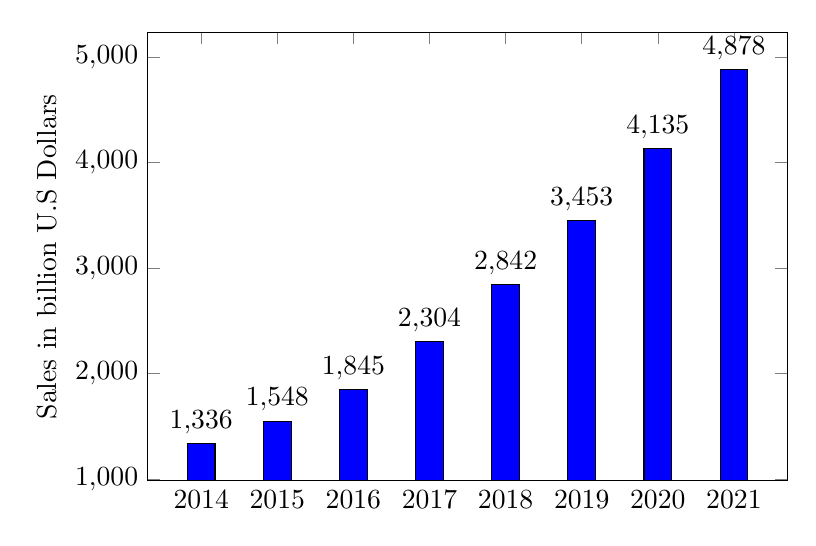
\begin{tikzpicture}
        \begin{axis}[
            symbolic x coords={2014, 2015, 2016, 2017, 2018, 2019, 2020, 2021},
            ylabel=Sales in billion U.S Dollars,
            width=0.8\textwidth,
            height=0.6\textwidth,
            nodes near coords,
            nodes near coords align={vertical},
          ]
            \addplot[ybar,fill=blue] coordinates {
                (2014,  1336)
                (2015,  1548)
                (2016,  1845)
                (2017,  2304)
                (2018,  2842)
                (2019,  3453)
                (2020,  4135)
                (2021,  4878)
            };
        \end{axis}
    \end{tikzpicture}
\caption{Worldwide e-commerce sales growth from 2014 to 2021}
\label{fig:ecommerceGrowth}
\end{figure}

This behavior is result of two facts. Firstly, society is more trustful on technology and the fear of fraud is more reduced now due to the current legislation, certifications given to trusted online stores and because new web-oriented payment methods having risen. The second reason is the high market competition that exists nowadays. Unlike the 90s and the early years of the \nth{21} century, there are a lot of online stores, selling almost everything that a customer might need.
\par

Despite the existence of ever more online stores and e-commerce platforms, the great majority of these platforms are engaged in the trade of physical products.

\section{E-Commerce applied to services}
\label{sec:ecommerceAppliedToServices}
As was explained on section \ref{sec:ecomIndustry}, most of e-commerce is done for buying physical products. This is done in the so called "online stores". However, the sale of services is a more contained, niche, market within this industry. Most of the services that are sold online are typically also virtual. Examples of those services are web hosting, cloud services and email accounts. It is, nevertheless, also possible to order some services online, like ordering an insurance contract but the range of options that exist is much more restricted.
\chapter{State of the Art} % Main chapter title
\label{chap:StateOfTheArt}
Developing a platform that supports multiple types of services and with the ability to grow in terms of both features and traffic, requires it to be built with the best quality standards of software engineering. In this chapter, we will firstly analyze approaches of other platforms already on the market, and present the state of the art on software architecture, by researching on several architectural designs that might be applicable to this project.

\section{Existing Solutions}
In this section will be presented some existing solutions that have similar requirements to this project. The analysis of these platforms will help to understand what problems may arise, and how these companies tackled them.

\subsection{UberEats}
With the success that Uber was having in the passenger transportation sector, in 2014, the company started on the food delivery business. Initially, this was a side project that was integrated Uber's main app. The service was only available for lunch, and number of options were scarce. Note that this occurred in a time where there were already other competitors offering food delivery services, without these restrictions \parencite{whyUberStartedUberEats}. 
\par
UberEats is a food delivery service offered by Uber, that connects several restaurants to the customers in the restaurant's surrounding area. Contrary to what the competition was doing, UberEats limited the access to place orders to customers in zones where there were restaurants in their network \parencite{whyUberStartedUberEats}. This decision allowed three things: first, to increase the quality. It is impossible to keep the quality of a product after it had to go through several kilometers in order to be delivered to the customer. Second, it diminished the delivery time. People want to be able to order food minutes before lunch/dinner time. By limiting the areas where it was available, it was also possible to increase speed time. Last, but not the least, it enabled to keep a low, flat rate for all delivery services.
\par
Uber, and by consequence UberEats, is a company that was, since the beginning, very mobile oriented. Mobile e-commerce has grown a lot in the last ten years. In fact, since 2017, it counts for over half of the whole web traffic \parencite{percentageMobileTraffic}. The rise of the smartphones and with telecommunication companies offering better and cheaper services was a key fact that enabled this rise in the mobile share. This behavior is even more noticeable when the data relative to e-commerce is analyzed. The graph in figure \ref{fig:mobileGrowth} refers to the growth of the market share for mobile e-commerce\footnote{data retrieved from https://hostingfacts.com/internet-facts-stats/}. In 2018, the market share for mobile e-commerce was 63.5\%, and it is expected to grow as high as 72.9\% until 2021.

\begin{figure}[ht]
\centering
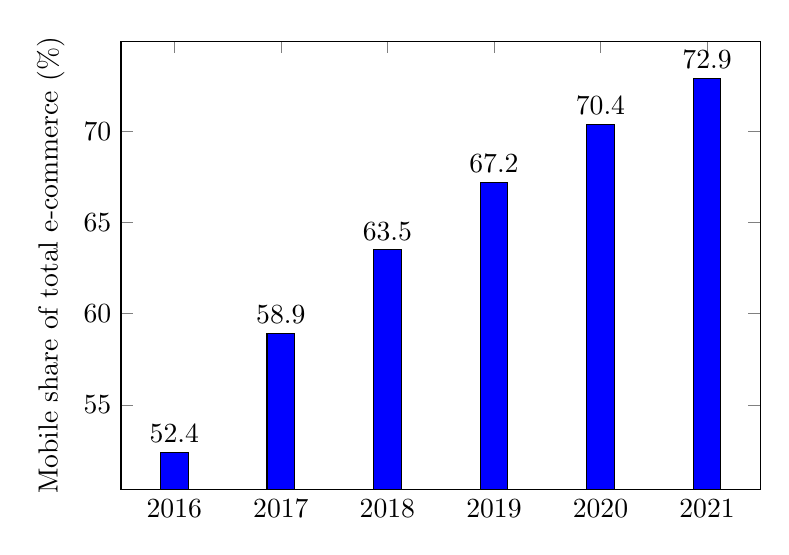
\begin{tikzpicture}
        \begin{axis}[
            symbolic x coords={2016, 2017, 2018, 2019, 2020, 2021},
            ylabel=Mobile share of total e-commerce (\%),
            width=0.8\textwidth,
            height=0.6\textwidth,
            nodes near coords,
            nodes near coords align={vertical},
          ]
            \addplot[ybar,fill=blue] coordinates {
                (2016,  52.4)
                (2017,  58.9)
                (2018,  63.5)
                (2019,  67.2)
                (2020,  70.4)
                (2021,  72.9)
            };
        \end{axis}
    \end{tikzpicture}
\caption{Mobile share of total e-commerce 2016 to 2021}
\label{fig:mobileGrowth}
\end{figure}

This means that Uber was right on the start of the mobile trend, when it started, which was a very positive factor when evaluating the growth of their business.

\subsection{Glovo}

Glovo started in 2015 with a business model similar to UberEats. However, the two companies differed on what products they delivered. While UberEats is focused on food delivery, Glovo has a broader range of products that they are able to deliver. According to Glovo's website, they are able to deliver "food, gifts, markets, pharmacy, snacks \& juices, anything". As the company advertises, in addition to the services that they provide (ordering food, medicine...), the platform is also able to process and deliver miscellaneous items, defined by the customer. 
\par
Despite the possibility for the customer to order almost anything on Glovo, the most used service is, actually the food delivery. This makes Glovo a competitor to Uber Eats which customers choose, typically, based on price and delivery time. Glovo also offers certain options that are not available in UberEats. An example of that is the possibility to add instructions of how well done the meat is wanted. On the other hand, UberEats provides an estimated delivery time, while Glovo only offers abstract information about the status (for example, "your Glovo is being collected") \parencite{uberVsGlovo}.
\par
Similarly, the approach was unsurprisingly very mobile driven, since when the company started, the mobile phenomenon was already very prominent. Nevertheless, taking into account the figure \ref{fig:mobileGrowth}, it was a good decision, since the mobile share on total e-commerce keeps growing.

\section{Technology}
\label{sec:StateOfTheArt_Technology}
In this section the current state of the art in terms of technology will be analyzed. Architecture and developing frameworks are the topics that will be discussed in the next pages. The research done for these topics is essential to fully understand the pros and cons of each approach, and how they fit (or not) this project.

\subsection{Architecture}
\label{sub:StateOfTheArt_Technology_Architecture}
As it is in the software development life cycle, the first topic that will be tackled is the architecture. This research will help the understanding of the best practices in terms of software design, and which approaches are a better fit for this project.
\par
Architecture can be defined as the structure of the various components within a system, how the communicate with each other, the constraints, principles and guidelines. It must be taken into account that these last three points are dynamic and often change over the time \parencite{mappingServicesToActivities}. In the next few sections, the architectural styles \gls{SOA}, Micro-Services, and \gls{CQRS} will be presented.

\subsubsection{Service Oriented Architecture}
\gls{SOA} is an architectural style that has as its main purposes, the focus on the business, modularity and reuse. It consists in splitting the system's functions into small applications, each one representing a real business activity. That business activity is what is called a service. The services that exist in a system must provide an interface in order to communicate with other services.
\par

The systems that follow this architecture may be called service-oriented applications. These applications typically follow an architecture similar to the one presented in figure \ref{fig:soaExample}. 
\par
\begin{figure}[ht]
\centering
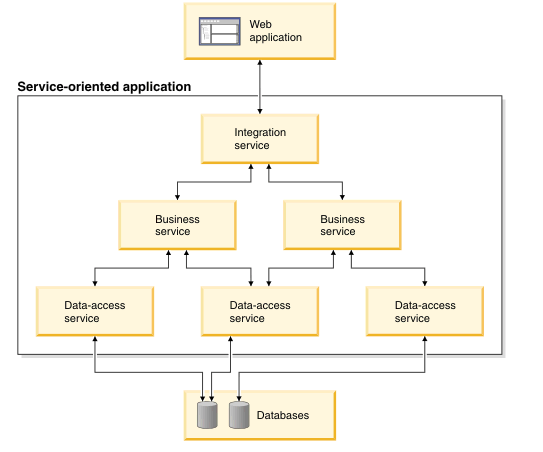
\includegraphics[width=0.8\textwidth,keepaspectratio]{chapters/State_of_the_Art/assets/soa_arch.png}
\caption[Service Oriented Architecture Example]{Service Oriented Architecture Example\footnotemark}
\label{fig:soaExample}
\end{figure}
\footnotetext{retrieved from \url{https://www.ibm.com/support/knowledgecenter/en/SSMQ79_9.5.1/com.ibm.egl.pg.doc/topics/pegl_serv_overview.html}}


\par
This architectural style is one of the most common on companies. In fact, "it has become the excellent methodology of system construction" \parencite{soaPetroleum}.
\par
The architecture is composed of three main blocks. The topmost level is where are the responsible for the integration of the application with external services/applications. This is often accomplished with an \gls{ESB}. An \gls{ESB} is communication system that abstracts the conversion of different protocols into a single component. This layer communicates with the business services. The business services are located in the second layer of the application and processes low-level business operations. The business logic inherent to the system, would be implemented in this layer. The integration layer will call several business services in order to process a business operation. Taking the e-commerce example, when processing an order, the business services could be fetching the information of the product, calculate order values and process invoice. Lastly, the third level of the architecture consists of data-access services, responsible to retrieve and persist information in the database. The business services use this layer in order to have access to the information and then return it, when processed, to the integration layer. It may also happen the other way around. For create/update operations, when the integration service passes information onto the business services, that information will be processed and sent to the data-access layer, where it will be persisted in the database. In addition to databases, it may also access message queues to send events \parencite{soaIBM}.


\par
\gls{SOA} has many variations and extensions, applying new patterns and good practices adapted to new realities. Micro-Services is one of them.

\subsubsection{Micro-Services Architecture}
\label{sub:StateOfTheArt_Architectures_microservices}
Micro-Services, or Micro-Services Architecture, are a part of \gls{SOA} where the services are more fine grained. These services should be independent of each other in order to be as loosely coupled as possible. Micro-Services Architecture is widely known for following the \gls{SRP}, since its function within the system is very well defined.
\par
This approach is perfect for complex systems, given that they are typically heterogeneous, unbounded and dynamic. The architecture of these systems must employ a high level of abstractions, to be able to deal with the complexity of these systems. 
\par
A service that consumes another, doesn't need to know any internal logic of it, as long as a clear interface has been defined. The interface is what is responsible for the establishment of a contract that enables a consumer to be able to communicate. Each of these services must be autonomous. This means that, as long as none of the contracts has been broken, each service is responsible for itself. For example, in a product service, that has as its main responsibility, the management of the products on an e-commerce platform. As far as the contracts established are not broken (no longer be able to create products in the same way, is a good example of this), the service may change the way it manages the products. This also means that consumers must be abstracted of how, in this case the product service, works internally and just use the contracts, as a service.
\par

\begin{figure}[ht]
\centering
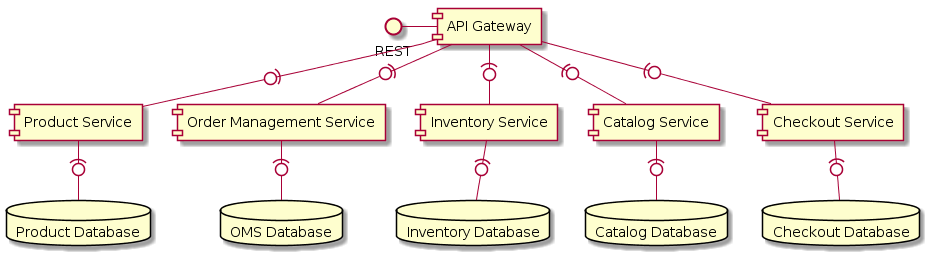
\includegraphics[width=\textwidth,keepaspectratio]{chapters/State_of_the_Art/assets/SOA_example.png}
\caption[Microservices Architecture Example]{Microservices Architecture Example}
\label{fig:microservicesExample}
\end{figure}

\par
In figure \ref{fig:microservicesExample} is presented an architectural example of micro-services. This example follows the one previously mentioned of an e-commerce platform. In the figure, it is possible to verify that the responsibilities are divided into five services:
\begin{itemize}
  \item \textbf{Product Service}, with the responsibility of managing the existing products on the platform;
  \item \textbf{Order Management Service}, which is responsible for processing the orders;
  \item \textbf{Inventory Service}, is who is responsible for managing the quantity of each product that is available;
  \item \textbf{Catalog Service}, managing which products are available and when;
  \item \textbf{Checkout Service}, with the responsibility of finishing the order on a front-office side and process the payment.
\end{itemize}

\par 
As it was mentioned, these services are completely loosely coupled since there are no dependencies between any of them. Every service is also entitled and responsible for maintaining its own database, where it will store the data necessary to its correct functioning. In a well implemented micro services architecture, it should also be possible to deploy each of the services independently, without impacting the correct functioning of the others.


\subsubsection{Command Query Responsibility Segregation}
\label{sub:StateOfTheArt_Architecture_CQRS}
\gls{CQRS} is a pattern described by Greg Young where it is defended that the models used to update information and the models used to read information can be different \parencite{cqrs}. The most common use of a database is often a \gls{CRUD} approach. This means that all create, read, update and delete operations use the same model. This approach often brings some disadvantages. It can turn the management of permissions and security into a more complex task, since each entity is target of both read and write operations. It may also lead to an information mismatch since some fields may not be required some information that is already existent in the database. Finally, it may create concurrency problems, when a set of services operate over a given amount of data. This might also create performance issues, since read and write operations can't be scaled independently \parencite{microsoftCqrs}.
\par

This separation maps directly with the command and query concept. Write operations, like \gls{CRUD}'s create, update and delete actions, are commands. Read operations that solely retrieve information are considered queries.
\par
This pattern separates these two operations by having two different interfaces. By doing this, the possibility of having different models is also enabled. On the other hand, \gls{CQRS} can't be automatically generated by scaffold mechanisms as \gls{CRUD} can \parencite{microsoftCqrs}. \gls{CQRS} is often implemented by having two different services, one responsible for the queries, other responsible for the commands. This allows to scale the system independently, which can be useful on services that have a high load of reads, but not many updates.

\par 

\gls{CQRS} is recommended to be used only in specific parts of a system. In particular, parts where there is a high chance of concurrence and/or parts where \gls{DDD} was used. It is also a good option for systems that need to handle high performance applications, because, not only as said earlier, it is possible to scale independently, but also because is possible to add different optimization to each side \parencite{cqrs}.
\par

In the figure \ref{fig:cqrsExample}  there is a schema of a typical \gls{CQRS} implementation. It is possible to see the two interfaces that are available, one for the queries, and other for the commands. In case of the command, the interface is connected to its model where it will validate the user/consumer's input and, then, proceed to the operation in the database. For the queries, the behaviour is very similar. After the user/consumer's request, it is sent to the model, which then retrieves the data from the database and processes it. Finally, the information is returned to the requester.

\par

\begin{figure}[t]
\centering
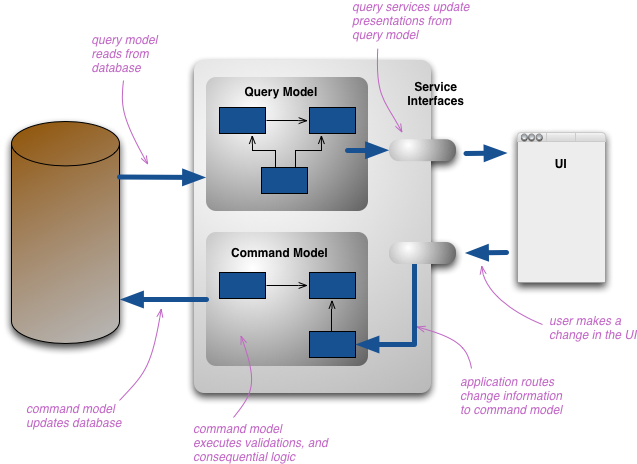
\includegraphics[width=0.8\textwidth,keepaspectratio]{chapters/State_of_the_Art/assets/cqrs.png}
\caption[CQRS Typical Implementation]{CQRS Typical Implementation\footnotemark}
\label{fig:cqrsExample}
\end{figure}
\footnotetext{retrieved from https://martinfowler.com/bliki/CQRS.html}
\par

\gls{CQRS} is a very powerful architecture that solves many specific problems. However, before deciding to use this pattern, a careful analysis should be carried out. The implementation of this pattern requires a change in mindset and many information systems fit in the traditional approach, and implementing \gls{CQRS} would add unnecessary complexity to the project \parencite{cqrs}.

\subsubsection{Event Sourcing}
\label{sub:StateOfTheArt_Architecture_EventSourcing}
Event sourcing is an architectural style, where every change in the state of an entity triggers an event, and that the event is stored in the same sequence that they were applied. The whole purpose of doing this is to replicate the state of a certain entity by reprocessing all the events \parencite{martinFowlerEventSourcing}.

\par
This architecture also passes the responsibility of calling all operations inherent to a business process to the services that actually do that operations. In contrary to \gls{HTTP} calls, where the source (which triggers the event) needs to know processes to call, in event sourcing (and most event-driven architectures), the source only needs to make sure that the event is published. The listeners are the ones who need to check if that particular event is something that needs to start any operation
\par
The figure \ref{fig:kafkaEvent} presents an example for this situation. The user sends a request to the front-end server, which then publishes an event to the Kafka Broker. When this happens, both "First Service" and "Second Service" will receive the information about what happened, and then decide if they should trigger any process regarding the user action.

\begin{figure}[ht]
\centering
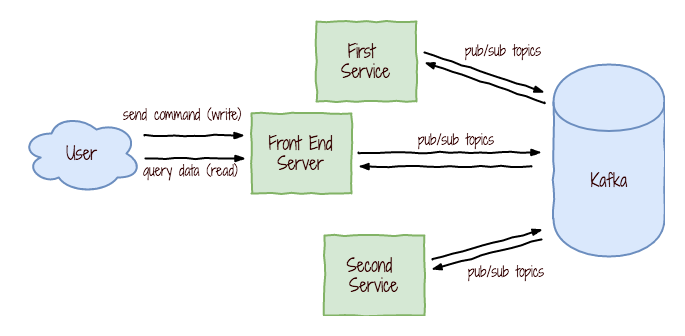
\includegraphics[width=0.8\textwidth,keepaspectratio]{chapters/State_of_the_Art/assets/kafka-event-sourcing.png}
\caption[Event Driven Architecture using Kafka]{Event Driven Architecture using Kafka\footnotemark}
\label{fig:kafkaEvent}
\end{figure}
\footnotetext{retrieved from \url{https://medium.com/kontenainc/event-sourcing-microservices-with-kafka-2568801527d8}}


\par

This architecture is very good for any application that needs to keep track of every change that occurred on a certain entity of their business. Bank systems are a good example where this architecture may be used. There must be a record of every transaction that is made in a bank account and with event sourcing, that is done, and the events produced will trigger the necessary processes to run. 

\subsection{Software Development Frameworks}

In this section, an overview will be given over the current most used software frameworks. These frameworks are used as abstractions over more specific \gls{OS} code, thus enabling its re-use. Furthermore, they provide several libraries, tools and compilers to facilitate the developer's work. Currently, the use of these abstractions is a standard to build and deploy applications within the industry. In the next sections, we will analyze the frameworks .NET Core, Java Spring and Node.js.

\subsubsection{.NET Core}
\label{sub:StateOfTheArt_Frameworks_NET}
.NET is a software framework, developed and maintained by Microsoft that was released in 2002. This framework provides a large class library, \gls{FCL}, that includes the main standard libraries, and language interoperability. This means that it is possible to use code written in other language of the .NET platform. This is possible because .NET runs in a software environment, rather than a hardware environment. This is a virtual machine called \gls{CLR}.
\par
This platform also provides tools to create applications for several types of devices (phones, tablets, etc.). These applications can be console apps, Windows Forms Apps or \glspl{API}. When it comes to web development, .NET has a web application framework specifically for that. ASP.NET was released within the .NET Framework and was the successor of \gls{ASP}, built on top of the \gls{CLR}.

\par
The possibility to use the \gls{CLR}, offers the possibility to develop applications in the ASP.NET platform using different languages, within the range available. Languages like C\#, Visual Basic and F\# are all supported and be called directly in the code. 
\par

One of the main problems of the .NET Framework, was that it was only prepared to run on Windows Environments. These servers are often more expensive and slower than the Linux Servers. Java Spring, one of .NET's biggest competitors, doesn't have this restriction and can run on any environment and \gls{OS}. To fight this problem, in 2016, Microsoft launched .NET Core 1.0 as an alternative to the traditional .NET Framework. Since then, the maintainers have kept on developing the platform. The version 3.0 was announced on Microsoft Build on May 2018 and it is expected to be released in 2019 \parencite{whatIsDotNet}.

\par
The development environment for any .NET project is the Visual Studio. This \gls{IDE} has lots of useful tools for development, including the integration with Azure, allowing direct deploys via Visual Studio. As the graphic of figure \ref{fig:topIdes} presents, Visual Studio is the second most used development environment only bellow Visual Studio Code, which is also developed by Microsoft.
\par

\begin{figure}[ht]
\centering
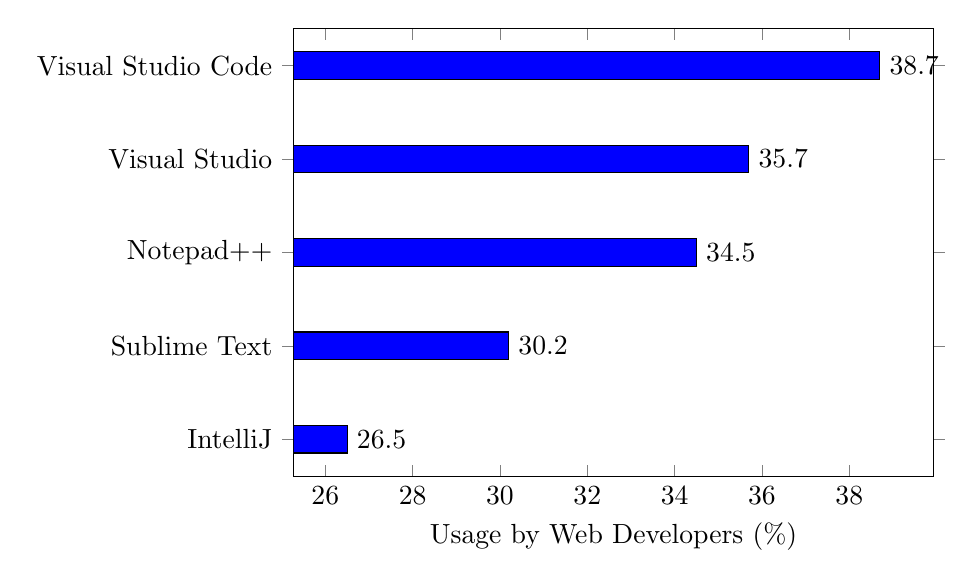
\begin{tikzpicture}
        \begin{axis}[
            symbolic y coords={IntelliJ,Sublime Text,Notepad++, Visual Studio,Visual Studio Code},
            xlabel=Usage by Web Developers (\%),
            width=0.8\textwidth,
            height=0.6\textwidth,
            xbar,
            nodes near coords,
            nodes near coords align={horizontal},
          ]
            \addplot[xbar,fill=blue] coordinates {
                (26.5,IntelliJ)
                (30.2,Sublime Text)
                (34.5,Notepad++)
                (35.7,Visual Studio)
                (38.7,Visual Studio Code)
            };
        \end{axis}
    \end{tikzpicture}
\caption[Top 5 most used IDEs by Web developers]{Top 5 most used IDEs by Web developers \footnotemark}
\label{fig:topIdes}
\end{figure}
\footnotetext{data retrieved  from https://insights.stackoverflow.com/survey/2018/}
\par


ASP.NET also offers automatic monitoring built in. This allows the maintainers to monitor the applications for some basic problems (like infinite loops or memory leaks) and immediately take action to solve the problem. This ensures the higher stability of the application \parencite{prosAndConsNetCore}.

\par


However, the support of data-oriented development for .NET (and not just .NET Core) is provided by Entity Framework. Entity Framework is an \gls{ORM} that connects the model of the application to relational databases. This framework is thought to offer low flexibility and not support all database designs. The fact of the development environment being Visual Studio also brings problems. The licensing costs of the \gls{IDE} is about \$45 per month/user for the base version\footnote{prices retrieved from https://visualstudio.microsoft.com/pt-br/vs/pricing/ on 16/02/2019}. Some people also complaint about the technology being too connected to its vendor, Microsoft \parencite{prosAndConsNetCore}. As opposed to other frameworks that are much more community-driven, .NET still depends on decisions made by Microsoft, which may lead to offer no alternatives for integration that the ones that are distributed by them.


\subsubsection{Java Spring}
\label{sub:StateOfTheArt_Frameworks_java}
Java Spring is an open-source application framework that provides core features to the Java platform. The first version of this framework was released in 2002 by Rod Johnson as a beta, reaching to a stable version in 2004. Despite being an open-source platform, it is maintained by Pivotal.

\par

Java Spring is a very flexible framework that supports both \gls{XML} and annotations for configuring the Spring Beans. The beans are the backbone of the application that are instantiated, assembled and managed by the Spring \gls{IoC}. The \gls{IoC} is "a process in which an object defines its dependencies without creating them" \parencite{whatIsASpringBean}

\par
This framework provides support for several services, like \gls{AOP} for cross-cutting concerns, Authentication and Authorization, dependency injection and testing infrastructure, to write unit and integration tests. There is also a data access framework that abstracts the developer from many common difficulties that are faced. The most common data access frameworks for Java, such as \gls{JPA} and Hibernate are also supported \parencite{springFramework}. 
\par

Spring also offers support for \gls{JDK} timers, logging frameworks and libraries that contain many useful functions for the developers to learn and use them to develop applications \parencite{prosAndConsJavaSpring}. 

\par
Being built on top of Java, this means that it will run on the \gls{JVM}. The \gls{JVM} is a virtual machine that runs on top of the \gls{OS}, abstracting its procedure calls and standardizing them for the programming language. This means that an application that was built using Java Spring, can run on any \gls{OS} \parencite{whatIsTheJVM}. This was a great advantage that Java had over its competitors, specially on the web development industry. Competitors like Microsoft's .NET didn't support cross-platform. However, in 2016, Microsoft presented .NET Core. A framework based on .NET but that could run on any machine. 
\par 
Two of the main cons of the Spring Framework are its complexity and the long learning curve. This happens due to the 2400+ classes plus tools that the developers need to know to be able to develop their applications \parencite{javaSpringAdvantagesAndDisadvantages}. This can make the project far more complex than what it needed to be. Also, there are no clear security guidelines. Cross-site scripting attacks or cross-site request forgery attacks avoidance are examples of documentation that is missing \parencite{prosAndConsJavaSpring}.

\subsubsection{Node.js}
\label{sub:StateOfTheArt_Frameworks_Node}
Node.js is a \gls{JS} runtime environment. It uses the Google Chrome V8 engine in order to run the code. As JavaScript was originally made to run in the client application, Node was born to extend the language to the back-end side \parencite{whatIsNodejs}.
\par
Node's main idea was to "use non-blocking, event-driven I/O to remain lightweight and efficient in the face of data-intensive real-time applications that run across distributed devices" \parencite{whyUseNode}. That means that this technology didn't come to overcome every problem ever faced. Instead, it solves a particular need in the development world. For example, as Node is single threaded, it is not indicated for heavy \gls{CPU} operations. The main advantage or using it is to build fast, scalable and lightweight applications. Another benefit of using Node.js is that both the front-end and back-end will be in a common language. This causes for a fast synchronization, which is especially good for event-based applications \parencite{goodAndBadOfNode}. 
\par
The way how it works is different from the traditional implementations. On that approaches, each new request would start a new thread in the system, using its \gls{RAM}. When the available memory is all in use, the new connections will stay on-hold, waiting for a thread to be available. On the other hand, Node.js uses non-blocking I/O calls, which allows it to handle "tens of thousands of concurrent connections" \parencite{whyUseNode}. The figure \ref{fig:nodeThreadManagement} demonstrates the difference between the thread management done in both the traditional applications and in Node.js.
\par


\begin{figure}[ht]
\centering
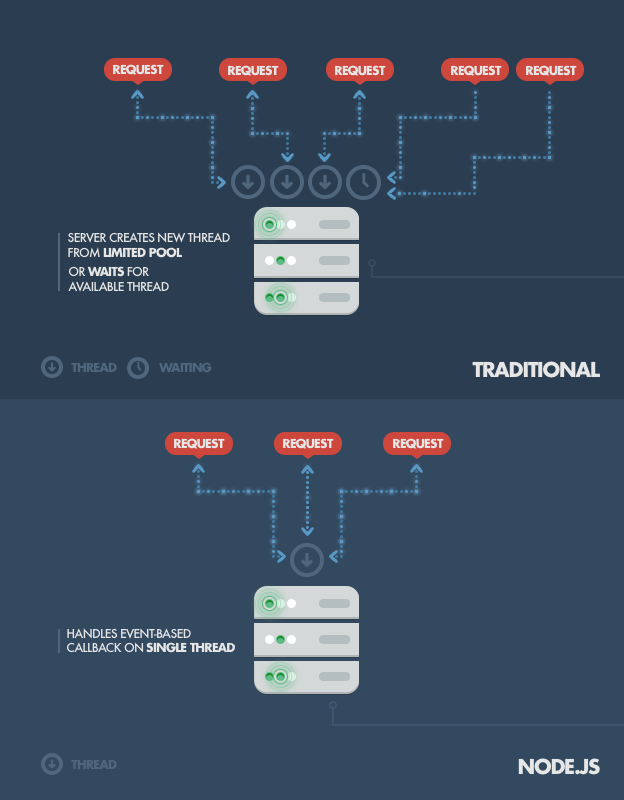
\includegraphics[width=0.8\textwidth,keepaspectratio]{chapters/State_of_the_Art/assets/node-functioning.png}
\caption[Node.js Thread management]{Node.js Thread management\footnotemark}
\label{fig:nodeThreadManagement}
\end{figure}


\par
All the points that were referred above, make Node.js as a perfect platform to be used in applications such as chat rooms, data streaming systems and stock trading platforms.
\par

As every good thing has a but, Node is no exception. Despite being a quite new technology, the core of node modules is considered stable. However, many tool on npm (the Node.js package manager) are of poor quality and/or have not being properly documented \parencite{goodAndBadOfNode}. The fact of being open-source also has an impact. Despite the core modules being supervised by Joyent and other major contributors, the rest of the tools might lack in the code quality. There are also some performance problems when working with Node. As JavaScript was made to be asynchronous, it has a non-blocking \gls{I/O} model. This means that it can process many reads and writes that are queued in the background, without blocking the main thread. For this, Node uses callbacks. Callbacks are functions that run on background in a queue. If there is a situation where callbacks are nested within other callbacks, it will make the code difficult to read a maintain. This is commonly known as callback hell. The listing \ref{lst:callback_hell} presents an example of this problem.
\footnotetext{retrieved from https://www.toptal.com/nodejs/why-the-hell-would-i-use-node-js}
\par

\begin{minipage}{\linewidth}
\lstinputlisting [caption={Callback Hell example\protect\footnotemark.},
label=lst:callback_hell]
{chapters/State_of_the_Art/assets/callback-hell.js}
\end{minipage}
\footnotetext{retrieved from http://callbackhell.com/ on 16/02/2019}

\par
 Node is constantly chosen for solutions that require real-time updated data, like video-conference systems or online gaming. By using \gls{JS} programming language, the learning curve for Node is kept to a minimum. This means that developers with front-end experience (which requires a lot of JavaScript) can start programming server-side without facing many difficulties. The fact of being a lightweight makes this a very good option for micro-service architectures. Despite being an open-source technology, it has a great corporate support. That support was initially provided by Joyent, but in 2015, with the creation of the Node.js Foundation, IBM, Microsoft, Paypal, SAP and Fidelity also offered their support by becoming founding members or the organization \parencite{goodAndBadOfNode}.
\par


\subsection{Swagger}
\label{sub:swagger}
Swagger is an open-source framework that allows the generation of automatic documentation of the available endpoints in an \gls{API}. This is done without any human intervention. Swagger is capable to ask the \gls{API} for an YAML or a JSON file that contains a detailed structure of the entire \gls{API}. This file is essentially a resource listing using the OpenAPI specification. This file contains the following information \parencite{whatIsSwagger}:
\begin{itemize}
    \item What are the operations supported by the \gls{API};
    \item What are the endpoint's parameters and return values;
    \item Authentication and Authorization information.
\end{itemize}

\begin{figure}[ht]
\centering
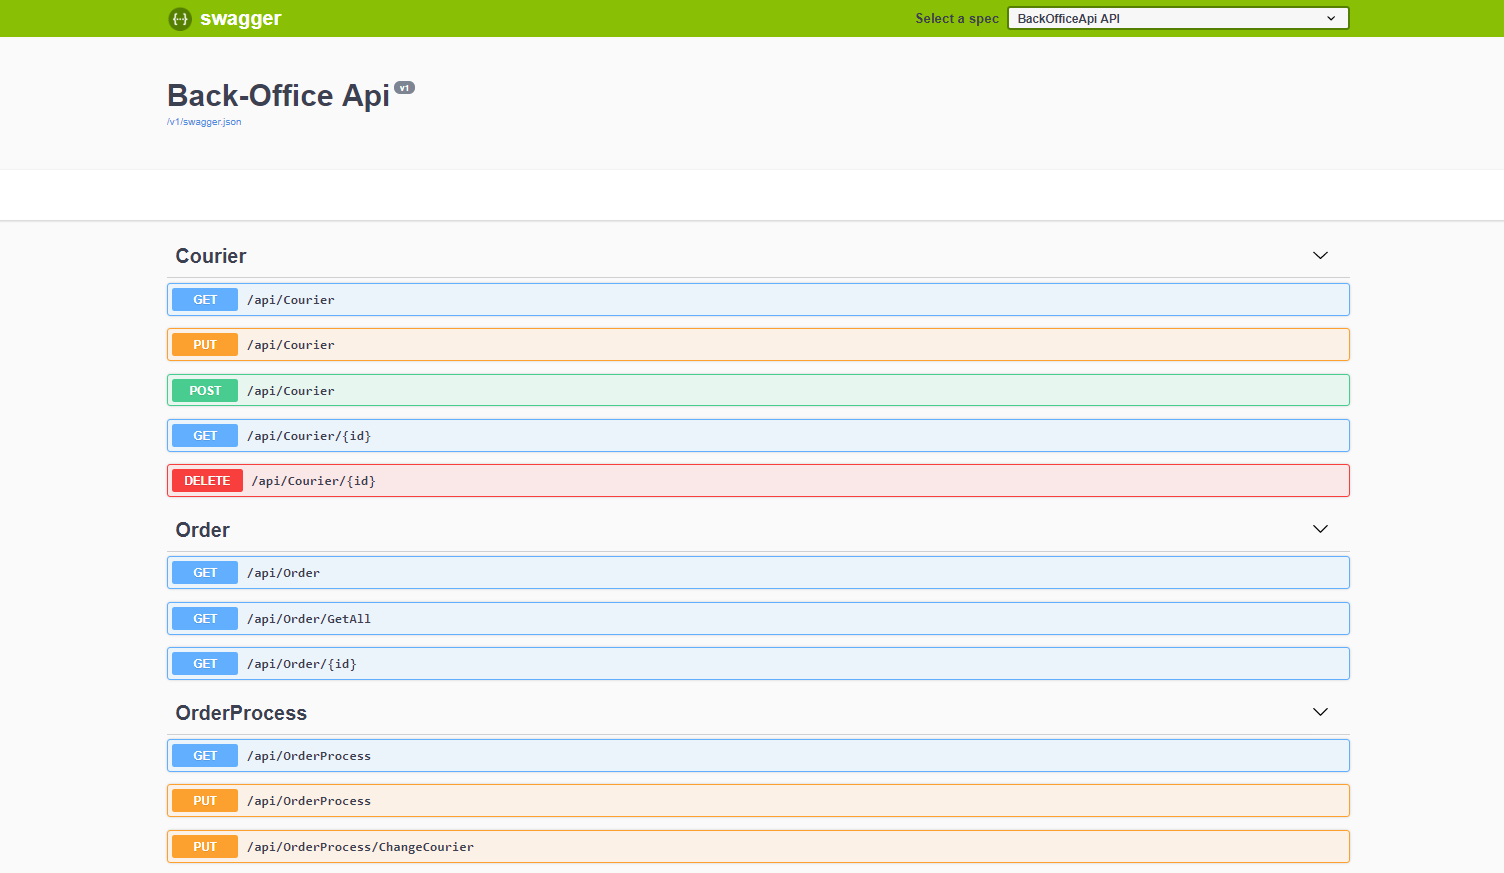
\includegraphics[width=\textwidth,keepaspectratio]{chapters/State_of_the_Art/assets/backoffice-api-endpoints.PNG}
\caption[Back-Office API Endpoints on Swagger page]{Back-Office API Endpoints on Swagger page}
\label{fig:swaggerEndpoints}
\end{figure}

\par
The figure \ref{fig:swaggerEndpoints} shows the listing of endpoints in one of the solution's \glspl{API}, Back-Office API. This allows the consumers to know from the start how to use the \gls{API}. Opening one endpoint, as shown in figure \ref{fig:endpointExample}, it is possible to verify the required parameters, the return value and even to call that endpoint, making it easier to make a direct request to the \gls{API}.

\begin{figure}[!hb]
\centering
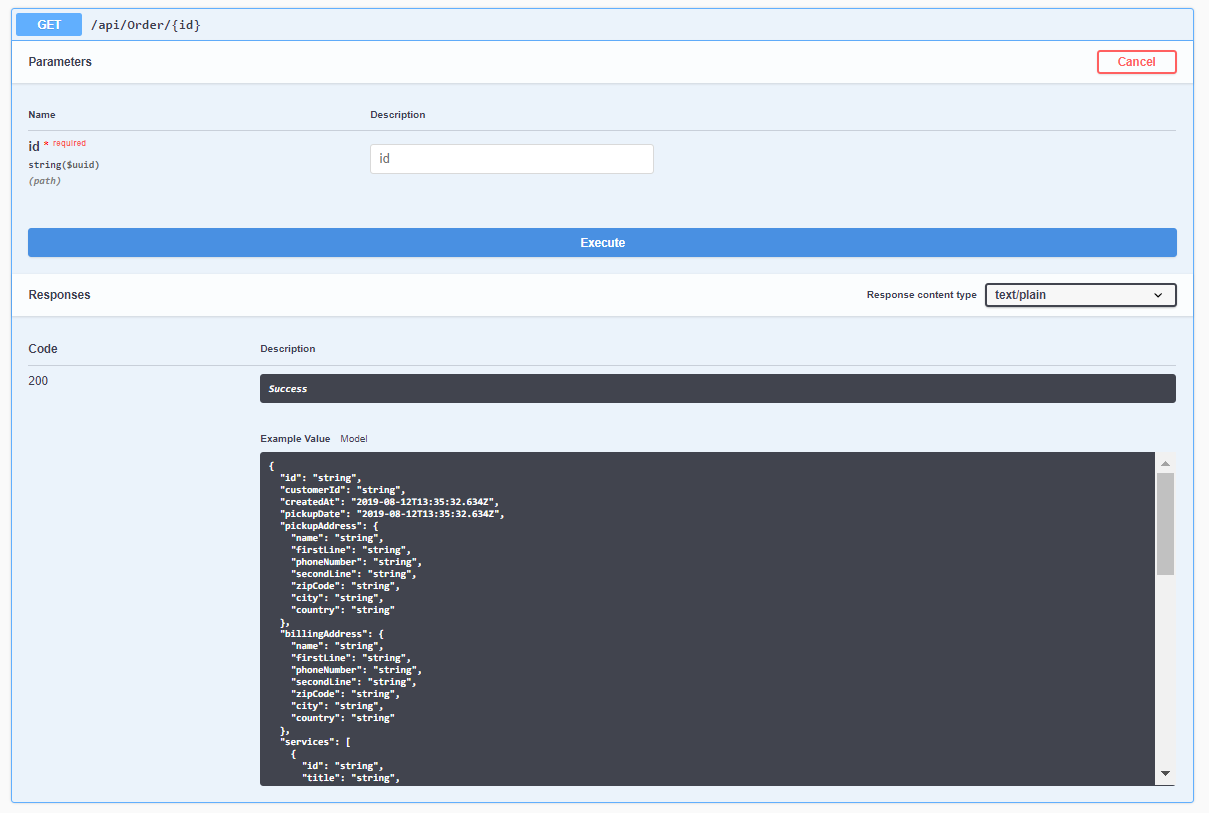
\includegraphics[width=\textwidth,keepaspectratio]{chapters/State_of_the_Art/assets/open-endpoint.PNG}
\caption[Open endpoint on Swagger]{Open endpoint on Swagger}
\label{fig:endpointExample}
\end{figure}

\par

Swagger has support for many languages and frameworks, such as .NET, Java, Go, C++, etc.

\chapter{Value Analysis} % Main chapter title
\label{chap:valueAnalysis}

Value is the most important concern when it comes to the development of an innovation and/or project. Not only in terms of monetary value, or cost, but specially the value that the product brings to the consumer. 
\par 
According to Lawrence D. Miles, the value of a product or service is attained when measuring the products performance and cost, where the product's performance is its ability to satisfy a certain need \parencite{valueAnalysisAndEngineering}. This means that the value of a product increases when it attains the highest performance at the lowest cost. In mathematics, value can be defined by the following formula:
\par
$$value= \frac{(Performance_x + Capability_x)}{Cost_x}$$
\par

This chapter provides an overview of the value analysis theory that will allow to understand fundamental concepts of this area of research. These concepts are essential to comprehend the value proposition that will also be presented in this chapter.

\section{New Concept Development}
Innovation is not a standard process. It requires a great ability of creativity, opportunity identification and problem solving. The \gls{FFE} is the first stage in that process. This is the point where, in most cases, the opportunities are found and ideas for a solution appears. This stage is a very experimental, unpredictable and unstructured one. As it requires a great amount of creativity, there is no standard process that will lead to a certain result. The results of this will influence the second stage of the process, the \gls{NPD}. This is the process of development and production of a solution to the opportunity that was found. Finally, the product would enter the commercialization phase, where it would be sold to the customers and start generating revenue. However, it was difficult to compare \gls{FFE} practices across different companies. This happens because there is a lack of common terms and definitions for this method's key elements. Without it, it is almost impossible to create new knowledge, or when it was possible, it would be ineffective \parencite{fuzzyFrontEndMethodsToolsThecniques}.
\par
To fill this gap and provide a common language on the front-end activities, Peter Koen and a group of researchers, developed a new theoretical construct, the \gls{NCD} model \parencite{commonLanguageForFFE}. In order to avoid the term \gls{FFE}, as it implies that the activity is mysterious, uncontrollable and unmanageable, Peter Koen introduced a new name for this stage, calling it \gls{FEI} \parencite{managingFrontEndInnovation}. The model is shown in figure \ref{fig:ncdModel}.
\par

\begin{figure}[bh]
\centering
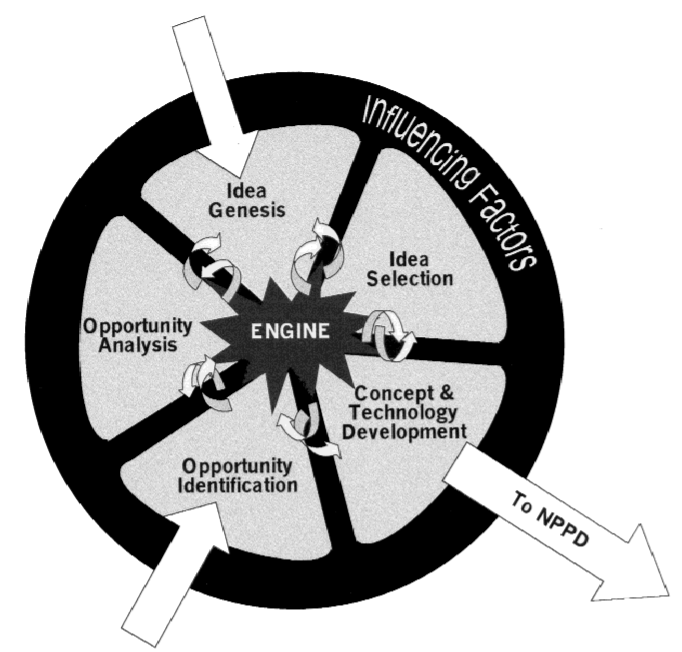
\includegraphics[width=0.8\textwidth,keepaspectratio]{chapters/Value_Analysis/assets/NCD_Model.png}
\caption[NCD model]{NCD model\footnotemark}
\label{fig:ncdModel}
\end{figure}
\footnotetext{retrieved from \url{https://web.stevens.edu/cce/NEW/PDFs/Clarity_FEE.pdf}}

\par
This model is composed by three distinct areas: the engine, at the center, the wheel, which are the five slices near the engine, and the rim, at the border of the model. The engine provides power to the innovation process. It is "fueled by the leadership and culture of the organization" \parencite{commonLanguageForFFE}. The wheel, is composed by five key activity elements: Opportunity Identification, Opportunity Analysis, Idea Generation and Enrichment, Idea Selection and Concept \& Technology Development. The third element, at the border of the model, consists on the external environmental factors that influence the engine and the activity elements. Examples of these factors may be the Business Strategy, Organizational Capabilities, the existent technology to be used and anything that is external to the organization (customers, competitors, trends, etc.). The arrows between the elements are there for the same reason why the model has a circular shape. To indicate that ideas flow and iterate between the five elements. The arrows pointing into the model represent the starting points that a project can have. It may start on either Opportunity Identification, or Idea Genesis. Projects will leave the \gls{FEI} by entering the \gls{NPPD} \parencite{commonLanguageForFFE}.

\subsection{Opportunity Identification and Analysis}
These elements refer, respectively, to the phases where a given company or individual identify an opportunity and analyze it to have a better perception of it and more information regarding the problem. The Opportunity Identification is the most common activity to serve as a starting point for a project, since it reflects a need that is yet to be fulfilled.
\par
It was the case of the project of this dissertation.  As it was already explained in sections \ref{sec:chap1_problem_statement} and \ref{sec:ecommerceAppliedToServices}, despite the existence of multiple online stores selling numerous products, when it comes to services, the number of options decreases drastically, and service providers, are already trying to offer a solution, without technology support. This creates an opportunity to innovate in this sector. Besides that, the existence of a pilot \gls{SP} available to work on the project also took a great part in the opportunity analysis.

\subsection{Idea Genesis and Selection}
The Idea Genesis is the first form of a solution to fulfill the needs found in the Opportunity Identification stage. It includes the process of birth, development and maturation of the opportunity into an concrete idea \parencite{commonLanguageForFFE}. To do this, companies often engage with customers and other companies and institutions in order to understand the real needs of their possible users, and link with cross-functional teams for brainstorming sessions, in order to have a more clear and open view of the whole picture. This element is also a common entry-point for projects. 
\par
In most cases, there are many possible solutions to a certain need. The vastness of good ideas also creates a new problem, which is to choose which ideas the company should select to proceed to the development stage \parencite{commonLanguageForFFE}. This turns out to be a very difficult task, since at this point there is a high degree of uncertainty and the information is very limited. Also, the \gls{ROI} is still a very foggy and risky guess.
\par
In the project in analysis in this thesis, there was already an idea for a solution. The first idea would be to create a solution to suppress the needs of the single pilot client that was already on-board, by developing a website where a customer could order laundry jobs and the \gls{SP} could manage its orders, connecting it to a network of couriers. However, in the first meetings with the student, a new idea surged. The idea was to create a platform, instead of a simple website for just one partner. By being abstracted to the \gls{SP} and the service that was being provided, the platform could easily scale. As the ideas matured, and using the decision process referred in the next sub section, it was decided to proceed with the last one, but taking into account that first partner would be a laundry, and focusing on those needs for the \gls{MVP}.

\subsubsection{Idea Selection using the Analytic Hierarchy Process}
The \gls{AHP}, is a multi-criteria decision method that uses mathematical techniques to aid in the decision makers to choose an option in a group of various alternatives. This process is based in the crossing of the alternatives with the existent criteria \parencite{whatIsAHP}.
\par
In order to select which of the ideas identified in the idea genesis phase, the \gls{AHP} was the method that was used for this. Firstly, an hierarchy decision tree was built:

\begin{figure}[htb]
\centering
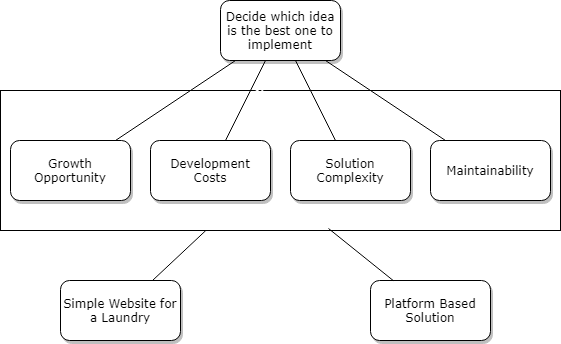
\includegraphics[width=\textwidth,keepaspectratio]{chapters/Value_Analysis/assets/Decision_tree.png}
\caption[Hierarchy Decision Tree]{Hierarchy Decision Tree}
\label{fig:decisionTree}
\end{figure}
\par

The figure \ref{fig:decisionTree} presents the hierarchy decision tree for the idea selection. The first layer reflects the main objectives of this analysis, which is to decide which of the ideas identified in the idea genesis, should be selected. On the second layer, the criteria that will be used for this analysis are presented. These criteria are:
\begin{itemize}
    \item \textbf{Growth Opportunity} - The possibility of the project reaching an higher level and gaining more partners;
    \item \textbf{Development Costs} - The costs in both time and money to develop a given solution;
    \item \textbf{Solution Complexity} - This measures the complexity of a solution for the user. In other words, if it will be difficult to use or not;
    \item \textbf{Maintainability} - This measures how easy, or not, the solution will be to add, remove or correct functionalities to the project.
\end{itemize}
\par

By having these criteria into account, it is possible to evaluate which decision is the best one to accomplish the main objective. The table \ref{tab:ahpEvaluation}


\begin{table}[ht]
\caption{AHP Evaluation Table}
\label{tab:ahpEvaluation}
\resizebox{\textwidth}{!}{%
\begin{tabular}{lllll}
 \textit{Criteria}                  & \textbf{Growth Potential} & \textbf{Development Costs} & \textbf{Solution Complexity} & \textbf{Maintainability}         \\ \cline{2-5} 
\multicolumn{1}{l|}{\textbf{Growth Potential}}    & \multicolumn{1}{l|}{1}    & \multicolumn{1}{l|}{5}     & \multicolumn{1}{l|}{4}       & \multicolumn{1}{l|}{2}           \\ \cline{2-5} 
\multicolumn{1}{l|}{\textbf{Development Costs}}   & \multicolumn{1}{l|}{1/5}  & \multicolumn{1}{l|}{1}     & \multicolumn{1}{l|}{3}       & \multicolumn{1}{l|}{1/2}         \\ \cline{2-5} 
\multicolumn{1}{l|}{\textbf{Solution Complexity}} & \multicolumn{1}{l|}{1/4}  & \multicolumn{1}{l|}{1/3}   & \multicolumn{1}{l|}{1}       & \multicolumn{1}{l|}{12/30}       \\ \cline{2-5} 
\multicolumn{1}{l|}{\textbf{Maintainability}}     & \multicolumn{1}{l|}{1/2}  & \multicolumn{1}{l|}{2}     & \multicolumn{1}{l|}{6}       & \multicolumn{1}{l|}{1}           \\ \cline{2-5} 
\multicolumn{1}{l|}{\textbf{Total}}               & \multicolumn{1}{l|}{2}    & \multicolumn{1}{l|}{8 1/3} & \multicolumn{1}{l|}{14}      & \multicolumn{1}{l|}{3,666666667} \\ \cline{2-5} 
\end{tabular}%
}
\end{table}

The growth opportunity and maintainability are the most important criteria in the decision, since they affect both what the solution can become in the future. The development costs and complexity are, nonetheless, factors to take into account since they can affect the delivery date. However, these last two are not as important as the first ones. 
\par

This matrix presents the normalized matrix in the \gls{AHP} evaluation method.

$M =
\begin{bmatrix}
0,5128 & 0,6000 & 0,2857 & 0,5455 \\
0,1026 & 0,1200 & 0,2143 & 0,1364 \\
0,1282 & 0,0400 & 0,0714 & 0,0455 \\
0,2564 & 0,2400 & 0,4286 & 0,2727 \\
\end{bmatrix}$

\par

Lastly, the table \ref{tab:ahpWeights} presents the weights of each criteria that was used for this decision.
\begin{table}[ht]
\centering
\caption[Weights of each criteria]{Weights of each criteria}
\label{tab:ahpWeights}
\begin{tabular}{ll}
\hline
\multicolumn{1}{|l|}{\textbf{Criteria}} & \multicolumn{1}{l|}{\textbf{Weight}} \\ \hline
Growth Potential                                                & 0,4860                                         \\
Development Costs                                               & 0,1433                                         \\
Solution Complexity                                             & 0,0713                                         \\
Maintainability                                                 & 0,2994                                        
\end{tabular}
\end{table}

\par
Hereupon, taking into account that the growth potential is the most important factor in this decision, the idea of developing a platform instead of a single website directed for a single laundry, was selected to fulfill the needs of this project, since a platform that supports multiple service providers, with different types of services is more likely to grow than a simple website for a laundry.

\subsection{Concept \& Technology Development}
The last element of the \gls{NCD} model is one of the most important. It serves as an exit door to development processes such as the \gls{NPPD}. This activity consists in the "development of a
business case based on estimates of market potential,
customer needs, investment requirements, competitor
assessments, technology unknowns, and overall project
risk" \parencite{commonLanguageForFFE}.
\par
For this project, this phase consisted in the development of the thesis formalization. This document states the problem and objectives of the project, mentioning also several requirements, constraints and restrictions.

\section{Value Proposition}
\label{sec:ValueProposition}
Value Proposition is one of the most widely terms used by companies, nowadays. However, it is difficult to find a clear definition for what it really means. Companies have been defining their \gls{CVP} in many different styles, with their perception of the concept \parencite{valuePropositionBusinessMarkets}. According to this same study, These definitions lie on three major types: all benefits, points of difference and resonating focus.
\begin{itemize}
    \item \textbf{All Benefits}: The most used by managers when asked to build a value proposition. This type simply consists in listing all the benefits that it is believed that the product/solution in question might provide. The more are listed, the better. However, this might lead the customer, to select which product to acquire just based on the price.
    \item \textbf{Points of Difference}: The second approach has the premise that the customer has alternatives other than the product that a given company is offering. As opposed to the previous type, points of difference focuses on the advantage of a product over its competition. It is focused on the question "why should a customer go with our product over our competitors'?" instead of "Why should I buy your product?". From a customer's point of view, this facilitates the process of choosing which is the best solution to his problem.
    \item \textbf{Resonating Focus}: Despite the advantages of the last point over all benefits, there is still room for improvement. The last approach focuses on two points that complement the previous type. This proposition "steadfastly concentrates on the one or two points of difference that deliver, and whose improvement will continue to deliver, the greatest value to target customers" \parencite{valuePropositionBusinessMarkets}. This means that instead of listing all the attributes and benefits of the product, and what differs the product over the competition, resonating focus defends that only the key aspects for the target customers should be mentioned. Secondly, this approach may contain a \gls{PoP}. A \gls{PoP} is a mandatory element for a customer to even consider the company's product as a viable option.
\end{itemize}
\par
Given the possible approaches for the value proposition, for the context of this thesis, it was chosen to follow the last approach, resonating focus. Since for this project, there will be three types of customers, it will be defined, also, three value propositions.

\subsection{Value Proposition for Final Customers}
The final customers are this project's most valuable stakeholder. If the platform doesn't meet the customers' needs, they will not use it, which means that there is no point for service providers to be present in the platform. Eventually, this could lead to the project not being viable.
\par
The value proposition for customers is as it follows:
\par
\begin{itemize}
    \item Choose from a range of service providers;
    \item On-click service request;
    \item Have any goods needed picked-up/delivered at your address, at your time;
    \item Pay with your phone. No need for counting change.
\end{itemize}
\par
Hereupon, the slogan that will be used to attract and present the value proposition to final customers will be:
\par
\textit{Focus on what is important. We take care of the boring tasks.}

\subsection{Value Proposition for Service Providers}
The service providers are the reason why the customers use the platform. Without service providers, there wouldn't be any customers and, by consequence, no business. The value proposition for the service providers is as it follows:
\par
\begin{itemize}
    \item Get online on a ready to use Platform;
    \item Be able to deliver and pickup at customer's address;
    \item Pay what you gain. You only pay fees over the services;
    \item Reduced costs when compared to a proprietary solution;
    \item Increase your range of customers.
\end{itemize}
\par
The slogan that will be used to attract and present the value proposition to service providers will be:
\par
\textit{Do what you do best. The logistics are on us.}

\subsection{Value Proposition for Couriers}
The couriers are the ones with the responsibility of carrying the goods from the customer to the \gls{SP} and vice-versa. It is a very important job since they are the only party to have direct contact to the final customer. The value proposition for couriers is as it follows:
\par
\begin{itemize}
    \item Flexible work hours;
    \item Be your own boss;
    \item Easy to get on-board;
    \item No usage costs;
    \item Increase your income.
\end{itemize}
\par
With this, the slogan that will be used to attract and present the value proposition to couriers will be:
\par
\textit{Create your own schedule and increase your income}

\section{Value for the Customer}
When developing a new product or service, one of the most important things that companies must have in mind, is the value that it will bring to their customers. However, this exercise is a harder task than it appears. The reason for this is because value is a subjective concept. It is a trade-off between benefits and sacrifices. Those benefits and sacrifices might have a different impact on distinct customer segments. What might be one's benefit, might be indifferent for other. Even if we look to the individual customer in a single segment, this phenomenon may occur due to the individuality of each customer. Nevertheless, it is expected to occur less often. Value may also be relative to the current competition on the market. When a certain company launches a product that has similar functions to a competitor's early released product, the customers are already used to that features, which makes it lose the novelty factor \parencite{relationshipValueAndRelationshipQuality}.
\par
\gls{VC} is described by Tony Woodall as 
\say{any demand-side, personal perception of advantage arising out of a customer’s association with an organization’s offering, and can occur as reduction in sacrifice; presence of benefit (perceived as either attributes or outcomes); the resultant of any weighed combination of sacrifice and benefit (determined and expressed either rationally or intuitively); or an aggregation, over time, of any or all of these} \parencite{conceptualisingValueForTheCustomer}. On this same study, Woodall divides \gls{VC} into two sub-forms: Nature of Derived \gls{VC} and Contingent \gls{VC}. The first one refers to \gls{VC} in its derived form. It focuses on excellence and more in derivatives as material value, functional value and emotional value. It is also called "Consumption Value" \parencite{weAreWhatWeBuy}. Most of these are types of value don't change over the time. The second one, focuses on the value on a longitudinal timeline, from the period before the customer buys the product, passing for the transaction it-self and ending in the after use. The whole process is part of the experience in Contingent \gls{VC}. 
\par

\begin{figure}[htb]
\centering
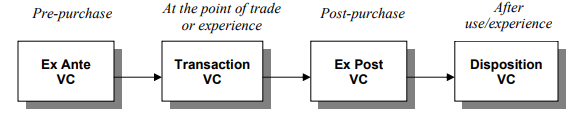
\includegraphics[width=\textwidth,keepaspectratio]{chapters/Value_Analysis/assets/contigent-value-phases.png}
\caption[Longitudinal Perspective on \gls{VC}]{A Longitudinal Perspective on \gls{VC}\footnotemark}
\label{fig:longitudinalVC}
\end{figure}
\footnotetext{retrieved from \url{https://cdn.ymaws.com/www.ams-web.org/resource/resmgr/original_amsr/woodall12-2003.pdf}}

\par
In the figure \ref{fig:longitudinalVC}, it is possible to verify each of the temporal phases inherent to the Contingent \gls{VC}. Each of these temporal stages have associated values, benefits and sacrifices. 
\par
The table \ref{tab:contingentVCMapping} presents a mapping between each of the temporal phases of the Contingent \gls{VC}, and some of its associated values, benefits and sacrifices, for the project in analysis in this thesis. As was already exposed in exposed in section \ref{sec:ValueProposition}, there are three different clients of this system: the final customer, the service provider, and the courier. Since the main problem to be solved by this project will be a problem of the service providers, the mapping was done for the benefits and sacrifices of that specific client. 
\par
Focusing on the benefits and the sacrifices, it is verified that there are many benefits for the customer and just a few sacrifices, most of them related to the price and training costs.
\par
\begin{table}[ht]
\centering
\caption{Contingent VC Temporal Stages Values mapping}
\begin{tabular}{|l|lll} 
\hline
\textbf{Temporal Stage}~ & \multicolumn{1}{l|}{\textbf{Values}}                                                                      & \multicolumn{1}{l|}{\textbf{Benefits}}                                                                             & \multicolumn{1}{l|}{\textbf{Sacrifices}}                                               \\ 
\hline
Ex Ante VC      & \begin{tabular}[c]{@{}l@{}}Expected value\\Desired value\end{tabular}                            & \begin{tabular}[c]{@{}l@{}}Product characteristics\\Features~ ~\end{tabular}                              & Price                                                                         \\ 
\cline{1-1}
Transaction VC  & \begin{tabular}[c]{@{}l@{}}Transaction value\\Exchange value \\Acquisition value~ ~\end{tabular} & \begin{tabular}[c]{@{}l@{}}Support\\Security~ ~\end{tabular}                                              & Acquisition costs                                                             \\ 
\cline{1-1}
Ex Post VC      & \begin{tabular}[c]{@{}l@{}}Delivered value\\Received value \\Postpurchase value\end{tabular}     & \begin{tabular}[c]{@{}l@{}}Functional benefits~\\Operational benefits\\Logistical benefits~~\end{tabular} & \begin{tabular}[c]{@{}l@{}}Training Costs\\Installation costs~~\end{tabular}  \\ 
\cline{1-1}
Disposition VC  & \begin{tabular}[c]{@{}l@{}}Use value\\Redemption value~ ~\end{tabular}                           & \begin{tabular}[c]{@{}l@{}}Service support\\Reliability\\Convenience\\\end{tabular}                       & Maintenance costs                                                             \\
\cline{1-1}
\end{tabular}
\label{tab:contingentVCMapping}
\end{table}

\par
The Ex Ante and Ex Post perceptions of a product will prepare the customer for the experience that he/she will have during this process. They will both take part in the customer perception of the quality of the service. In the case of the first temporal stage, it will affect the customer's perception of the service/product's value. The perceived value is the impression that is passed to the possible customer of the value of what is being presented. However, this process depends a lot in the customer's previous experiences and expectations \parencite{perceivedValue}.


\chapter{Requirements Engineering} % Main chapter title
\label{chap:Requirements_Engineering}
This chapter has the purpose to present the process in which the requirements, both functional and non-functional, were gathered. It will start with an overview over the existent user groups, and then presenting the functional requirements. 

\section{User Groups}
\label{sec:Requirements_userGroups}
In this section, the existent actors and their actions will be presented. This will provide a better understanding regarding the users and their responsibilities in the platform.
\par

\begin{figure}[ht]
\centering
\begin{minipage}{.5\textwidth}
  \centering
  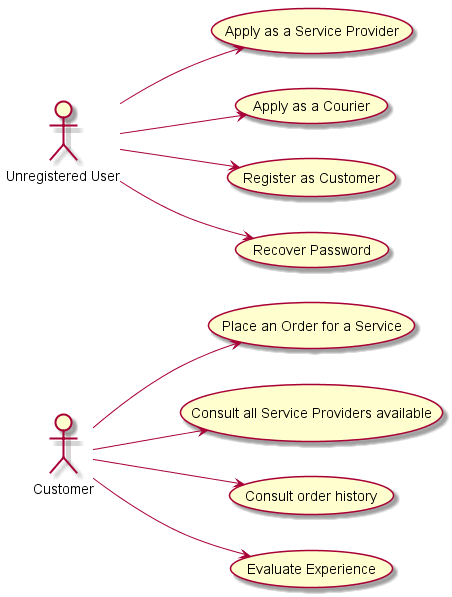
\includegraphics[width=\linewidth]{chapters/Requirements_Engineering/assets/FrontOfficeUseCaseDiagram.png}
\end{minipage}%
\begin{minipage}{.5\textwidth}
  \centering
  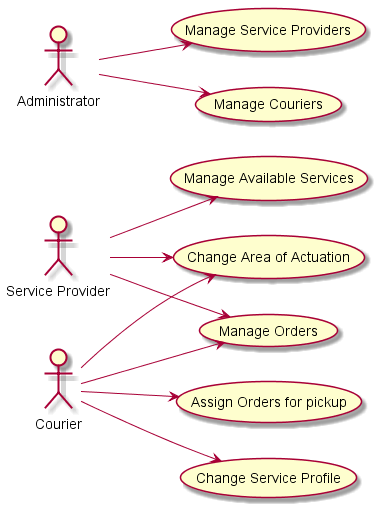
\includegraphics[width=\linewidth]{chapters/Requirements_Engineering/assets/BackOfficeUseCaseDiagram.png}
\end{minipage}
\caption[Use Case Diagram]{Use Case diagram}
\label{fig:useCaseDiagram}
\end{figure}

\par

Considering that there will be different responsibilities for the users of this platform, there is a need to define what are they and which user groups do the define. Hereupon, the main users of the platform will be:

\begin{itemize}
    \item \textbf{Unregistered User} - A user who has just reached the platform. Hasn't authenticated yet;
    \item \textbf{Customer} - A user which is a customer and is in look of a service;
    \item \textbf{Courier} - A user which is a courier and will be the people which will make the transportation of the necessary goods and materials associated to a service;
    \item \textbf{Service Provider} - A user which is a service provider and will be the responsible to provide the service requested by the customer;
    \item \textbf{Administrator} - The administrator of the platform. Responsible to manage service providers, couriers and the platform as a whole. 
\end{itemize}
\par


\par
The figure \ref{fig:useCaseDiagram} presents a use case diagram where it is possible to see all the actors and the functionalities that each one can access. On the left side there are the actors which access the core front-office functionalities such as placing an order or register. These actors are the customer and an unregistered user. On the right side we have the management and back-office actors that are responsible for the operational side of the platform. The actors for these actions are the service provider, the courier and the platform administrator.

\section{Functional Requirements}
\label{sec:functional-requirements}
In this section, the functional requirements of the system will be presented. Each of the requirements will then be split in smaller user stories throughout the project.

\subsection{FF01 - Register as Customer}
\textbf{User Groups}: Unregistered User

\subsubsection{Requirement Description}
Besides being able to consult some marketing material and information about the platform, the most common action that an unregistered user can make is registering. If the user chooses to register as a customer, some data will be needed to make it happen. The mandatory information for the registration be successful are: 
\begin{itemize}
    \item Name
    \item E-Mail
    \item Password
\end{itemize}

The user may complement with other information (address, phone contact, edit information) in the “My account” page.
\par
After the registration, an email will be sent to confirm the email address. In that email, there will be an url for the confirmation. While the account has not been activated, no orders may be done.


\subsection{FF02 - Apply as a Service Provider}
\textbf{User Groups}: Unregistered User

\subsubsection{Requirement Description}
An unregistered user may also choose to apply as a service provider. In this case, some data will be needed to make it happen. The mandatory information for the registration be successful are: 
\begin{itemize}
    \item Name of the service provider
    \item Name of the representative
    \item Address
    \item Service type (Laundry, mechanics, warranty...)
    \item Area of Actuation (Coordinates of the location of the service provider and the desired radius)
    \item Email
    \item Password
\end{itemize}

The user may complement with other information (phone contact, edit information) in the “My account” page.
\par
After the registration, this application for service provider will be sent to the platform administrators which will evaluate the viability of the \gls{SP}. In a first version, the management of the applications for service provider is not in the scope of this project. 
\par
The service provider will only be available in the platform after the administrator’s approval.

\subsection{FF03 - Apply as a Courier}
\textbf{User Groups}: Unregistered User

\subsubsection{Requirement Description}
An unregistered user may also choose to apply as a courier. In this case, some data will be needed to make it happen. The mandatory information for the registration be successful are: 
\begin{itemize}
    \item Name
    \item Profile type (motorcycle, van, car, etc.)
    \item Area of Actuation
    \item Email
    \item Password
\end{itemize}

\par
After the registration, this application for courier will be sent to the platform administrators which will evaluate the viability of the courier. In a first version, the management of the applications for courier is not in the scope of this project. 
\par
The courier will only be available in the platform after the administrator’s approval.



\subsection{FF04 - Log In}
\textbf{User Groups}: Unregistered User

\subsubsection{Requirement Description}
In order to authenticate before the platform, the unregistered user needs to log into an account. This is done with the email and password set upon the registration. If the password was changed after the registration, the latest password must be used.

\subsection{FF05 - Recover Password}
\textbf{User Groups}: Unregistered User

\subsubsection{Requirement Description}
In case of a lost/stolen password, an user may request for a password restore. To do this, the user must provide the email associated to the account and an email will be sent with a link to restore the password.

\subsection{FF06 - Place an order for a service}
\textbf{User Groups}: Customer

\subsubsection{Requirement Description}
When a customer selects a service that he/she desires, it will trigger the main process of the platform. Starting on the \gls{SDP}, the user needs to input some information regarding the service itself (in case of laundry, the platform will need information about the size of the size of the article, among others). After filling up all information regarding the selected service, the customer will be taken to the checkout page. In the checkout page, the customer will need to fill more information:
\begin{itemize}
    \item Pickup address
    \item Delivery address
    \item Billing address
    \item Preferred pickup hours
    \item Preferred delivery hours
\end{itemize}

After filling up all the information, the customer will be led to the payment page where he/she will select one of the existing payment options. This process will be done by a third party.
\par 
When the payment is completed, the order will be registered in back-office, an email with the order confirmation will be sent to the customer, and the order will be available to be consulted to the customer, the service provider that was selected and the couriers, to assign the orders.
At this point, the customer also needs to print the shipping guide, that will follow the article to the article.


\subsection{FF07 - Check all available service providers}
\textbf{User Groups}: Customers, Unregistered User

\subsubsection{Requirement Description}
When entering the platform web page, the customer (registered or not) will be able to check all the existing service providers and their services. All the services will be presented under its service provider on the \gls{SLP}. On this page, only basic information will be shown, as a description of the service and an estimate of prices.

\subsection{FF08 - Check order history}
\textbf{User Groups}: Customers

\subsubsection{Requirement Description}
The customer will be able to check their order history. This menu will be available as a tab of the “My Account” page.
\par
This page will show all orders made, date, and status (check section \ref{sub:order-states} for more information regarding the order states). The customer can also open the orders to get more information of what was ordered.


\subsection{FF09 - Evaluate Experience}
\textbf{User Groups}: Customers

\subsubsection{Requirement Description}
Every service provider will have a rating, depending on the performance for each service. This rating will be made by the customer after each order. The customer will need to rate some aspects regarding their experience with the platform, the service provider and the courier. In the first version, only service providers will have a rating. The customer will need to answer questions (classify 0-10) as:
\begin{itemize}
    \item How was your experience regarding the order process?
    \item Did the Service Provider fulfill your expectations?
    \item What about the experience with the courier?
\end{itemize}

\subsection{FF10 - Manage available services}
\textbf{User Groups}: Service Providers

\subsubsection{Requirement Description}
As the platform's service providers’ business grows, so will grow the offering of services available. This menu allows the service providers to create new, change and delete existent services. To be noted that a change of a service will actually create a new one, in order for the current orders for that service don't be changed.

\subsection{FF11 - Manage orders}
\textbf{User Groups}: Service Providers, Couriers

\subsubsection{Requirement Description}
In this menu, the service provider will be able to check all orders (current and past) and move them between a series of steps:
\begin{enumerate}
    \item New
    \item Picked on customer address
    \item Delivered to Service Provider
    \item Service Started
    \item Service Finished
    \item Picked on Service Provider Address
    \item Delivered to Customer
    \item Canceled
\end{enumerate}

The section \ref{sub:order-states} provides further information regarding the order states and its transitions.
\par
If the shipping guide is lost for some reason, the service provider can also print that document.

\clearpage
\subsection{FF12 - Change Area of Actuation}
\textbf{User Groups}: Service Providers, Couriers

\subsubsection{Requirement Description}
Both the couriers and service providers will need to select the \gls{AoA}. Only customers within this area of actuation will be able to select the services of the service provider in question. Likewise, couriers also need to select an area where they can make transportation. For an order to be fulfilled, there needs to be a courier that has both the customer and the service provider in their \gls{AoA}.

\subsection{FF13 - Change service profile}
\textbf{User Groups}: Couriers

\subsubsection{Requirement Description}
There may be services that require different kinds of vehicle for the goods to be transported. In this menu, the courier can change his vehicle type. There will be three options:
\begin{itemize}
    \item Scooter
    \item Car
    \item Van
\end{itemize}

In this case, a Van can transport any kind of goods, and a scooter will only be able to transport small goods.


\subsection{FF14 - Assign orders for pickup}
\textbf{User Groups}: Couriers

\subsubsection{Requirement Description}
The courier will be presented all the unassigned orders of in the defined \gls{AoA}. Here, the courier will be able to assign himself to the orders, meaning that he/she accepts to make the transportation and picking up the goods the schedule requested by the customer. When this assign is done, an email notification is sent to the courier’s email and the customer as well.

\clearpage
\subsection{FF15 - Manage Service Providers}
\textbf{User Groups}: Administrators

\subsubsection{Requirement Description}
In this menu, the platform administrators will be able to create, remove and consult information about the existing Service Providers.

\subsection{FF16 - Manage Couriers}
\textbf{User Groups}: Administrators

\subsubsection{Requirement Description}
In this menu, the platform administrators will be able to create, remove and consult information about the existing Couriers.

\section{Non-Functional Requirements}
\label{sec:non-functional-requirements}
In the previous section, the functional requirements were identified. Those requirements help to understand \textbf{what} the application will do. On the other hand, non-functional requirements specify \textbf{how} the application will do it. 
\par
In this section, an overview will be given regarding these requirements. They are to be considered throughout the development of the features identified in the section \ref{sec:functional-requirements}.

\subsection{Usability}
The system needs to be accessible from anywhere. This means that web apps need to be responsive for users being able to access it from mobile devices.

\subsection{Security}

The SnapTasks Portal is the one which will be responsible for managing the order requests and by consequence, it will also be responsible for managing the payments. It is mandatory to ensure the security of the payments, to diminish fraudulent orders. 
\par
To avoid man-in-the-middle attacks, all communications between services must be done using HTTPS.
\par
All personal data must be handled taking into account the current legislation.
\par
The system as a whole must have, at least, basic security systems, as:
\begin{itemize}
    \item \textbf{Authentication:} the system must be sure of who is making a certain request. This can be managed using username/password login;
    \item \textbf{Authorization:} the system must ensure that whoever is making a certain request, has permissions to do so. This can be managed by assigning roles to users, where a role grants access to a number of functionalities.
\end{itemize}

\subsection{Availability}
The SnapTasks Portal must have the minimum downtime possible, for not losing customers because of having the website down.
The back-office tools should also be down the least time possible. However, this scenario has a lighter impact, since the customers are still able to access the portal and place orders.

\subsection{Scalability}
The delivered solution must be capable to be scaled dynamically. This means that the access of many different users at the same time does not affect the website performance. 
\par
To attain this, a cloud service, such as \textit{Azure} is to be used, allowing to increase and decrease the hardware resources depending on the needs.

\subsection{Resilience}
The platform must be resilient to handle wrong input from the users or sudden failures of dependent services. 
\par 
Those errors should be handled and the user who has made the request should be informed about what happened. 

\subsection{Performance}
The system must be fast and efficient in order not to lose a customer because the application was not responding. For this to happen, most of the processing should be done in back-office, using asynchronous processes.
\par
This requirement will be more important as the platform has more users. 

\par

\subsection{Internationalization and Localization}
The platform will be used firstly in Portugal, therefore, it should have its front-office in Portuguese.
\par
However, as the platform grows, there may be the need to have SnapTasks Portal in different languages and cultures. The application should be prepared for that case.

\subsection{Maintainability}
The platform code should be easy to maintain. This means that both bug fixing and adding new features should be as easy as possible, following the industry's best practices.

\section{Process View}
To have a better understanding of how the whole platform will work, we need to have a clear view of the operational process which this system supports. This can be achieved by analyzing the flow that an order takes, since it is placed until the service is finished and all goods are returned to the customer.
\par
It starts when a registered customer accesses the system. He/she will select a service he/she needs, proceed to checkout, make the payment and place the order. At this point, the order is created in the system and can be accessed by the courier to assign himself, compromising to make the delivery from the customer's pickup address to the service provider address. This assignment is only for the first leg of this order (from the customer to the \gls{SP}). At the date selected by the customer, the courier will go to the customer's address to pickup the goods associated to the order and then deliver them to the service provider. The service provider now has the goods and is ready perform the ordered service. After the service is finished, the order status is changed to \textit{Service Finished}, allowing the couriers to know that the goods associated to that order are ready to be returned to the customer. Therefore, they also can assign themselves to that transportation, compromising that they will do the second leg of the order (from the \gls{SP} to the customer). In this case, the goods can be picked up at any time, because the service provider has an open store. After picking up the goods at the \gls{SP}'s address, the courier will deliver the items to the customer, finishing the process.
\par

The figure \ref{fig:processDiagram} presents a more graphical view of this process and shows how the user groups interact.

\begin{figure}[ht]
\centering
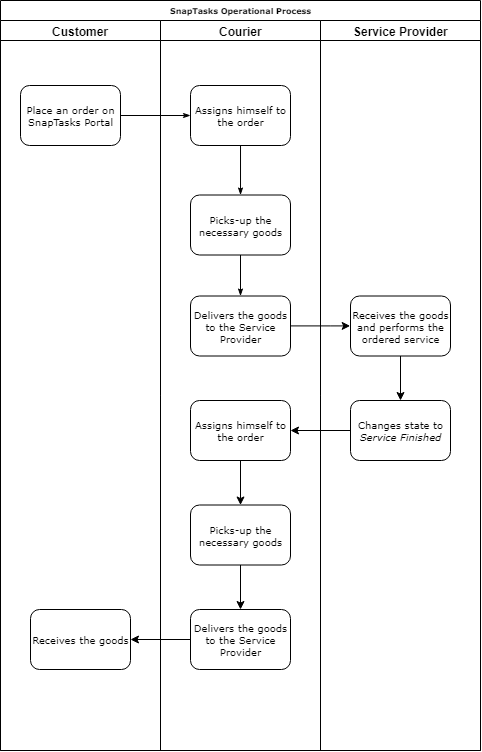
\includegraphics[width=0.98\textwidth,keepaspectratio]{chapters/Requirements_Engineering/assets/ProcessDiagram.png}
\caption[Process diagram]{Process diagram}
\label{fig:processDiagram}
\end{figure}

\clearpage

\section{Order Process States}
\label{sub:order-states}

In the previous section, it was possible to understand that the order goes through several steps for the service to be fulfilled. These steps are represented by the states in which an order can be.
Each state represents something that is occurring/occurred, or an action that is needed.
\par
The possible states for a given order are the following:

\begin{itemize}
    \item New;
    \item Picked on customer address;
    \item Delivered to Service Provider;
    \item Service Started;
    \item Service Finished;
    \item Picked on Service Provider Address;
    \item Delivered to Customer;
    \item Canceled.
\end{itemize}

These states reflect the operational status. Each order must go through these states sequentially. For example, an order cannot be delivered to the customer before the service is finished, or, an order's service cannot start before the goods are delivered to the service provider.
\par
The figure \ref{fig:orderStateDiagram} shows how the order states connect to each other and represents the happy path workflow.

\begin{figure}[ht]
\centering
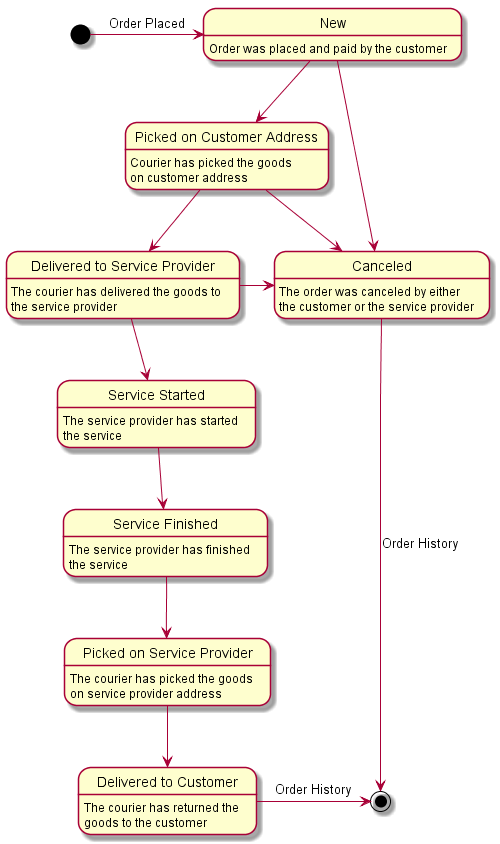
\includegraphics[width=0.91\textwidth,keepaspectratio]{chapters/Requirements_Engineering/assets/StateDiagram.png}
\caption[Order State diagram]{Order State diagram}
\label{fig:orderStateDiagram}
\end{figure}

\chapter{Analysis of the Existent Solutions} % Main chapter title
\label{chap:existent_solutions_comparison}
After the identification of the functional and non-functional requirements of this project, in the previous chapter, it is necessary to have a better understanding about which of the architectures and technologies, identified in the section \ref{sec:StateOfTheArt_Technology}, are the best choice to be used in the context of this dissertation. It is important to perceive the difference between each of them and compare its pros and cons. In this chapter, the advantages and disadvantages of using each of the technologies or architectures in the context of the project of this thesis.


\section{Architectural Approaches}
\label{sub:architectural_approaches}
The first topic to be discussed, is also one of the first topic to discuss when developing a new project from scratch. The architecture of a system is like the skeleton a human being. It sustains the whole body while actually doing nothing by itself. A clear definition of the architecture that will be used in the system may prevent many problems since it provides a clear vision of the system as a whole. 
\par
In the section \ref{sub:StateOfTheArt_Technology_Architecture}, a few architectures were presented to the reader. In this section, the best and the worst of each of the architectures will be presented and then compared using \gls{CBAM}. Developed by the \gls{SEI}, this method is an "architecture-centric method for analyzing the costs, benefits and schedule implications of architectural decisions" \parencite{scenarioBasedArchEvaluation}.

\subsection{Micro-Services}
Micro-services, as was already mentioned in section \ref{sub:StateOfTheArt_Architectures_microservices}, micro-services architecture is a architectural style where applications are broken in autonomous "small pieces", the so called services, with a very well defined responsibility. 
\par
One of the biggest advantages of the micro-services architecture is that each service is independent of the others. It is possible to scale or deploy just one service at a time without affecting the others. This facilitates the development because, since the services are independent of each other, they can be developed in different languages. However, the communication protocol must remain the common. This makes the service more targeted to what is its responsibility. All this makes the system more robust as a whole. As the services are loosely coupled, if one services fails, only the functionalists that need that particular service will be affected as opposed to the monolithic, where if anything fails, everything fails. Lastly, it is easier to coordinate the development with several teams when the system uses a micro-services architecture, since every development will be localized in a single application and there will be less conflicts when merging code \parencite{microservicesProsAndCons}.
\par
On the other hand, if the initial definition of the responsibility is not well defined, it is much harder to make a structural refactor on a system with this architecture than it is with a monolith. Besides, any interface changes need to be coordinated with the teams that work on the other services. The benefit of being able to deploy independently creates another problem. There needs to be a deployment process for each application. If each service has the need to have its own deployment process, this can affect the complexity of maintaining that process. Testing may also be another problem. If the service is being tested has dependencies of other services, it may be difficult to test it. Either the service has correct data to be accessed directly, or the dependencies are mocked. Finally, as the communication between service is made through the network, this may affect the overall performance of the system \parencite{microservicesProsAndCons}.

As micro-services are a part of \gls{SOA}, the analysis will be kept in this more specific architecture. 

\subsection{Event Sourcing}
As was already mentioned in section \ref{sub:StateOfTheArt_Architecture_EventSourcing}, Event Sourcing is an architectural pattern where every change on an entity, generates and persists an event. This event will be listened by the interested parties which will or will not do something about it, as its logic dictates.
\par
The best thing about this pattern is the preservation of the state history. This element is very useful for certain businesses as banks, where every change may be audited. In Event Sourcing, every change in the state of an entity is kept in record. Using an event driver to communicate asynchronously between services offers a extremely loosely coupled alternative to the traditional \gls{HTTP} requests, since in this case, the service doesn't even know about the existence of the service where it is getting information from \parencite{eventDrivenArchitectureOverview}. In case a business process needs to do several things in response to a change on an entity, the responsibility to trigger those actions are no longer in the source of that change, but on the services that are listening the event. They are the ones responsible to take (or not) action over a certain event.
\par
Nonetheless, as it is true for every pattern, this approach also brings problems. Tools for development are still rare and as it is a relatively new alternative, there are not many use cases to take as an example \parencite{prosAndConsEventSourcing}. Also, for development environment, this requires all services that have dependencies to be synchronized, which may bring problems for integration tests.

\subsection{CQRS}
In a nutshell, \gls{CQRS} is a pattern that segregates the reads and the writes into two different components. This is explained in more detail in section \ref{sub:StateOfTheArt_Architecture_CQRS}.
\par 

\gls{CQRS} offers great benefits for systems that have a big discrepancy between the number of reads and writes, since, as they are separate components of the system, they can be scaled independently, offering a bigger flexibility to the system. In case of a big concurrency happening in the system, it is also possible to optimize each component for the action that they perform. Also, it offers the possibility to have different representations for read and write operations.

However, using \gls{CQRS} pattern offers several risks. The use of different models may cause inconsistency problems between them. This inconsistency is even bigger for systems that have a big overlap between reads and updates, which is true for most applications. If the application doesn't have a lot of traffic to handle, the usage o \gls{CQRS} may bring more problems than benefits. As this platform is expected to grow, and to have its traffic increasing over time, this is something that may bring some problems. 

\par 
Its complexity is considerable and it is focused in a specific problem to be solved.

\subsection{Summary}
\label{sub:ExistentSolutions_Architecture_Summary}
In the previous points, several benefits and risks were presented regarding each of the possible architectures. The table \ref{tab:Sumary_evaluation_architectures} presents a summary of the relevant pros and cons of each one.

\par


\begin{table}[ht]
\caption{Summary of Pros and Cons of each evaluated architecture}
\label{tab:Sumary_evaluation_architectures}
\resizebox{\textwidth}{!}{%
\begin{tabular}{|l|l|l|}
\hline
\textbf{Architecture} & \textbf{Pros}                                                                                                                                                      & \textbf{Cons}                                                                                                                                                                                   \\ \hline
\textbf{Micro-Services}                       & \begin{tabular}[c]{@{}l@{}}Services are Independent\\ Different languages are supported\\ Low coupling\\ Resilience\\ Easy coordination between teams\end{tabular} & \begin{tabular}[c]{@{}l@{}}Need for a clear definition of each service\\ Interface changes need to be coordinated\\ Many deployment processes\\ Testing dependencies\\ Performance\end{tabular} \\ \hline
\textbf{Event Sourcing}                       & \begin{tabular}[c]{@{}l@{}}State history persistence\\ Extremely low coupling\\ Event triggers all needed processes\end{tabular}                                   & \begin{tabular}[c]{@{}l@{}}Few use cases implemented\\ All dependencies must be synchronized for tests\end{tabular}                                                                             \\ \hline
\textbf{CQRS}                                 & \begin{tabular}[c]{@{}l@{}}Flexibility on reads/writes\\ Independent scaling and optimization\\ Different representations for reads and writes\end{tabular}        & \begin{tabular}[c]{@{}l@{}}Possible inconsistency problems\\ Complexity\end{tabular}                                                                                                            \\ \hline
\end{tabular}%
}
\end{table}
\par

Considering the project of this thesis, it was decided, all things considered, to go with the micro-services approach. This decision was based on the wide number of use cases that exist for this architectural style, its proved resilience, which is also a non-functional requirement of this project (check section \ref{sec:non-functional-requirements}). Since there is no requirement for an extremely low coupling and independent scaling between read and write operations, the complexity of \gls{CQRS} and the risk of implementing an architecture with fewer use cases implemented as event sourcing, don't compensate the pros of these architectures, meaning that they are not the best option for the problem we are trying to solve.


\section{Software Development Frameworks}
The purpose of using a Software Development Framework is to have, right out of the box, a series of tools, abstractions and libraries that help on the development process. It is very important to use a framework that fulfils the needs of the project and facilitates its implementation.
\par
In the next sections, several possibilities will be analyzed in order to correctly understand which one fits this project the best. The approach to do this will be similar to what was done in the section \ref{sub:architectural_approaches}, weighing the pros and cons of each one.

\subsection{.NET Core}
.NET Core, as explained in section \ref{sub:StateOfTheArt_Frameworks_NET}, is a cross-platform software framework that provides several tools to create applications for different purposes. 
\par
In this project, we aim to develop an e-commerce platform that provides different functionalities for logistics in service provision. Since this framework allows the creation of both \gls{API}s and web applications, it means that it is possible to develop the project in this framework. 
\par
The fact of being cross-platform, means that the costs can be reduced since the services can run on Linux, which is a cheaper option when compared to Windows Server. This framework also provides a seamless integration with azure which enables the deploy of services directly from Visual Studio. 
\par
The automatic monitoring saves us the time of having to implement the basic monitoring features such as response time, application exceptions and throughput.
\par

Regarding the issues of this framework (also identified in section \ref{sub:StateOfTheArt_Frameworks_NET}) holds on the licensing costs for the usage of some functionalities in Visual Studio, the low flexibility o Entity Framework, and the fact that Microsoft technology depends a lot on the company's decisions. 
\par 
Taking into account that this is an academic project, the existence of academic licenses removes the first issue. On the other hand, the other two cons are still unsolved.

\subsection{Java Spring}
As presented in section \ref{sub:StateOfTheArt_Frameworks_java}, Java Spring is an open-source software framework that, similarly to .NET Core, allows the development of both web applications and \gls{API}s. Since these are the essential application types of this project, it is also possible to be developed using this framework
\par
Java Spring is a very flexible framework that provides tools for several cross-cutting concerns, such authentication, authorization and logging. It also provides support for \gls{AOP}, which enables the implementation of those cross-cutting concerns in a clean way.
\par
However, this framework has a high learning curve due to the large number of classes and tools that the developers need to know to develop efficiently, which can make the project more complex which, consequentially, makes the development to take longer. Additionally, there is a lack of security guidelines, as was already mentioned in the section \ref{sub:StateOfTheArt_Frameworks_java}. 

\par

Considering the nature of the project (e-commerce and with a fixed delivery date), these cons are very difficult to overcome.



\subsection{Node.js}
Node.js is a software framework that was designed for applications that require real-time updated data, such as video-conference rooms or online gaming, as mentioned in section \ref{sub:StateOfTheArt_Frameworks_Node}. As the last two frameworks, it also allows the development of both \gls{API}s and web applications, which allows the project to be developed in this framework. 
\par
This is a very lightweight framework, since it uses non-blocking, event-driven I/O, that provides tools to build fast and scalable applications. It uses JavaScript as its development language, which keeps the learning curve to a minimum for a team that already has to use JavaScript in the front-end, since this language is largely used for front-end purposes.
\par
However, since this framework is largely developed by the community, there are many tools that are of poor quality, specially in non-core modules. Also, as Node.js is single threaded, it is not indicated for applications that require heavy \gls{CPU} operations.
\par
As this project does not have any requirement regarding real-time data, the biggest advantage of using Node.js ends up having no use. The low learning curve is also a pro that does not apply to our case, since no one in the development team has experience in JavaScript 


\subsection{Summary}
In the previous sections, the pros and cons of each framework and its viability for this project were analyzed. The table \ref{tab:summary_Frameworks} presents a summary of the relevant benefits and risks of each one.
\par

\par
For the project of this dissertation, and taking into account the benefits and risks of the three evaluated frameworks, it was decided to go for the .NET Core framework. This decision was mainly for the cross-platform possibility and its reliability. As the main cons are concerning licensing costs and there are student licenses available for free, the downside of this framework is fairly reduced.
\par
When compared to the Java Spring, the main problem is the Spring high complexity and learning curve. Also, the lack of security guidelines for this framework is a threat for an e-commerce platform, as this project is. With the existent deadlines, the benefits of this framework doesn't pay off the risks.
\par
In the case of Node, its lightweight and fit for micro-services architectures would be a great plus. However, with the problems of the existent tools, and the unfamiliarity by the development team of this technology, it was understood, that .NET Core would be a better fit.


\begin{table}[hb]
\caption{Summary of Pros and Cons of each evaluated software development framework}
\label{tab:summary_Frameworks}
\resizebox{\textwidth}{!}{%
\begin{tabular}{|l|l|l|}
\hline
\textbf{Framework} & \textbf{Pros}                                                                                                                          & \textbf{Cons}                                                                                                                                \\ \hline
\textbf{.NET Core}                         & \begin{tabular}[c]{@{}l@{}}Cross-platform\\ Development in Visual Studio\\ Multi-Language\\ Automatic Monitoring\end{tabular}          & \begin{tabular}[c]{@{}l@{}}Licensing Costs\\ Low flexibility of Entity Framework\\ Dependency on Microsoft\end{tabular}                      \\ \hline
\textbf{Java Spring}                       & \begin{tabular}[c]{@{}l@{}}Flexibility\\ Support for AOP\\ Provides several useful libraries\end{tabular}                              & \begin{tabular}[c]{@{}l@{}}High learning curve\\ Complexity\\ Lack of security guidelines\end{tabular}                                       \\ \hline
\textbf{Node.js}                           & \begin{tabular}[c]{@{}l@{}}Lightweight\\ Same language as front-end\\ Low learning curve\\ Good option for micro-services\end{tabular} & \begin{tabular}[c]{@{}l@{}}Many tools are of poor quality\\ Callback hell\\ Single-thread\\ Quality of code on non-core modules\end{tabular} \\ \hline
\end{tabular}%
}
\end{table}



\chapter{Design and Architecture} % Main chapter title
\label{chap:Chapter5} 
The importance of a correct architecture was already mentioned in the sections \ref{sub:StateOfTheArt_Technology_Architecture} and \ref{sub:architectural_approaches}. For that reason, in this chapter, we will start with an architectural study, where the bet architecture for the system was thought and designed. Although the architecture of a system is a very important step while designing a system, the inner design of the component must not be forgotten. That design will also be presented in this chapter. Furthermore, the domain model of the platform, will also be presented.

%----------------------------------------------------------------------------------------
\section{Architectural Study}
\label{sub:architectural-study} 
In order to have the most correct architecture for the platform in analysis in this dissertation, a study took place, where the system as a whole was examined to see how it would be possible to model an architecture that would fit our system. The name of the platform is SnapTasks.
\par
The first step was to identify how many different front-end applications the system would need. This was done taking into account the existent users groups that exist and their needs. As it was already presented in section \ref{sec:Requirements_userGroups}, there are four main actors: the final customers, the service providers, the courier and, finally, the administrators. The decision of what applications to have was mostly based on the actors that exist, and their needs.
\par

These will be the client applications of the platform: 
\begin{itemize}
  \item \textbf{SnapTasks Website}: the main website of the platform. This is where the users will create their accounts, customers will place their orders and know the available services;
  \item \textbf{\gls{BO} Management}: this application will be responsible for all \gls{BO} and administration operations. Service providers will track their orders in this application;
  \item \textbf{SnapTasks Mobile Application}: similarly to the main website, this will provide essentially the same functions, but on a mobile Android app. Taking into account the graph in figure \ref{fig:mobileGrowth}, it is almost mandatory to have a mobile application, from the beginning;
  \item \textbf{Courier App}: this application allows couriers to check the orders that need pickup and assign themselves to them. This application will also provide the location where the courier needs to pickup/delivery and integrate with the \gls{GPS}.
\end{itemize}

\par
As these applications will be mandatory in our application, one possible architecture would be to keep things to a minimum and have only one \gls{API} that would be responsible to provide all the necessary functionalities to the client apps. Furthermore, it would also be needed a database to persist all the data. Having the minimum number of components means that, in short-term, there will be less development work, the monitoring will also be easier \parencite{monolithProsAndCons}. This architecture is presented in figure \ref{fig:monolithProposal}. 
\par

\begin{figure}[ht]
\centering
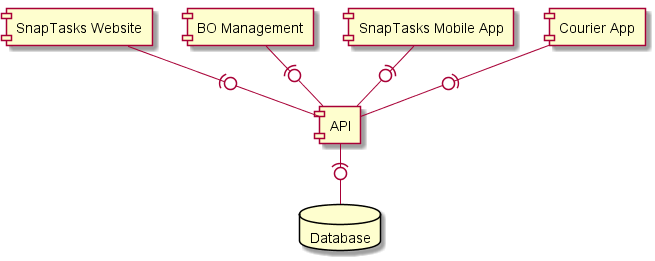
\includegraphics[width=\textwidth,keepaspectratio]{chapters/Architectural_Overview/assets/Monolith.png}
\caption[Possible architectural solution (Monolith)]{Possible architectural solution (Monolith)}
\label{fig:monolithProposal}
\end{figure}

\par

These architectures are known as monolith. This is because all the logic of the system is centred in a single component, without any rule. Monolithic architectures bring more evil than good. With every logic located in the same place, the code can easily become tightly coupled and become very hard to read \parencite{monolithAreBadDesign}. On a logical thinking, it doesn't make sense to provide functions that a certain application will never need. 
\par
In the proposal presented in the figure \ref{fig:monolithProposal}, this happens with the \gls{FO} and \gls{BO} applications. Since each application type needs very different kinds of functionalities. The first ones will need more customer focused operations such as get the available services and placing an order. The second ones need more operational functionalities, like managing service providers or add more services to the platform. 
\par
For that reason, it was decided to split the \gls{API} into two different ones. The first for front-office operations and the second for back-office operations. In this solution, it is possible to segregate the functionalities and restrict its access to the applications that actually, need them. The figure \ref{fig:foBoSeparation} presents an illustration of the possible separation of these functionalities.

\begin{figure}[!hb]
\centering
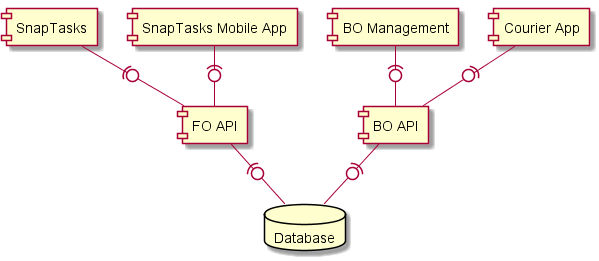
\includegraphics[width=0.9\textwidth,keepaspectratio]{chapters/Architectural_Overview/assets/BoFoSepartion.png}
\caption[Separation of FO and BO APIs]{Separation of FO and BO APIs}
\label{fig:foBoSeparation}
\end{figure}

\par
In this architecture, the separation of allowed not only to separate the concerns of each \gls{API}, but also, to have less load on the services. In case of an unexpected increase of orders, it is possible to temporarily boost the resources of just the FO API, instead of having to upgrade the whole system.
\par
On the other hand, as the application is expected to grow both in terms of number of functionalities and in terms of load, it would be better to have the code even more segmented and decoupled. To achieve this, and as was already explained on section \ref{sub:ExistentSolutions_Architecture_Summary}, a micro-services architecture was designed. 
\par
To design this architecture, it was needed to identify which services were needed and what was their responsibility. From that analysis, the following services were identified: 

\begin{itemize}
  \item \textbf{Pricing Service}: this service is responsible for the creation, calculation and get operations of prices. Each new price that is entered will create a new registry on the database, in order to keep track of the prices and provide a link of the prices that were used in the orders;
  \item \textbf{Order Management Service}: this service is responsible for all the operations that concern the orders. This includes the overall management (create, update), transitions between steps and other logic that is inherent to this entity;
  \item \textbf{Service Provider Management Service}: similarly, this service is responsible for the operations that regard both the service providers and their services. Management operations like create, deactivate and update are under the scope of this service;
  \item \textbf{Courier Service}: the last service is relative to the couriers. Following the previous logic, this service is also responsible to manage the couriers and provide operations that regard the couriers.
\end{itemize}

\par
All services will be bellow both FO API and BO API, which means that those APIs can access the services, but the services can't access the APIs. Furthermore, as the services are only responsible to make operations that only affect the entity in question, there should be no reason for a micro-service to access another micro-service. Lastly, each service is provided a database and the service is responsible to manage it. No service can access the database of another service. The figure \ref{fig:microservicesProposal} presents the proposed architecture.
\par

\begin{figure}[ht]
\centering
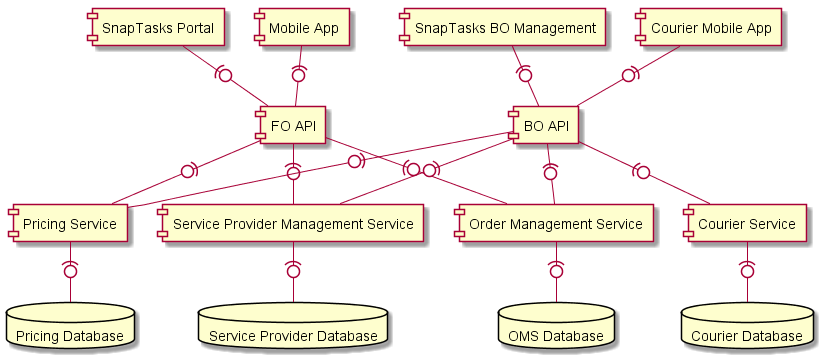
\includegraphics[width=\textwidth,keepaspectratio]{chapters/Architectural_Overview/assets/MicroServices.png}
\caption[Proposal of a Micro-Services Architecture]{Proposal of a Micro-Services Architecture}
\label{fig:microservicesProposal}
\end{figure}


\section{Domain Model}
\label{sec:Implementation_DomainModel}
The design of the domain model is one of the most critical phases in software engineering. This phase not only allows the team to have a better understanding of the business that the application is contained, by helping to identify key concepts and ideas of the business domain, but can also serve as a baseline for the development of a new solution. The domain model is a visual representation of the entities that concern the problem that our application is trying to solve.

\par

With the purpose of having a better understanding of the problem it is being aimed to solve, a domain model was designed. This domain model presents the main concepts and entities that are present in the domain. The figure \ref{fig:domainModel} represents the visual component of the most important concepts on the business domain.



\par
With this visual representation of concepts, it's easier to understand what are the key entities that concern the problem. However, there is still a need to deep dive into these concepts to know what they represent.

\par

The \textbf{order} is one of the most central concepts in the diagram because it is one of the most crucial components of the solution. The whole purpose of the platform is to create and process orders. They are placed by the final \textbf{customer} by interacting with the platform front-end. When the customer places his/her order, it is possible to define where and when he/she desires that the pickup of goods is to be made. This order also has a \textbf{cost}, which is the value that the customer paid for it, which includes both the value for each service, and the logistics fee, for the transportation of goods (including promocodes, if that is the case).
\par
The \textbf{service providers} are another fundamental part of the platform. They are the ones who provide the \textbf{services} that are available on the platform without whom, there would be no orders to be placed. The \gls{SP} also has a \textbf{representative}, which is the point of contact between the provider and the platform. To improve the service quality and avoid orders from customers who are too far away from the \gls{SP}, it is required for the service provider to define an \textbf{area of actuation}. This \gls{AoA} defines a circular area with its center in the \gls{SP}'s address, where it is possible to order from that service provider.
\par
The services that are provided can be of several \textbf{service types} (laundry, mechanics, warranty, etc.), however, for the first version of this application it will only allow laundry services. Nevertheless, the platform is prepared to provide any kind of services. The platform is also prepared to have multiple services gathered in a single order, but as an \gls{MVP}, only one service can be ordered in the front-end.
\par
Each service has its own \textbf{prices}. The price represents the breakdown of what the user will pay por a given service. 
\par

The goods that concern a given order are transported from the customer's and the service provider's \textbf{address} by the \textbf{courier}. This actor is also responsible to assign him/herself to the orders that he/she will deliver. The address contains the necessary information to reach the customer and the service provider, such as name, address info, zip code, city, etc.

\begin{figure}[ht]
\centering
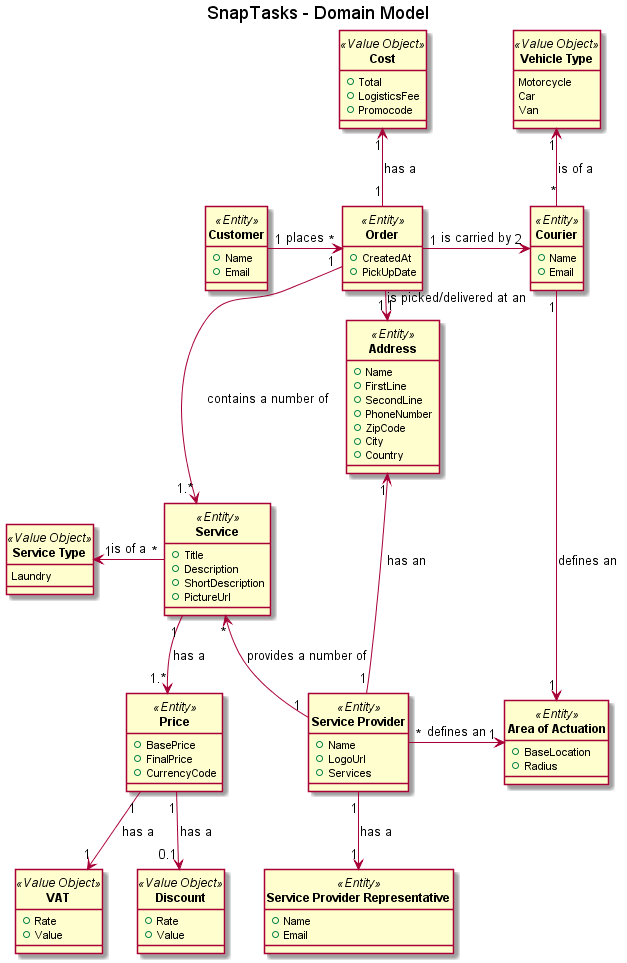
\includegraphics[width=\textwidth,keepaspectratio]{chapters/Architectural_Overview/assets/SnapTasks-DomainModel.png}
\caption[SnapTasks Domain Model]{Snaptasks Domain Model}
\label{fig:domainModel}
\end{figure}

\clearpage
\section{Internal Project Structure}
\label{sec:internal-project-structure}

In the section \ref{sub:architectural-study} the macro architecture of the solution was presented. On the other hand, the internal project structure of each component is still to be presented. The present section is the one where that will be done.

\par

For this solution, each component had an internal layer architecture. This is one of the most common architecture patterns in the industry, and is also known as n-tier architecture pattern. This pattern organizes the application into horizontal layers, each one with its own responsibility, performing a specific role for the application. Despite the nonexistence of a rule for how many layers to exist in a given application, the standard consists in four layers: presentation, business, persistence and database \parencite{softwareArchitecturePatterns}.   

\par

The layered architecture pattern has as one of the most powerful features the separation of concerns among components. The components within a given layer will only need to deal with logic that is that layer's responsibility. For example, the components that are inside the business layer, will only need to deal with business logic. Same applies for the components of the persistence layer, which will only need to have persistence related logic. This makes the components' responsibility easy to define and, by consequence, makes it easier to develop, test and maintain them.

\par

The figure \ref{fig:internalProjectArchitecture} presents the generic layer structure used for the services that compose SnapTasks solution. Despite the layer structure being the same for all components, the biggest difference resides in the \textit{Data} layer. Given that only the bottom services have access to databases, only those services will have a \textit{Repository} and \textit{Database Object \gls{DBO}} sub-layer, since without the need to access a database, there is no need for repository logic and \gls{DBO}. Instead, those services will most likely need to access other services in order to retrieve data. That logic is contained in the \textit{Gateway}.

\par
\begin{figure}[ht]
\centering
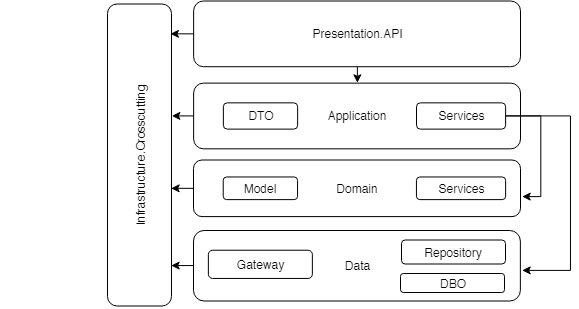
\includegraphics[width=\textwidth,keepaspectratio]{chapters/Implementation/assets/Internal-Service-Architecture.png}
\caption[Generic representation of the internal project structure]{Generic representation of the internal project structure}
\label{fig:internalProjectArchitecture}
\end{figure}

\subsection{Presentation}
\label{sub:InternalStructure_Presentation}
The top layer is named \textbf{Presentation.API} or \textbf{Presentation.Web}, depending if the component is an \gls{API} or an application with \gls{GUI} respectively, is responsible to handle the application's incoming requests. This layer is also responsible to ensure that the incoming data is valid to proceed to the next layer. When the application has a \gls{GUI}, this layer is also responsible to handle the user interaction with the interface. The figure \ref{fig:serviceListingPage}, of section \ref{sub:service-listing-page}, presents the \gls{SLP} of one \gls{SP}.

\par 
In the case of the \glspl{API}, it is possible to check the available endpoints in the \gls{API}'s Swagger page (more information about swagger on section \ref{sub:swagger}).


\subsection{Application}
\label{sub:implementation-application}
The second layer in the chain, \textit{Application}, is the one that is responsible for most of the business logic. This layer is divided into two sub-layers, \textbf{Application.Dto} and \textbf{Application.Services}. The first one is where the \glspl{DTO} are defined. The segregation of this to a separate package, allows to generate a \gls{DLL} that can be used by other projects that need to use this application's \glspl{DTO}. 
\par
The second sub-layer, is the one responsible for the business logic itself. The methods of this layer will be called by the presentation layer, retrieve data from the data layer below, apply the necessary logic and then retrieve it to the presentation layer.

\subsection{Domain}
The \textit{Domain} layer is the one where the domain-related logic is contained. It is divided into two separate sub-layers, \textbf{Domain.Model} where the domain model is specified, and \textbf{Domain.Services}, where domain-related logic (for example, logic that concerns only one object) are implemented. Most of these methods are implemented using as extension methods, and can be used as an extension of the object itself.

\subsection{Data}
The bottom layer is responsible to know where and how to get and persist data in order to the application to work properly. The \textit{Data} layer can be composed by the \textbf{Data.Repository} and \textbf{Data.Dbo}, when the application needs to access a database, and by a \textbf{Data.Gateway}, if it needs to access another application, being that application within the SnapTasks ecosystem, or not. 
\par
The \textit{Data.Dbo} sub-layer is where the \glspl{DBO} are defined. These objects are a representation of the database itself and are needed in order to the used \gls{ORM}, Entity Framework Core, to work properly. These objects are also used by the other sub-layer to access the database. In the \textit{Data.Repository}, all the logic needed to access the database is contained.

\par

In terms of the \textit{Data.Gateway}, it contains all the necessary logic needed to access an external service. As opposed to when we access a repository, we also have ownership of the \glspl{DBO} needed to access, when accessing an external service, that ownership belongs to the application we are calling. The \textit{Data.Gateway} needs to use the \glspl{DTO} provided by that service (also check section \ref{sub:implementation-application}).


\subsection{Infrastructure}

Last, but not least, there is the \textit{Infrastructure} layer. This layer is responsible for the crosscutting concerns that are required by all the other layers. That includes:
\begin{itemize}
    \item Logging
    \item Authorization
    \item Authentication
    \item Mappings
    \item Caching
\end{itemize}
\par

This layer ends up being slightly different from the others because it is not above or below any of the other layers. Instead, it is on the side, and may be accessed by any of the other layers. However, the \textit{Infrastructure} layer can not access any of the remaining layers of the project.
\chapter{Implementation} % Main chapter title
\label{chap:Implementation}

This chapter approaches the most technical component of this thesis. Here, it will be approached how the first version of the application was developed, considering both functional and non-functional requirements, defined in chapter \ref{chap:Requirements_Engineering}. Starting from how the code is structured in the different components, proceeding to the explanation of one of the main features of the project, the price calculation and how the code quality was measured. Finally, the application's user interfaces will be presented.

\section{Code Structure}
For the development of the project of this dissertation, the \gls{IDE} used was Visual Studio 2019. Each of the components identified in section \ref{sub:architectural-study} resulted in a solution in Visual Studio and, also, a different repository in the \gls{VCS}. In this case, the \gls{VCS} used was \textit{Git}.

\par

Inside the \gls{IDE}, the code was structured taking into account what was presented in section \ref{sec:internal-project-structure}. Each of the layers was mapped into a different \textit{Class Library} project. This allowed to have the code to be compiled separately which eases the management of dependencies between layers. After compilation, each project will result in a different \gls{DLL}. This allows for the compiled code to be used in different solutions by either having a direct reference to the compiled \gls{DLL}, or by creating a \textit{nuget} package and later installing it in the desired projects.
\par

The figure \ref{fig:vsProjects} presents the code structure on Visual Studio. For this example, the component used was the \textit{Order Management Service}.

\begin{figure}[!ht]
\centering
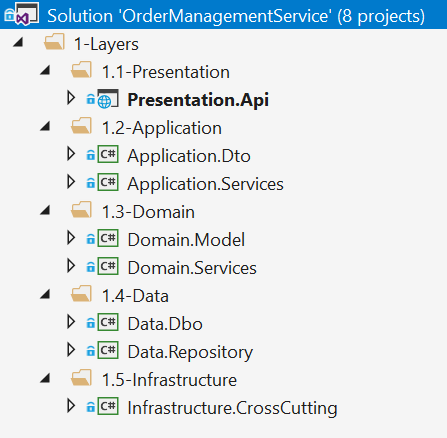
\includegraphics[width=0.8\textwidth,keepaspectratio]{chapters/Implementation/assets/vs-projects.PNG}
\caption[Code structure on Visual Studio]{Code structure on Visual Studio}
\label{fig:vsProjects}
\end{figure}

\section{Price Calculation}
The price calculation strategy is one of the most important components of an e-commerce website. It can be the thing that makes a customer come back to use the platform or, otherwise, it can be the thing that makes the customer to never come back. Furthermore, the calculation and breakdown of the price is also very important for law compliance. If, for example, the prices' \gls{VAT} parcel is not correctly calculated, the company may be paying less taxes than it should. This can result in fines that the company must pay, unnecessarily.

\par
 The price is an entity by itself rather than being a property of the service, as shown on figure \ref{fig:domainModel}. Each price has is immutable and have its own identifier. When an order is placed, this identifier is also persisted to keep a record of the price that was paid for each service. Also, this allows to have multiple prices for each service, if there is ever such a need. This is very useful for a use case where there are different prices for the same service, for example, with a \gls{VIP} customer segment, where customers in this segment have access to lower prices than a regular customer or have different prices for each country.

\par

On a technical level, when the user needs to update the price of a given service, the user makes that request to \textit{SnapTaks BO Management}, in the service details. This application uses BO API's endpoint to make the operation which afterwards makes a call to Pricing Service. This component is the one that contains all logic regarding prices and for that reason is where the logic for this operation is contained. The service will calculate the price, taking into account the \gls{VAT} and discount rates. If there is already a price in the database for the given service, that price will be disabled and the new price will be persisted as the price in use for that service.

\par

The sequence diagram in figure \ref{fig:priceUpdate} represents the update price flow between the several components of the platform.

\begin{figure}[ht]
\centering
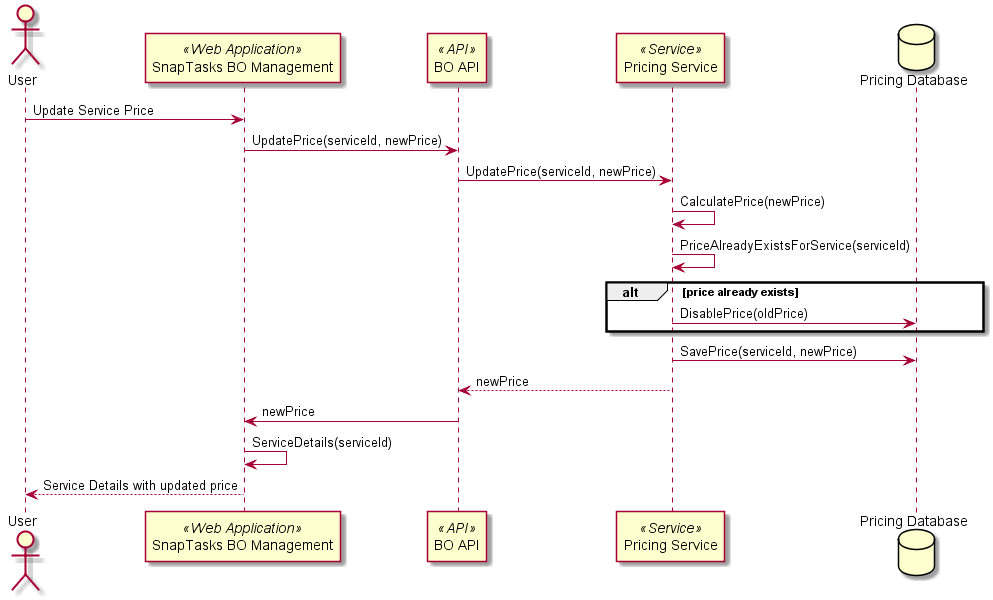
\includegraphics[width=\textwidth,keepaspectratio]{chapters/Implementation/assets/PriceUpdate.png}
\caption[Sequence diagram for price update]{Sequence diagram for price update}
\label{fig:priceUpdate}
\end{figure}

\par
The price composed by the \textbf{base price} and \textbf{final price}. The first one is the price that is defined by the \gls{SP}. This value does not take into account neither \gls{VAT} or discounts. These parcels are only accounted for in the final price, which is the price that will be paid by the customer for the given service. The formula below presents how the final price is calculated, using both \gls{VAT} and the discount rate.

\par

$$ finalPrice = basePrice * (1 + \frac{discountPercentage}{100}) * (1 + \frac{vatPercentage}{100})$$

\par

The discount is applied first, since it is to be applied to the price before taxes, otherwise the platform would be applying discounts over the tax value. Since the tax value is always to be paid to the taxable country, this would result in a wrong price calculation.

\par

In the case that the customer has a promocode, that promotion will be applied to the final order value, instead of being applied to each service price. The formula below presents how the total of an order is calculated.
\par
$$ total = ((\sum_{1}^{n} finalPrice) + logisticsFee) * (1 - \frac{promocodePercentage}{100})$$

\par
To reach this value, the final prices of all services are summed. Then, the logistics fee (value for the courier to do the transportation) is added to that value. Finally, if the customer used a promocode, that rate is reduced from the overall price.

\par

The platform will apply a commission model in order to retain profit. In a first phase, this commission has a flat rate of 10\% over the total of each order. However, this percentage may vary over the time and be different from service provider to service provider. 

$$ commission = total * ( \frac{commissionPercentage}{100})$$

\par

\section{Code Quality}
Many of the non-functional requirements identified in section \ref{sec:non-functional-requirements} can be measured by analyzing the code quality. This can provide an overview of requirements such as maintainability, resilience and performance.
\par
Code quality is the definition of code that is of good code (with a high-quality standard) and bad code (with a low-quality standard) \parencite{codeQuality}. The main problem with this definition remains on the concept of good and bad. Since this is very subjective, there is no golden rule to check if a given piece of code has the quality or not. 

\par

The desired quality for one team, organization, or even application, can be totally different from another. It all clings on what is the main objective of that code. While in more enterprise companies, that develop applications focused on the final user, need to have a code base that is maintainable, reusable and easily changed, companies that develop critical systems need their code to be resilient, failure proof and fast. These are non-functional requirements for the applications developed by such companies.

\par

To analyze the project's code quality, it was decided to use a code reviewing tool, in order to have an unbiased analysis. The chosen tool for this purpose was Codacy.

\par

Codacy is a static code analysis tool which aims to automate the code review process. It offers features to notify about security issues, code coverage, code duplication and code complexity \parencite{codacy}. After analyzing the code for potential problems, this tool assigns a grade to the project. 

\par

This grade ranges from \textbf{A} to \textbf{F}, being \textbf{A} the highest possible grade. This helps to have a better understanding of the quality of the project, taking into account issues of several categories:
\begin{itemize}
  \item Code Style
  \item Compatibility
  \item Error Prone
  \item Performance
  \item Security
  \item Unused Code
\end{itemize}

The calculation of the final grade is based on the number of found issues per \gls{KLOC}. Steve McConnell said in his book "Code Complete" that the industry average should be about 15 - 50 issues per \gls{KLOC}, when the code has some level of structured programming behind it \parencite{codeComplete}.

\par

With this, the objective for this project was to have a code base with a grade greater or equal to \textbf{B}. This objective was accomplished in every service of the SnapTasks platform. The figure \ref{fig:codacyGrade} presents the result of the code evaluation.


\begin{figure}[!ht]
\centering
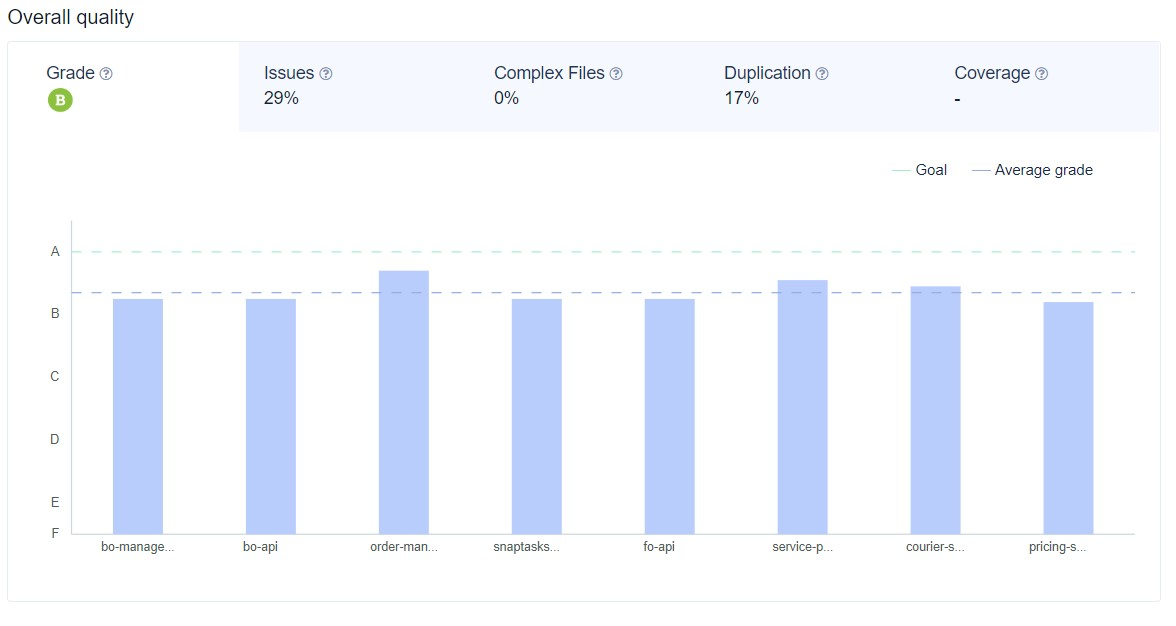
\includegraphics[width=\textwidth,keepaspectratio]{chapters/Implementation/assets/codacy-grade.jpg}
\caption[Codacy grade to SnapTasks projects]{Codacy grade to SnapTasks projects}
\label{fig:codacyGrade}
\end{figure}


\section{User Interfaces}
The user interface is one of the most critical topics for the success of a commercial software project. The user needs to find the application easy to use, attractive and consistent on all pages. The \gls{UI} is mostly important because it can turn visitors into buyers, as it facilitates the interactions between them and the system \parencite{uiDesignImportance}.
\par
The \gls{UI}s are also very important because it combines both the functional requirements of the system (what it will do) and the non-functional requirements (how it will be done), specified in sections \ref{sec:functional-requirements} and \ref{sec:non-functional-requirements}, respectively. The user interfaces can be considered the face of a given feature, since it is what the user will see, when interacting with the system.
\par
In this section, the most important pages of the two end-user applications (SnapTasks Portal, section \ref{sub:UI_SnaptasksPortal}, and SnapTasks BO Management, section \ref{sub:UI_BOManagement}) will be presented, grouped by the application they belong.


\subsection{SnapTasks Portal}
\label{sub:UI_SnaptasksPortal}
The SnapTasks Portal is the front-office application which the final customer will use. It provides features such as place order, check order history and check available services. Since this is the application where the customers will access, it is the one where there is a bigger need for a good \gls{UI}. 

\par

The most important pages of this application are the \textbf{Login Page}, the \textbf{Service Provider Listing Page}, the \textbf{Service Listing Page}, the \textbf{Service Display Page}, the \textbf{Checkout Page} and the \textbf{Order History Page}. These pages are described below.

\clearpage
\subsubsection{Login Page}

The login page is the page where the user will make the authentication, which will then allow him/her to access more actions, such as order history and place orders. The login may be done in two different ways: the first is to use an account that was previously created on the SnapTasks platform, using e-mail and password. the other is to use one external authentication service. Currently, there are two different authentication services: Facebook and Google. The figure \ref{fig:snaptasksLogin} presents the \gls{UI} of the login page.

\begin{figure}[ht]
\centering
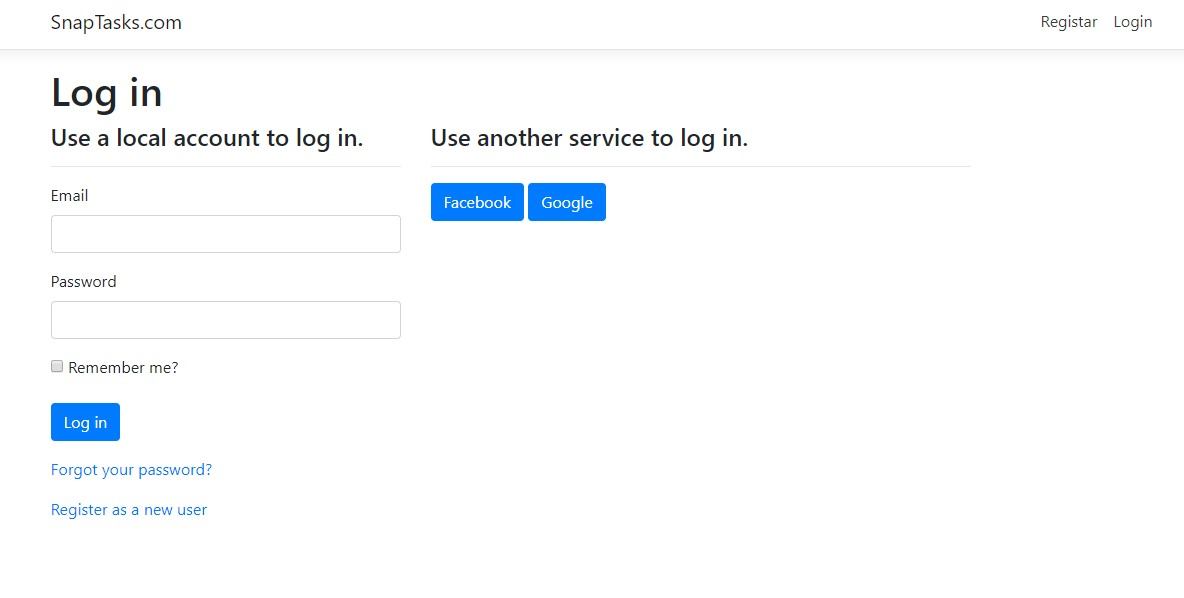
\includegraphics[width=0.65\textwidth,keepaspectratio]{chapters/Implementation/assets/snaptasks-login.jpg}
\caption[SnapTasks login page]{SnapTasks login page}
\label{fig:snaptasksLogin}
\end{figure}


\subsubsection{Service Provider Listing Page (SPLP)}

The \gls{SPLP} is one of the most important pages in the SnapTasks Portal, since it serves as the home page of the application. The main purpose of this page is to present the service providers available on the platform. To that responsibility are added the ones of a home page, which are mainly to catch the attention of the end user and make it appealing to browse the website. The figure \ref{fig:snaptasksSPLP} presents the \gls{GUI} of this page.

\begin{figure}[ht]
\centering
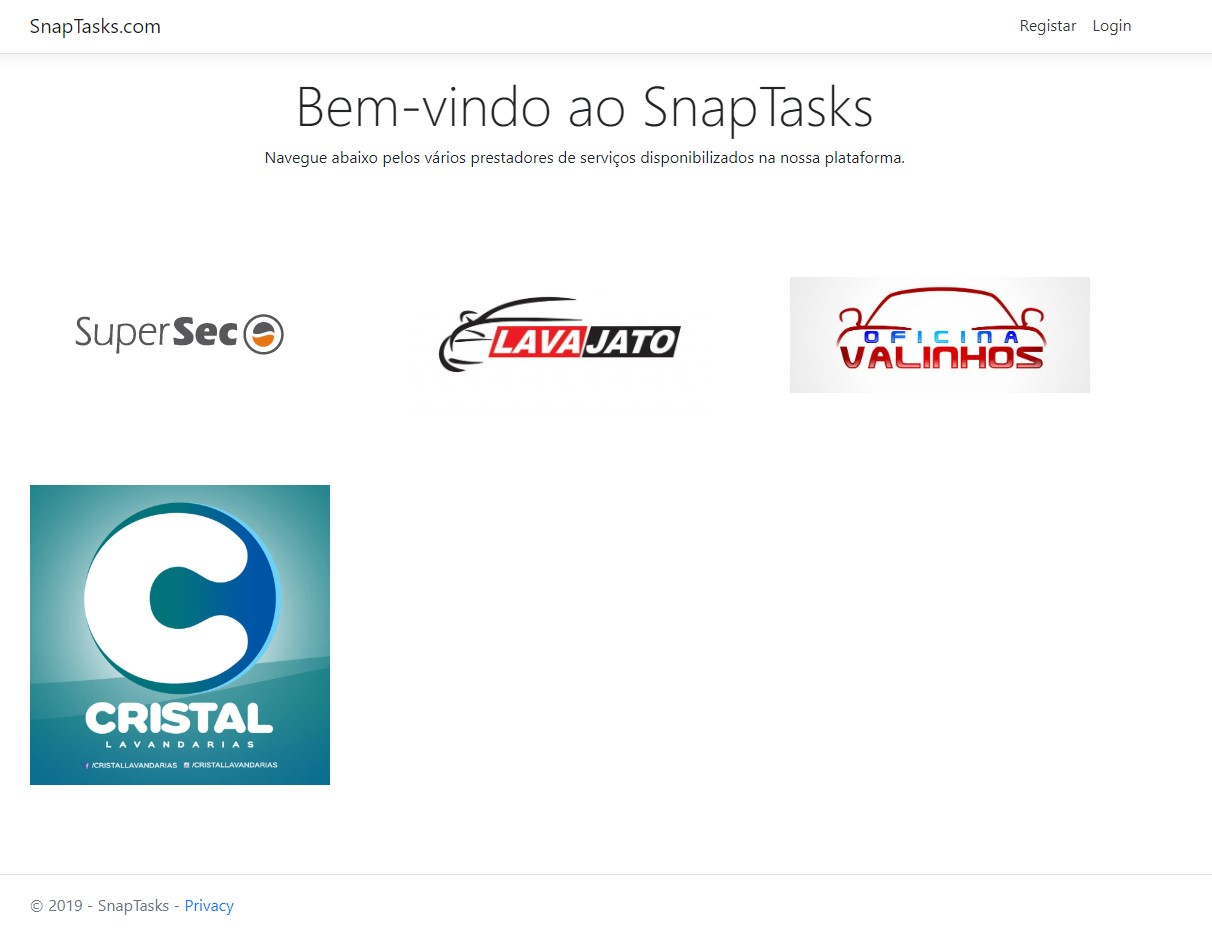
\includegraphics[width=0.65\textwidth,keepaspectratio]{chapters/Implementation/assets/snaptasks-splp.jpg}
\caption[SnapTasks service provider listing page]{SnapTasks service provider listing page}
\label{fig:snaptasksSPLP}
\end{figure}

\clearpage
\subsubsection{Service Listing Page (SLP)}
\label{sub:service-listing-page}
The \gls{SLP} is accessed when the user selects a service provider in the \gls{SPLP}. This page presents the list of services that are provided by the selected \gls{SP}. Besides the name of the service, it also presents a description of the service and its price. The figure \ref{fig:serviceListingPage} presents the \gls{UI} of this page.

\begin{figure}[!ht]
\centering
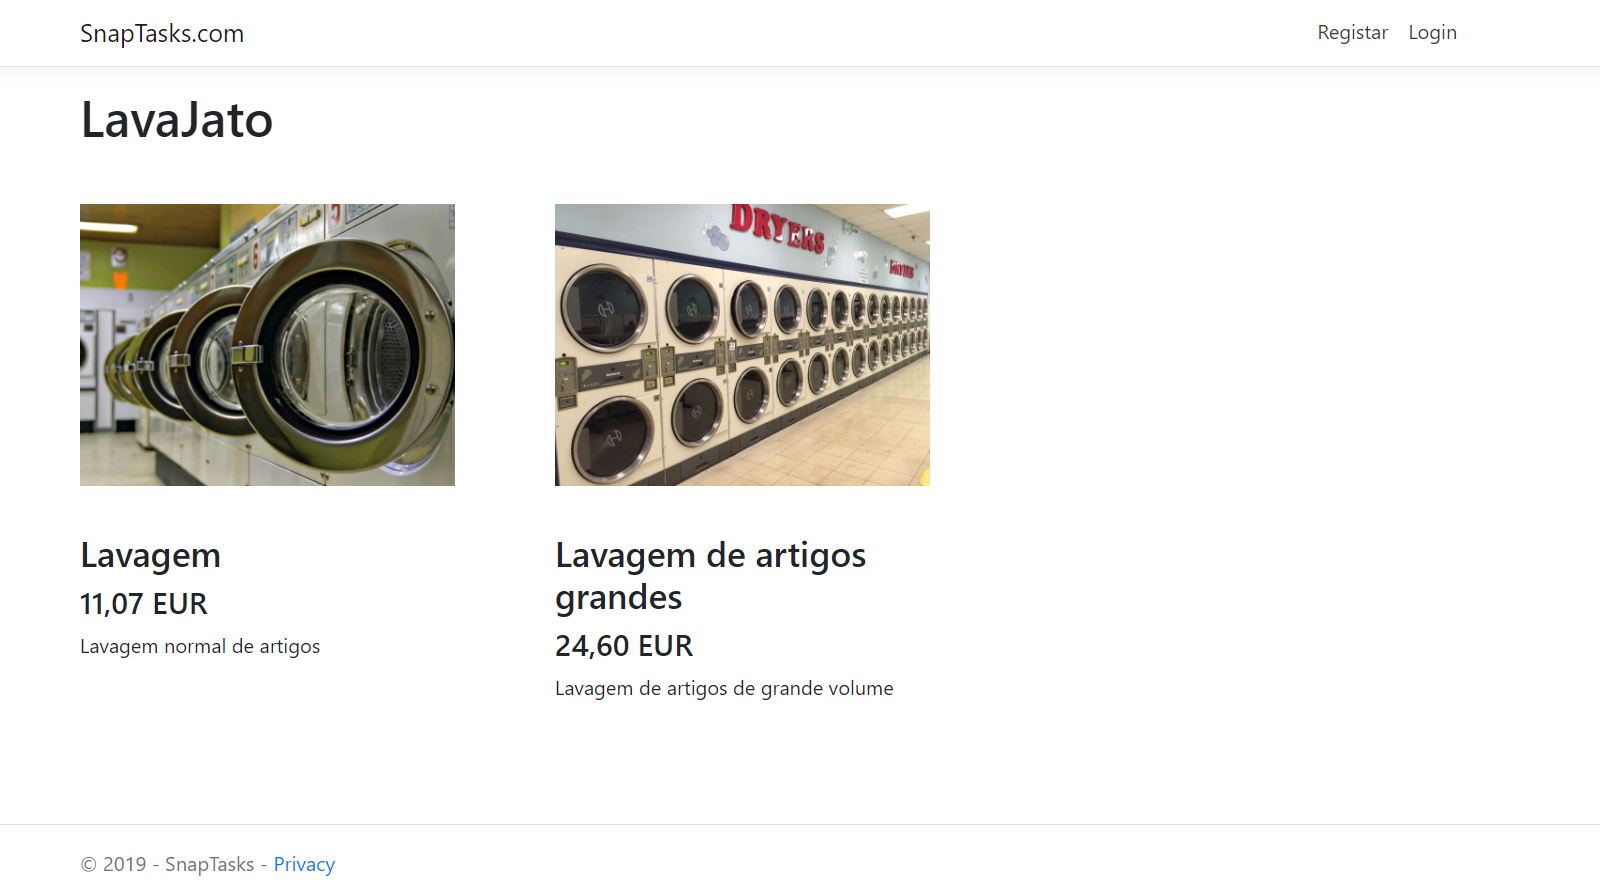
\includegraphics[width=0.9\textwidth,keepaspectratio]{chapters/Implementation/assets/snaptasks-slp.PNG}
\caption[Service Listing Page of a Service Provider]{Service Listing Page of a Service Provider}
\label{fig:serviceListingPage}
\end{figure}


\subsubsection{Service Display Page (SDP)}
When the user selects a service in the \gls{SLP}, he/she is redirected to the \gls{SDP}. This page has as its main purpose to display the details of the selected service. It provides information such as a more detailed description, the base price, the \gls{VAT} and discounts (if any) and the final price. This page also provides the option for the user to place an order for that service. The \gls{UI} of that page is presented in figure \ref{fig:snaptasksSDP}.

\begin{figure}[ht]
\centering
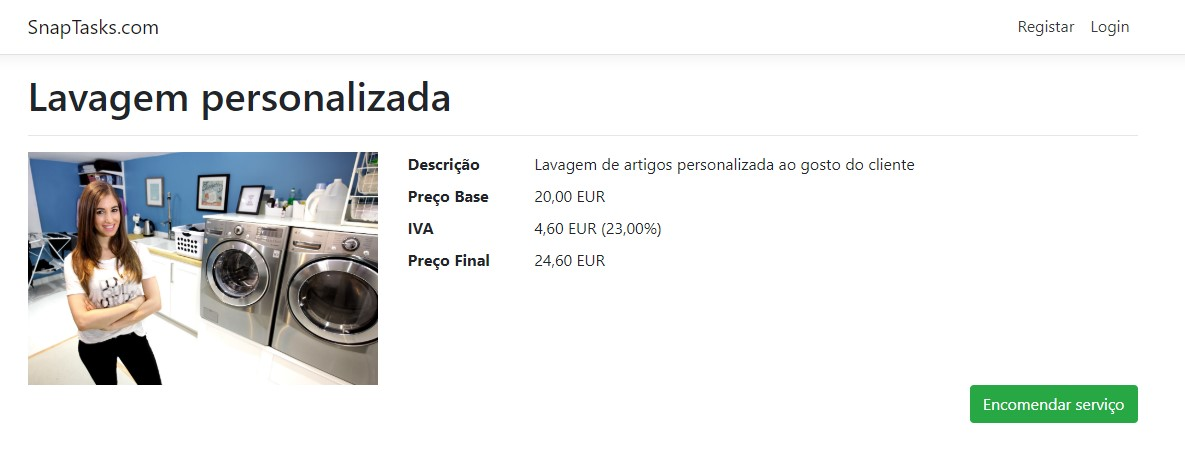
\includegraphics[width=0.9\textwidth,keepaspectratio]{chapters/Implementation/assets/snaptasks-sdp.jpg}
\caption[SnapTasks service display page]{SnapTasks service display page}
\label{fig:snaptasksSDP}
\end{figure}

\clearpage
\subsubsection{Checkout Page}
The checkout page is the page where the customer places an order. It provides the information of the selected service, informs the total value of the order and asks for the information needed to fulfill the order (date of pickup, billing and pickup address and payment information).
\par

For the payment processing, SnapTasks integrates with a third-party payment provider, Stripe, that processes the payments in a secure way. Stripe also provides tools for testing purposes, as several test credit cards.

\par

This page is presented in figure \ref{fig:snaptasksCheckout}.
\begin{figure}[ht]
\centering
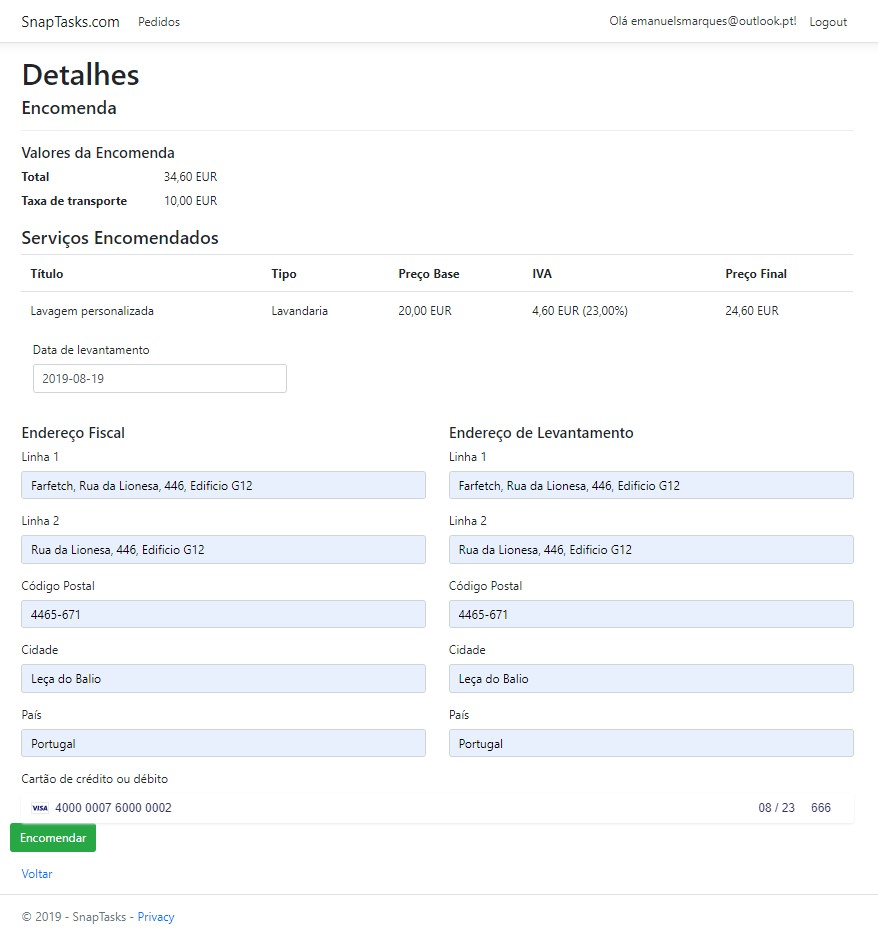
\includegraphics[width=\textwidth,keepaspectratio]{chapters/Implementation/assets/snaptasks-checkout.jpg}
\caption[SnapTasks checkout page]{SnapTasks checkout page}
\label{fig:snaptasksCheckout}
\end{figure}


\subsubsection{Order Details Page}
To access further information regarding an order, the user can open the details, in the order history page. This will redirect the user to the order details page. This page presents all the relevant information that concerns the selected order. The page presents the ordered services, the billing and pickup address, the values of the order (both final price and total. Check how these fields are calculated in section \ref{sec:Implementation_DomainModel}), the order status and the pickup date.

\par

The \gls{UI} of this page is presented in figure \ref{fig:snaptasksOrderDetails}.

\begin{figure}[ht]
\centering
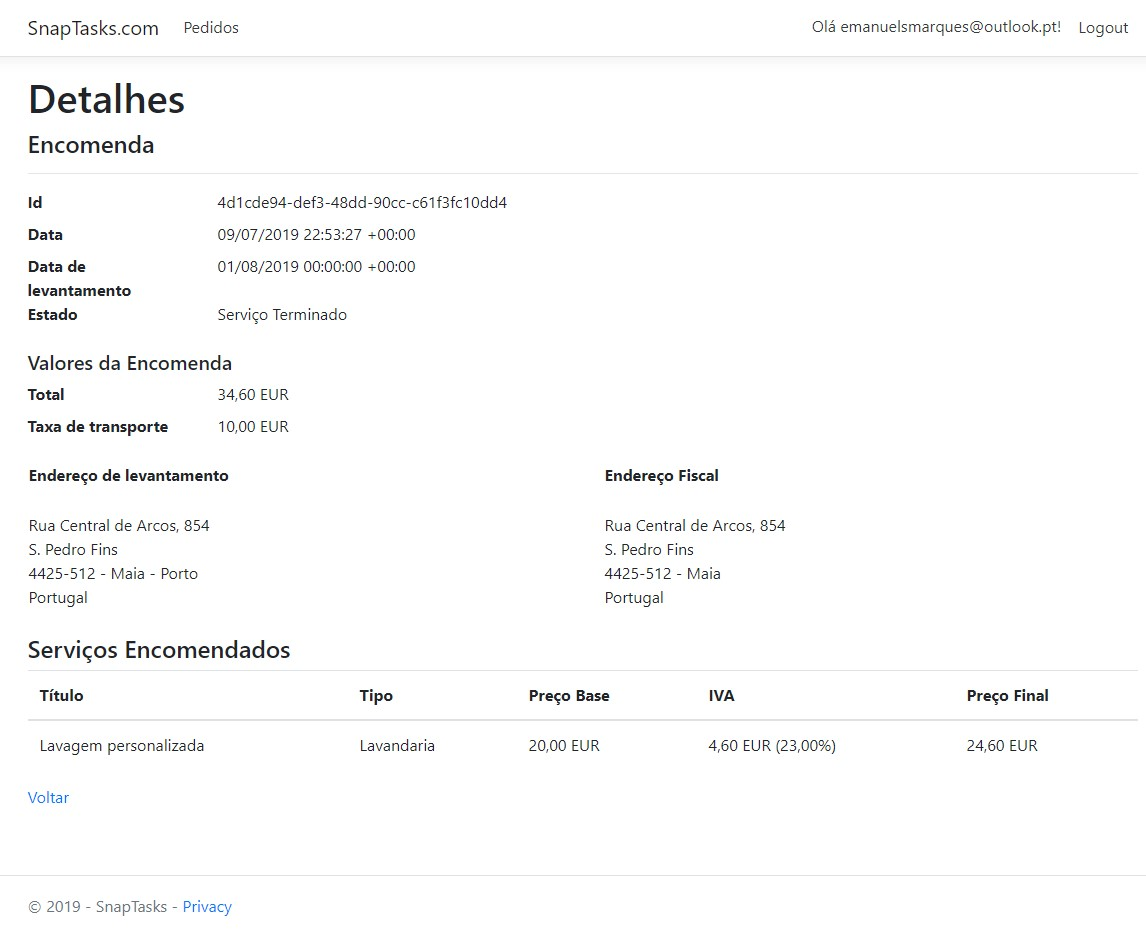
\includegraphics[width=\textwidth,keepaspectratio]{chapters/Implementation/assets/snaptasks-orderDetails.jpg}
\caption[SnapTasks order details page]{SnapTasks order details page}
\label{fig:snaptasksOrderDetails}
\end{figure}


\clearpage
\subsubsection{Order History Page}
The order history presents the customer all the orders he/she had placed in the past. This page shows basic information about the order, such as the identifier, the creation date, the total value and the current status. With this page, it is possible to have an awareness of all the orders that were placed and their status. The figure \ref{fig:snaptasksOrderHistory} presents the \gls{UI} of this page.

\begin{figure}[ht]
\centering
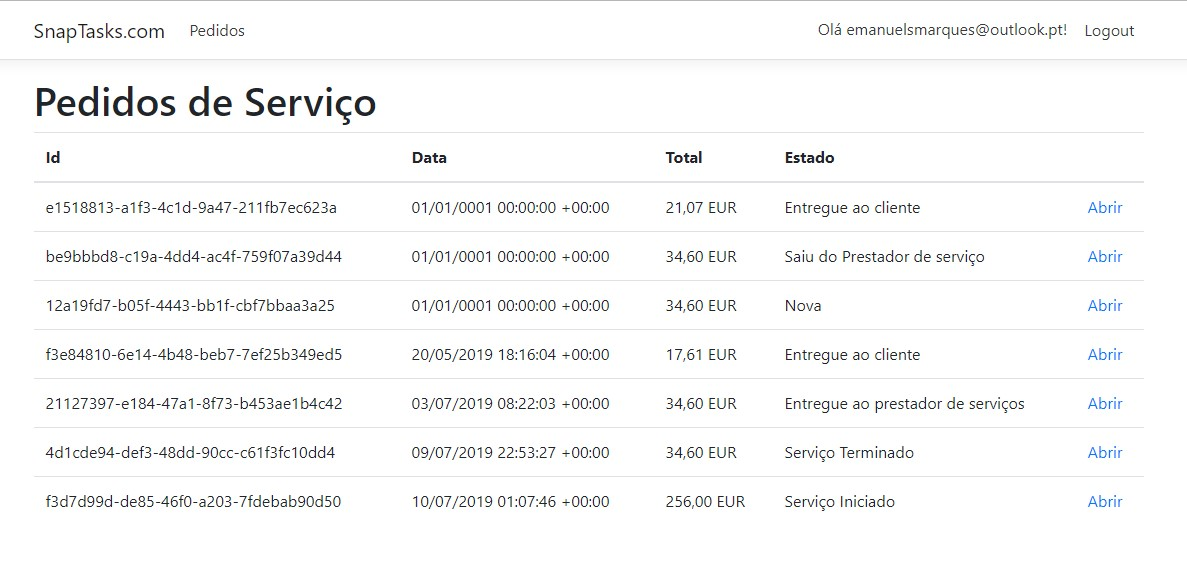
\includegraphics[width=\textwidth,keepaspectratio]{chapters/Implementation/assets/snaptasks-orderhistory.jpg}
\caption[SnapTasks order history page]{SnapTasks order history page}
\label{fig:snaptasksOrderHistory}
\end{figure}

\clearpage

\clearpage
\subsection{SnapTasks Back-Office Management}
\label{sub:UI_BOManagement}
SnapTasks BO Management is an application whose purpose is to provide back-office and management tools. This application is designed to be used mostly by the operations teams who have the responsibility to manage the service providers, the couriers and the orders.
\par
Since this application is not to be used by final customers, the \gls{UI} that is used is not as critical as in the SnapTasks Portal. However, it is still very important that the use of features is intuitive and easy to learn, since the less time something takes to be done, the cheaper it will be.

\par

The pages of this application are grouped into three main categories: 

\begin{itemize}
    \item \textbf{Service Provider Management Pages}, which are the pages where the \gls{SP}s and their services will be listed, created, edited and disabled;
    \item \textbf{Order Management Pages}, where the placed orders can be listed, accessed and processed;
    \item \textbf{Courier Management Pages}, whose pages have the purpose of creation, edit and disable couriers.
\end{itemize}

These pages are further detailed and presented in the next sections.


\subsubsection{Service Provider Management Pages}

The Service Provider Management pages are the group of pages that provide tools to manage the service providers and their services. It is possible to create, disable, and edit both the service providers and its services. For the last case, it is also possible to update the price of a service. These pages can be accessed by the administrators of the platform, who can create and edit any \gls{SP} and its services, and by the service provider's account, who can just edit their information and services. 

\par

The figure \ref{fig:snaptasksSPList} presents the page that lists the current active service providers in the platform and the figure \ref{fig:snaptasksSPDetails} shows the details of a service provider, and which services it provides.

\begin{figure}[!ht]
\centering
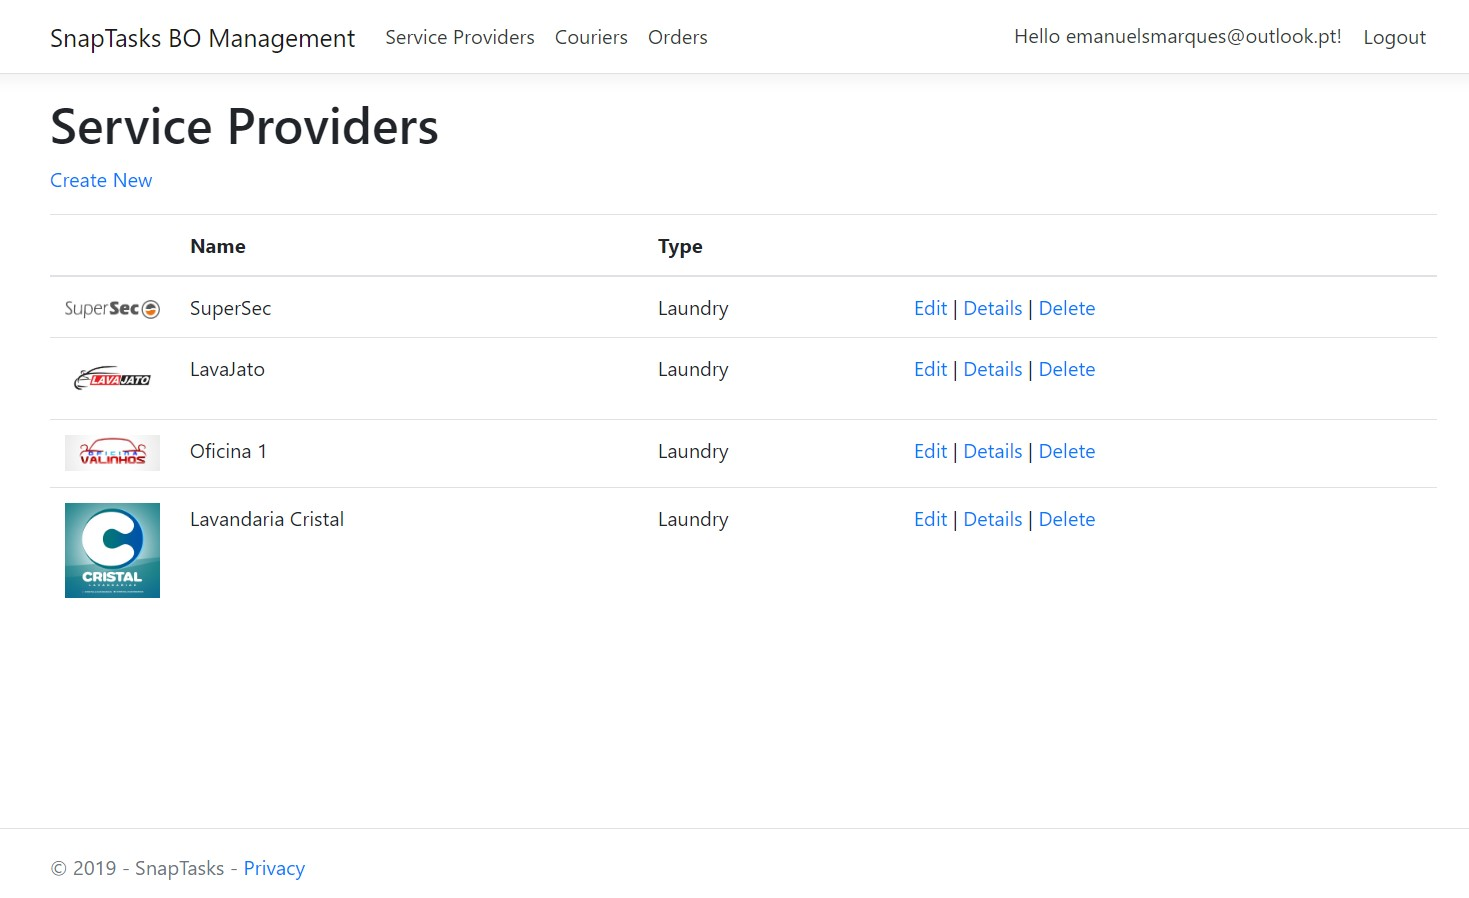
\includegraphics[width=0.7\textwidth,keepaspectratio]{chapters/Implementation/assets/snaptasks-bo-listSP.jpg}
\caption[List of service providers page]{List of service providers page}
\label{fig:snaptasksSPList}
\end{figure}

\begin{figure}[!ht]
\centering
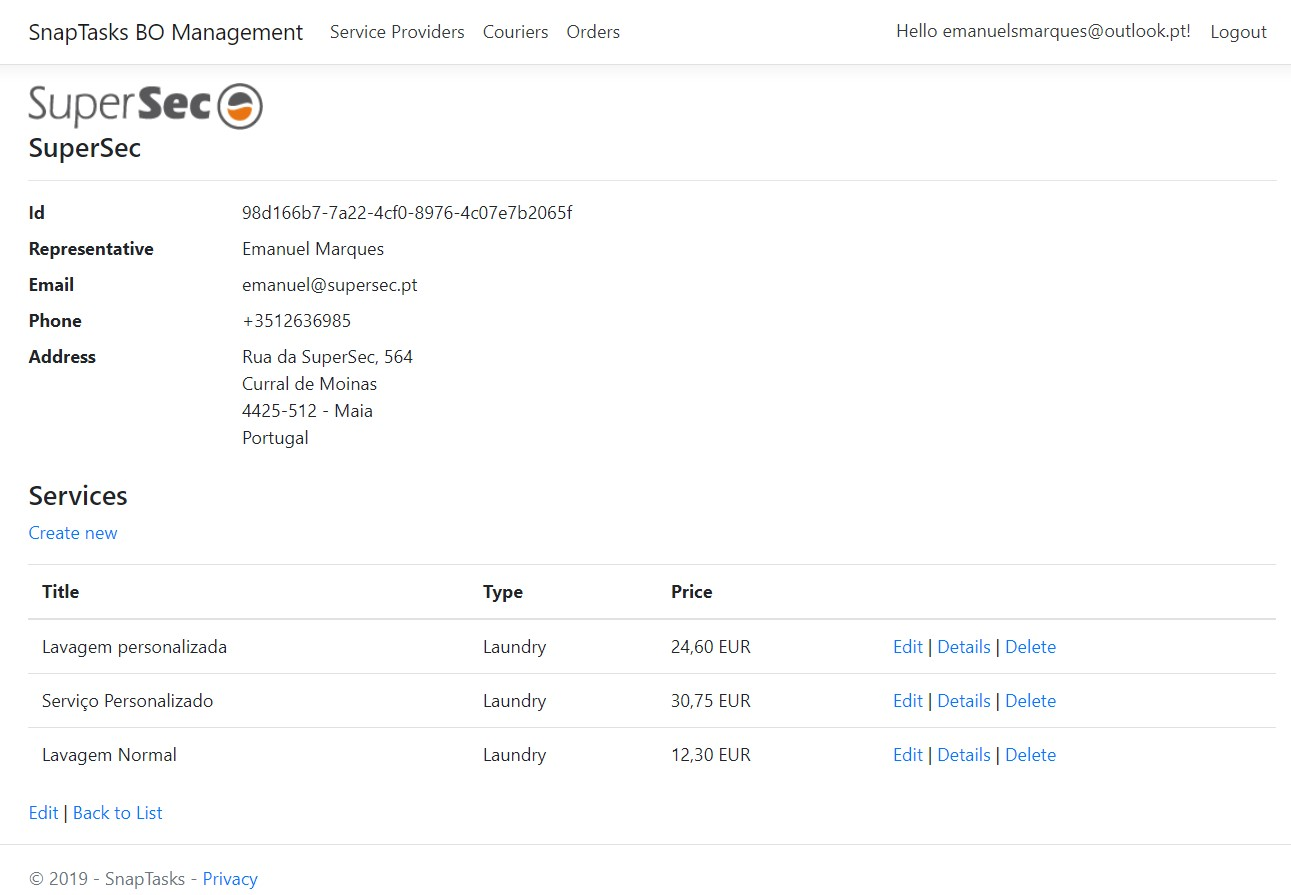
\includegraphics[width=0.8\textwidth,keepaspectratio]{chapters/Implementation/assets/snaptasks-bo-detailsSP.jpg}
\caption[Service Provider details page]{Service Provider details page}
\label{fig:snaptasksSPDetails}
\end{figure}


\subsubsection{Courier Management Pages}
Similarly to the previous pages, this group contains the features to create, edit and disable couriers. This is essentially an administration feature since only platform administrators have access to it.
\par
The figure \ref{fig:snaptasksCourierList} presents the page that lists all the available couriers.

\begin{figure}[ht]
\centering
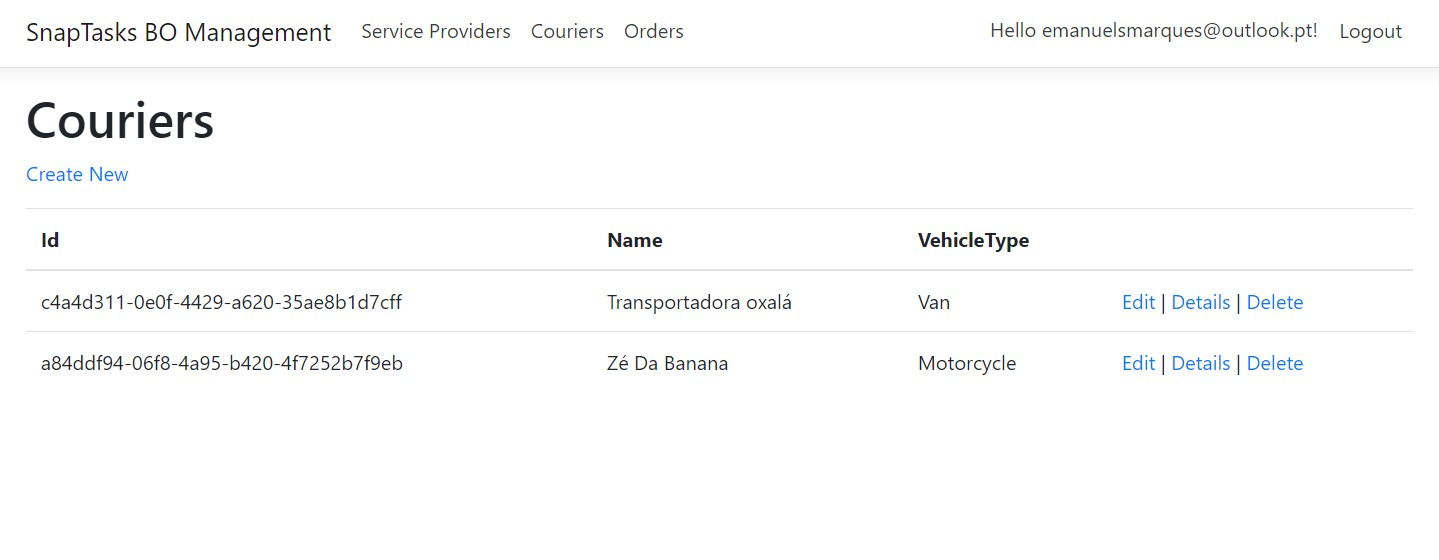
\includegraphics[width=\textwidth,keepaspectratio]{chapters/Implementation/assets/snaptasks-bo-listCouriers.jpg}
\caption[Courier list page]{Courier list page}
\label{fig:snaptasksCourierList}
\end{figure}


\subsubsection{Order Management Pages}

The order management pages are the pages where order information will be available and order processing features (like changing step, or courier assignment) will be available. Here is also possible to view the details of a given order and check the order history.

\par

The figure \ref{fig:snaptasksOrderList} presents the page that lists the placed orders to be processed in the platform and the ones that were already processed. The figure \ref{fig:snaptasksOrderDetailsBO} shows the details of a given order.

\begin{figure}[!ht]
\centering
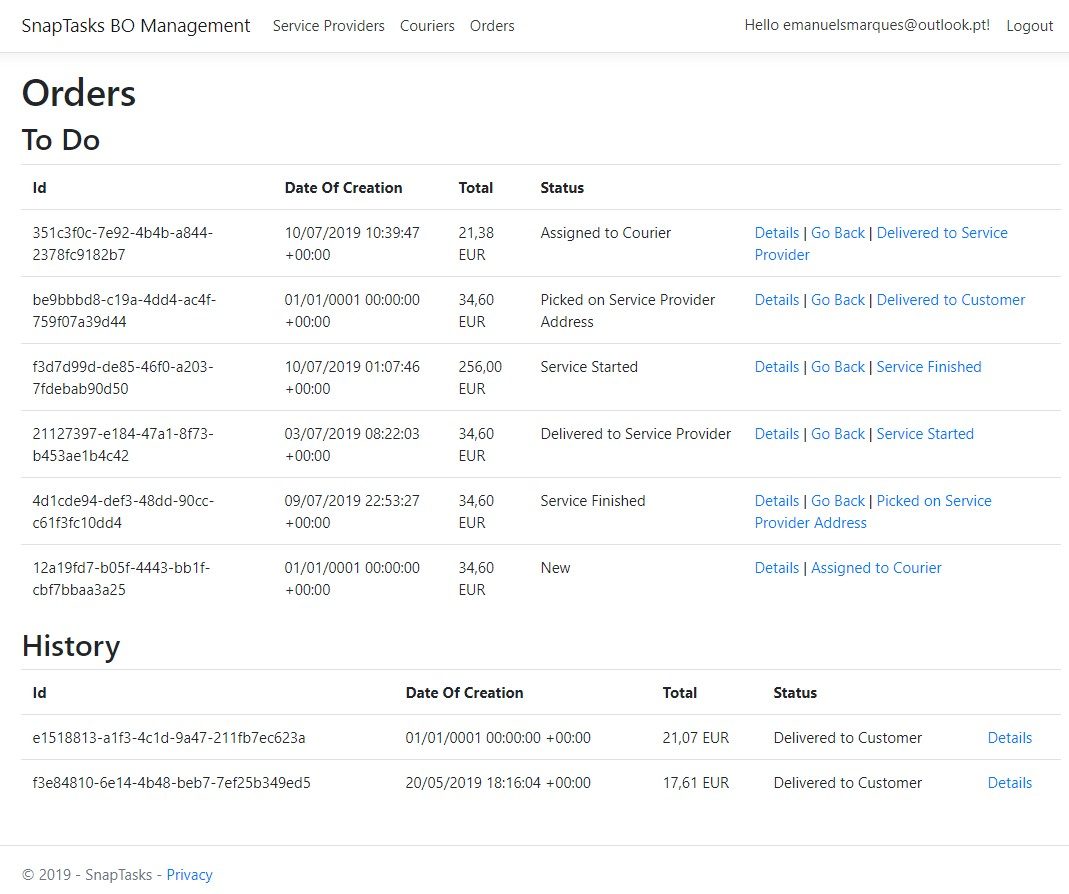
\includegraphics[width=0.8\textwidth,keepaspectratio]{chapters/Implementation/assets/snaptasks-bo-todo.jpg}
\caption[Order Processing Page]{Order Processing Page}
\label{fig:snaptasksOrderList}
\end{figure}

\begin{figure}[!ht]
\centering
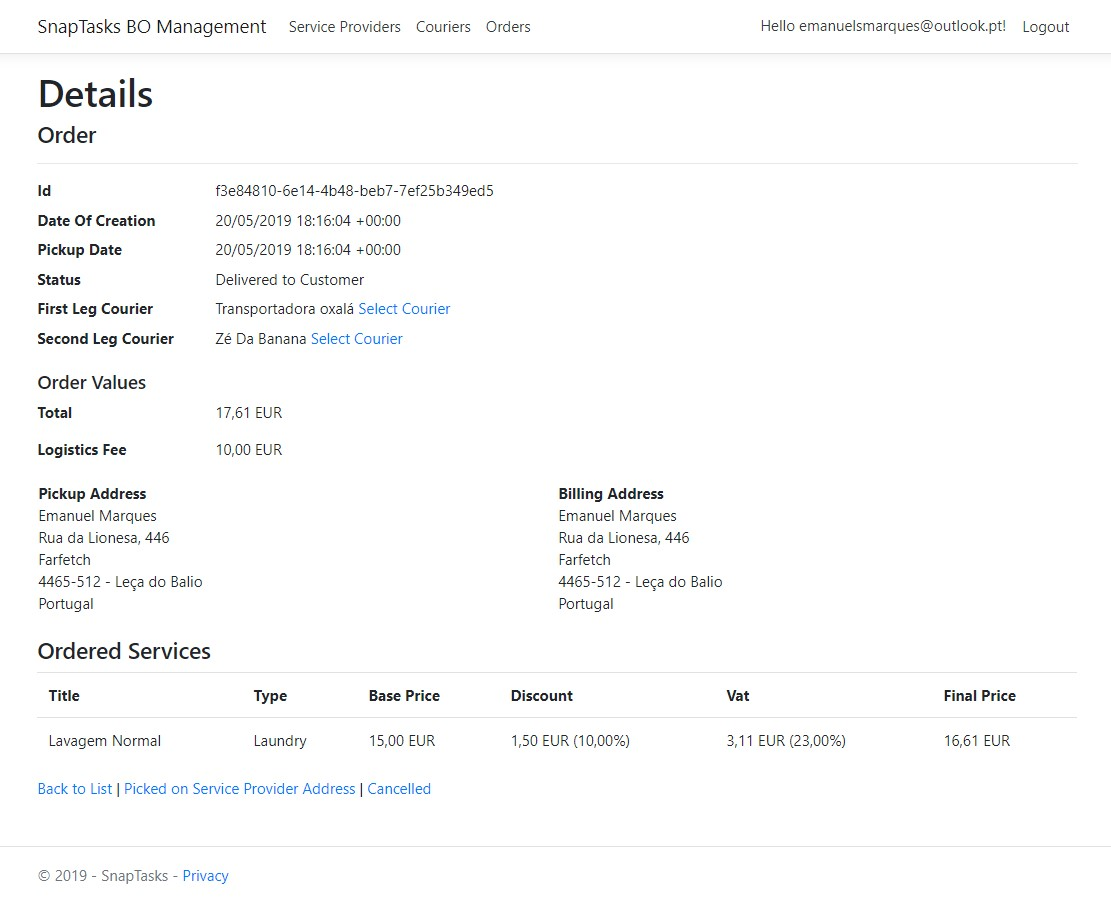
\includegraphics[width=0.8\textwidth,keepaspectratio]{chapters/Implementation/assets/snaptasks-bo-orderDetails.jpg}
\caption[Order details page]{Order details page}
\label{fig:snaptasksOrderDetailsBO}
\end{figure}



\chapter{Evaluation of the Solution} % Main chapter title
\label{chap:solution_evaluation} 
After developing a new solution or project it is necessary to review if the final product has met the initial expectations. To accomplish this, the solution needs to be evaluated using a methodology that defines the system's functional and non-functional requirements. The designed model represents the ideal solution. The system is evaluated in several aspects of the dimensions, taking into account if the requirement was or not fulfilled, and with what quality.
\par
In this chapter, it will be presented the methodology that was used and how it was used.

\section{Evaluation Methodology}
\label{sec:evaluation_methodology}
To evaluate the quality of the solution, it was chosen to apply a \gls{QEF}. \gls{QEF} is used to identify the relevant quality factors to a certain business and to help on the definition of the metrics to objectively measure the quality factors that were identified \parencite{qef}. A model (available on appendix \ref{AppendixB}) was made to represent the ideal system. This model is divided into three different dimensions:  
\begin{itemize}
    \item Functional
    \item Security
    \item Efficiency
\end{itemize}

\par
The functional dimension is divided into two factors: the functional requirements and the user interaction. The first lists all needed use cases to be accomplished for the project to be a success. These will be measured by either the user has access to the functionality or not. In the case of FF11 and FF12, an intermediate point is acceptable, where it is available for just some of the actors. The second factor refers to the usability of the application. This will be measured mostly by questioning the users for their experience.
\par
The second dimension, security, refers to the concerns relatively to, as the name suggests, security of the platform. In this case, the only concerns that exist are associated to the security it, therefore it is its only factor. Similarly to the previous dimension, it will be measured by having or not fulfilled each of the requirements. There are intermediate positions for RN01 and RN02 when they are not put into practice every time.
\par
Lastly, the third dimension that will be evaluated is the efficiency. This dimension was split into two factors. The first concerns the overall structure of the page and the user can access its contents in an intuitive and direct way. The second one relates to the navigation resilience. In this factor, the requirements regarding the error handling and progress bars, showing progress for long tasks, will be evaluated. Both the factors of this dimension will be measured by having or not fulfilled the requirement. The only exception is the requirement EN02, where it is acceptable to have up to two long tasks not showing a progress bar.
\par
For this project to be successful, the quality factor in the \gls{QEF} should be above 90\% and have no dimension with a quality below 80\%. 


\section{Evaluation Results}
The model presented in section \ref{sec:evaluation_methodology} was applied to the final version of the prototype developed in the scope of this thesis. This version was finished in August \nth{6}, 2019 and the evaluation was made in September \nth{2}, 2019. 
\par
The requirements of the dimensions were weighted taking into account the priority and importance for the correct functioning of the platform, being 10 the most important and 2 the least important.
\par
The \textbf{functional dimension} is the biggest dimension since it contains all the use cases required by the platform. At this dimension there were three requirements that were postponed to a second version of the platform:

\begin{itemize}
    \item FF02 - Apply as a Service Provider
    \item FF03 - Apply as a Courier
    \item FF09 - Evaluate Experience
\end{itemize}

These requirements lost priority in comparison to others because in a first delivery, the prototype will run with a test service provider and limited number of couriers. The same happens for the FF09, where in a first phase, the experience will be reported directly to the existing service provider.
\par
This dimension was concluded with an estimated evaluation of 95.64\%.

\par

The second dimension, \textbf{security}, is one of the most important aspects in an e-commerce platform. It may attract or withdraw attention from possible customers and directly affects the reliability of the website. This dimension was completed in 100\%.

\par

Lastly, there is the \textbf{efficiency dimension}, which includes both the structure and navigation resilience. Since the platform still lacks beta testing in a real scenario (having real customers, couriers and service providers), there still room for improvement here. For this reason, the requirement \textit{EN03 - Application runtime does not have errors, and unexpected errors should be well treated} was only partially accomplished. With this, the evaluation result of this dimension was 83.33\%.

\par

Looking at the solution as a whole, the system had an evaluation of 95\%. This is a result that was better than expected. In the beginning of the project, the objective was to have a evaluation of at least 90\%. The system attained 5\% above than the required. It was also required to have no dimension with its evaluation below 80\%. As it was previously explained, the lowest score was 83\%.
\par
In the last page of the appendix \ref{AppendixB}, it is possible to check the evaluation matrix.

\section{Usability Surveys}
To understand how the platform meets the users needs, two surveys were run: one for the final customer perspective, and other for the service provider perspective. In the next sections, both surveys will be analyzed. 

\subsection{Customer Perspective Survey}
The first survey has as its purpose understand how the final customer feels about the usability of the SnapTasks portal. It includes a tutorial to place an order and explains how to use some of the  main features. In the appendix \ref{AppendixD} it is possible to check the original inquiry, and in the appendix \ref{AppendixF}, it is possible to consult the summary of the answers. This inquiry was made to seven people of different backgrounds.

\subsubsection{How do you rate the ease of registration and log in?}
This question has as its main purpose the evaluation of the log in and registration process. 
\par 
This question asks the user to evaluate in a scale of 1 to 5, where 1 is \textit{Very Hard} and 5 is \textit{Very Easy}. 
\par
This question had a result of \textbf{5}, out of 5. 


\subsubsection{How do you rate the presentation of service providers?}
This question has as its main purpose the evaluation of the home page, which is also the \gls{SPLP}. 
\par 
This question asks the user to evaluate in a scale of 1 to 5, where 1 is \textit{Very Hard to Understand} and 5 is \textit{Very Easy to Understand}. 
\par
This question had a result of \textbf{4.57}, out of 5. 

\subsubsection{How do you rate a service provider's presentation of services?}

This question has as its main purpose the evaluation of the \gls{SLP} of a given service provider and how those services are presented to the user. 
\par 
This question asks the user to evaluate in a scale of 1 to 5, where 1 is \textit{Very Hard to Understand} and 5 is \textit{Very Easy to Understand}. 
\par
This question had a result of \textbf{4.43}, out of 5. 

\subsubsection{Regarding the detail given on the page of a service, was the information sufficient?}

This question has as its main purpose the evaluation of the \gls{SDP} of a given service and how the details of a service are presented to the user. 
\par
This question asks the user to evaluate in a scale of 1 to 5, where 1 is \textit{Very Insufficient} and 5 is \textit{More than Sufficient}. 
\par
This question had a result of \textbf{4}, out of 5. 

\subsubsection{Was the price of a given service clear to you?}

This question has as its main purpose the evaluation of how clear the price of a given service was to the user.
\par
This question asks the user to evaluate in a scale of 1 to 5, where 1 is \textit{Not clear at all} and 5 is \textit{Very clear}. 
\par
This question had a result of \textbf{4.71}, out of 5. 

\subsubsection{How do you rate the ease of placing an order?}

This question has as its main purpose the evaluation the order placing and checkout experience. 
\par
This question asks the user to evaluate in a scale of 1 to 5, where 1 is \textit{Very hard} and 5 is \textit{Very easy}. 
\par
This question had a result of \textbf{4.86}, out of 5. 

\subsubsection{Was the data presented about the order placed (after purchase) clear?}

This question has as its main purpose the evaluation the order details page. 
\par 
This question asks the user to evaluate in a scale of 1 to 5, where 1 is \textit{Not clear at all} and 5 is \textit{Very clear}. 
\par
This question had a result of \textbf{4.86}, out of 5.

\subsubsection{How do you rate the information given in the order history?}

This question has as its main purpose the evaluation of the order history page and how the order history is presented to the user. 
\par
This question asks the user to evaluate in a scale of 1 to 5, where 1 is \textit{Very Insufficient} and 5 is \textit{More than Sufficient}. 
\par
This question had a result of \textbf{4.29}, out of 5. 

\subsubsection{Summary}
In this survey, the results of all questions were above 4, which is an excellent result. The graph in the figure \ref{fig:CustomerSurveyResults} presents a summary of the acquired results.


\begin{figure}[ht]
\centering
 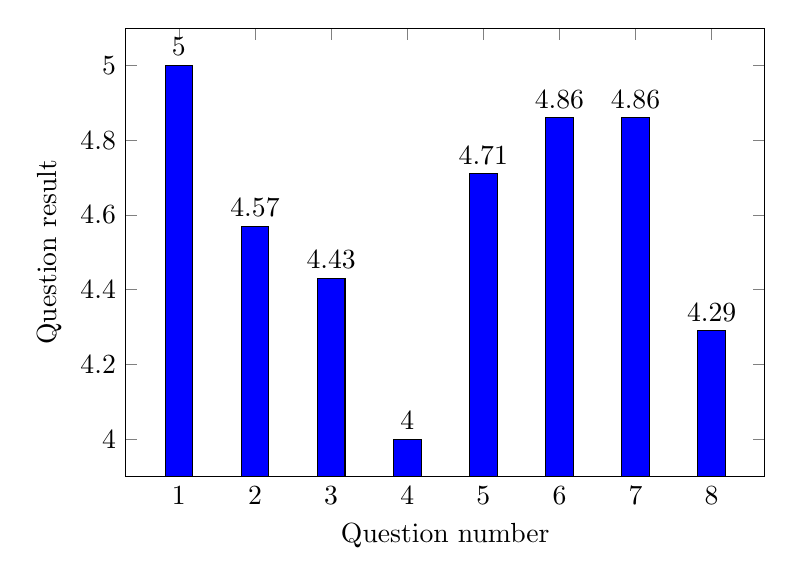
\begin{tikzpicture}
        \begin{axis}[
            symbolic x coords={1, 2, 3, 4, 5, 6, 7, 8},
            ylabel=Question result,
            xlabel=Question number,
            width=0.8\textwidth,
            height=0.6\textwidth,
            nodes near coords,
            nodes near coords align={vertical},
          ]
            \addplot[ybar,fill=blue] coordinates {
                (1,  5)
                (2,  4.57)
                (3,  4.43)
                (4,  4)
                (5,  4.71)
                (6,  4.86)
                (7,  4.86)
                (8,  4.29)
            };
        \end{axis}
    \end{tikzpicture}
\caption{Summary of results of the Customer Perspective Survey}
\label{fig:CustomerSurveyResults}
\end{figure}


\subsection{Service Provider Perspective Survey}
The second survey has as its purpose understand how service provider feels about the usability of the SnapTasks BackOffice Management app. It includes a tutorial of how to use some of the  main features. In the appendix \ref{AppendixE} it is possible to check the original inquiry, and in the appendix \ref{AppendixG}, it is possible to consult the summary of the answers. This inquiry was made to five people that work in service provision business.

\subsubsection{How do you rate the ease of log in?}
This question has as its main purpose the evaluation of the log in process. 
\par 
This question asks the user to evaluate in a scale of 1 to 5, where 1 is \textit{Very Hard} and 5 is \textit{Very Easy}. 
\par
This question had a result of \textbf{4.4}, out of 5. 

\subsubsection{How do you rate the presentation of service providers?}
This question has as its main purpose the evaluation of the presentation of the several service providers.
\par 
This question asks the user to evaluate in a scale of 1 to 5, where 1 is \textit{Very hard to understand} and 5 is \textit{Very easy to understand}. 
\par
This question had a result of \textbf{4}, out of 5. 

\subsubsection{How do you rate a service provider's presentation of services?}

This question has as its main purpose the evaluation of the presentation of the services of a given service provider.
\par 
This question asks the user to evaluate in a scale of 1 to 5, where 1 is \textit{Very hard to understand} and 5 is \textit{Very easy to understand}. 
\par
This question had a result of \textbf{4}, out of 5. 

\subsubsection{Regarding the detail given on the page of a service provider, was the information sufficient?}

This question has as its main purpose the evaluation of the presentation of the information regarding a given service provider. This information includes name, address, representatives and services.
\par 
This question asks the user to evaluate in a scale of 1 to 5, where 1 is \textit{Very insufficient} and 5 is \textit{More than sufficient}. 
\par
This question had a result of \textbf{3.6}, out of 5. 

\subsubsection{How do you rate the ease of updating the price of a service?}

This question has as its main purpose the evaluation of the process of price update on a given service.
\par 
This question asks the user to evaluate in a scale of 1 to 5, where 1 is \textit{Very insufficient} and 5 is \textit{More than sufficient}. 
\par
This question had a result of \textbf{3.2}, out of 5. 

\subsubsection{Was the presentation of the service data clear?}

This question has as its main purpose the evaluation of the presentation of details of a given service.
\par 
This question asks the user to evaluate in a scale of 1 to 5, where 1 is \textit{Not clear at all} and 5 is \textit{Very clear}. 
\par
This question had a result of \textbf{4}, out of 5. 

\subsubsection{Was the price presentation clear?}

This question has as its main purpose the evaluation of how clear the price presentation was to the user.
\par 
This question asks the user to evaluate in a scale of 1 to 5, where 1 is \textit{Not clear at all} and 5 is \textit{Very clear}. 
\par
This question had a result of \textbf{4.2}, out of 5.

\subsubsection{How do you rate the information given in the order history?}

This question has as its main purpose the evaluation of how clear the information present in the order history was.
\par 
This question asks the user to evaluate in a scale of 1 to 5, where 1 is \textit{Not clear at all} and 5 is \textit{Very clear}. 
\par
This question had a result of \textbf{4}, out of 5.

\subsubsection{How do you rate the information given in the details of an order (click "Details")?}

This question has as its main purpose the evaluation of how clear the information present in the order details was.
\par 
This question asks the user to evaluate in a scale of 1 to 5, where 1 is \textit{Not clear at all} and 5 is \textit{Very clear}. 
\par
This question had a result of \textbf{4}, out of 5.

\subsubsection{How do you rate the ease of changing an order status?}

This question has as its main purpose the evaluation of how easy it was to change the order status.
\par 
This question asks the user to evaluate in a scale of 1 to 5, where 1 is \textit{Very hard} and 5 is \textit{Very easy}. 
\par
This question had a result of \textbf{3.6}, out of 5.

\subsubsection{Summary}
In this survey, the results of all questions were above 3, which is an good result, despite being lower than the customer result. The graph in the figure \ref{fig:CustomerSurveyResults} presents a summary of the acquired results.


\begin{figure}[!ht]
\centering
 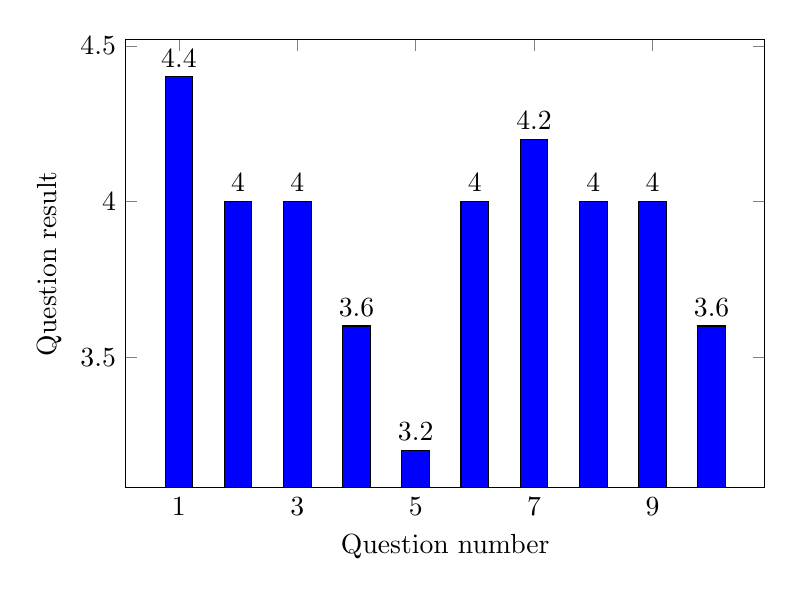
\begin{tikzpicture}
        \begin{axis}[
            symbolic x coords={1, 2, 3, 4, 5, 6, 7, 8, 9, 10},
            ylabel=Question result,
            xlabel=Question number,
            width=0.8\textwidth,
            height=0.6\textwidth,
            nodes near coords,
            nodes near coords align={vertical},
          ]
            \addplot[ybar,fill=blue] coordinates {
                (1,  4.4)
                (2,  4)
                (3,  4)
                (4,  3.6)
                (5,  3.2)
                (6,  4)
                (7,  4.2)
                (8,  4)
                (9,  4)
                (10, 3.6)
            };
        \end{axis}
    \end{tikzpicture}
\caption{Summary of results of the Customer Perspective Survey}
\label{fig:ServiceProviderSurveyResults}
\end{figure}
\pagebreak
\subsection{Results}
The results of both inquiries help us understand the points that should be improved in the future. There is room for improvement specially in the SnapTasks BackOffice Management app. Nevertheless, the results of both surveys were good, since all results were above 3 and taking into account that we are analysing the \gls{MVP} of the platform.
\par
In the SnapTasks portal (Customer Perspective Survey), the results were even better, having all results above 4, proving that the customers are already used to these type of platforms and could easily start using them for service provision.



\chapter{Conclusion} % Main chapter title
\label{chap:Conclusion}
In the final chapter of this dissertation, it is made a critical balance of the project as a whole. The objectives that were successfully fulfilled, the ones that were carried over a second version, the results and future work. The chapter is divided into two sections. The first is focused in approaching the achievements and results of the project. It will be discussed the implemented requirements, the attained objectives and the overall results. In the second section, it is presented the points that passed to a second version of the platform, an overview of possible improvements and enhancements for the growth of the platform. These recommendations aim to make the platform robust and maintainable enough to be a production level product.

\section{Achievements and Results}
The main objective of this thesis was to create a solution to the existent need of a platform that supports e-commerce applied to services where there is a logistical operation for it to be fulfilled. There were several requirements in terms of functionalities and technological challenges which aimed for the solution to be maintainable, dynamic and that supported multiple service providers if needed. The research made showed that there are similar problems that that already have an implemented solution (Uber Eats) and the analysis of its operational implementation helped to understand how our problem could be solved.

\par
To solve the problem, a prototype was developed that responds to the needs that were described in the chapter \ref{sec:chap1_problem_statement}. It provides the main functionalities needed to have the platform running, like allowing the management of service providers and their services, the management o couriers and the possibility to place and process an order in an easy and intuitive way. The developed solution uses a micro-services architecture allowing its growth in the future and facilitating the development by different people/teams. The APIs have a \textit{Swagger} page where it is possible to check its endpoints, the arguments, the response body, the error codes and to make a direct request to the \gls{API}. 
\par
The biggest challenge in the design of the platform was to design the best architecture for the platform. It was needed to decide which services made sense to use and which made not. The outcome was an architecture with two web applications, two \gls{API}s, four services, each one with its own database, all of the communicating seamlessly. Furthermore, the usage of an external payments provider also proved to be a challenge, since each third-party provider has its own rules that one needs to follow in order to integrate with it.

\par
In terms of quality, the platform was evaluated in two different ways. The first one was applying the \gls{QEF} model to the final version. This evaluation had a result of 95\% which is 5\% above the objective that was initially stated. These results proved that the requirements of the project were completed almost entirely. The second evaluation was to use \textit{Codacy} to verify the code quality of the platform components. This evaluation also met the objectives, reaching the B grade from a scale F-A, being A the best grade, and F the worst. To get this grade it was needed a big attention to detail in terms of code quality. 
\par 
The results of the surveys made to possible final customers and service providers also proved the viability of this platform. The first one proved that customers are used to how e-commerce platforms work and are willing to use an e-commerce platform for service provision. The second one, highlighted some improvements that are to be done in the back-office app, but, nevertheless, also had very positive results, proving that this kind of solution can be used for service provision management.
\par
Lastly, there is still some limitations before using the platform in production. It should go through a beta testing phase where real service providers, with real services and real couriers were added to the platform. This will almost certainly raise issues that were not thought during the development of the project. One can say that no application/feature is really tested until it reaches the production environment, since it is very common to find things that were not discussed before.

\section{Future Work}

In the movie \textit{The Social Network}, where the development of Facebook is depicted, it is said that \textit{"a software product is never finished. The way fashion is never finished"}(adapted). Despite being a movie, the sentence is very much real. No software product is ever finished since there is always something to improve. And even if there is not, as the world changes, our code also needs to change.
\par
This platform is no exception to this rule. There is still room for improvements in the existent features. There are still three features that were not developed in the first version. The user interfaces should also be a target of improvements both visually, where they could be redesigned to provide a unique interface that characterizes the brand, and in terms of usability, where \gls{UX} studies should be done to understand what is the best layout for the users of the platform
\par
The platform could also make use of a messaging service, specially for changes that happen to the order. The notification of customers about the progress of their orders, of service providers when there are new orders and couriers about orders ready for pickup are examples of use cases where these technologies could fit very easily.
\par
The platform could also use a system of ticketing for issues that may happen, therefore creating a customer service team that aimed to help the customers for problems they may have.
\par
Lastly, the platform could also integrate with billing software to facilitate the service providers' billing and tax calculations.

%----------------------------------------------------------------------------------------
%	BIBLIOGRAPHY
%----------------------------------------------------------------------------------------

\printbibliography[heading=bibintoc]

%----------------------------------------------------------------------------------------
%	THESIS CONTENT - APPENDICES
%----------------------------------------------------------------------------------------

\appendix % Cue to tell LaTeX that the following "chapters" are Appendices

% Include the appendices of the thesis as separate files from the Appendices folder
% Uncomment the lines as you write the Appendices

% Appendix A

\chapter{Thesis Formalization} % Main appendix title

\label{AppendixA} % For referencing this appendix elsewhere, use \ref{AppendixA}

 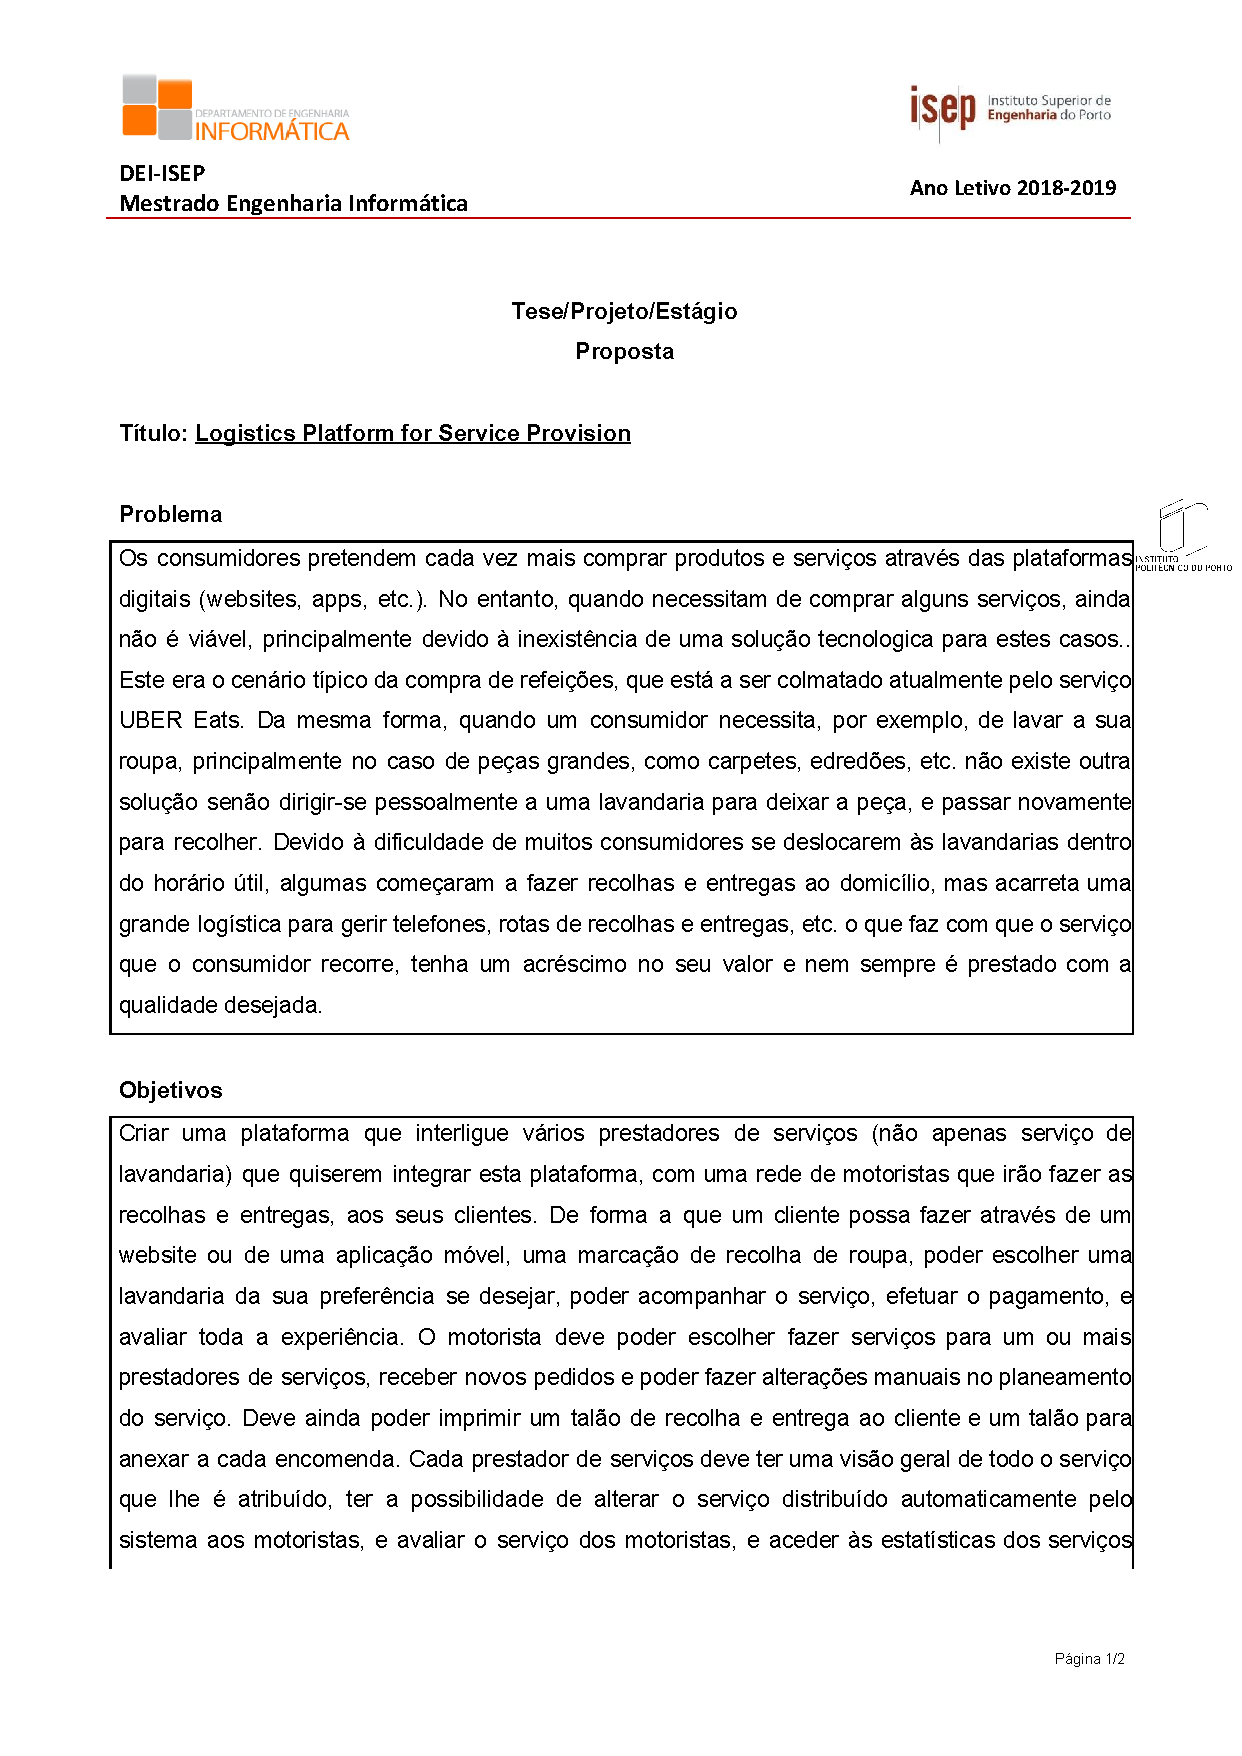
\includegraphics[page=1, width=\textwidth ]{appendices/files/thesis_formal.pdf}

\pagebreak

 \includegraphics[page=2, width=\textwidth ]{appendices/files/thesis_formal.pdf}

\chapter{QEF Solution Evaluation} % Main appendix title

\label{AppendixB} 

 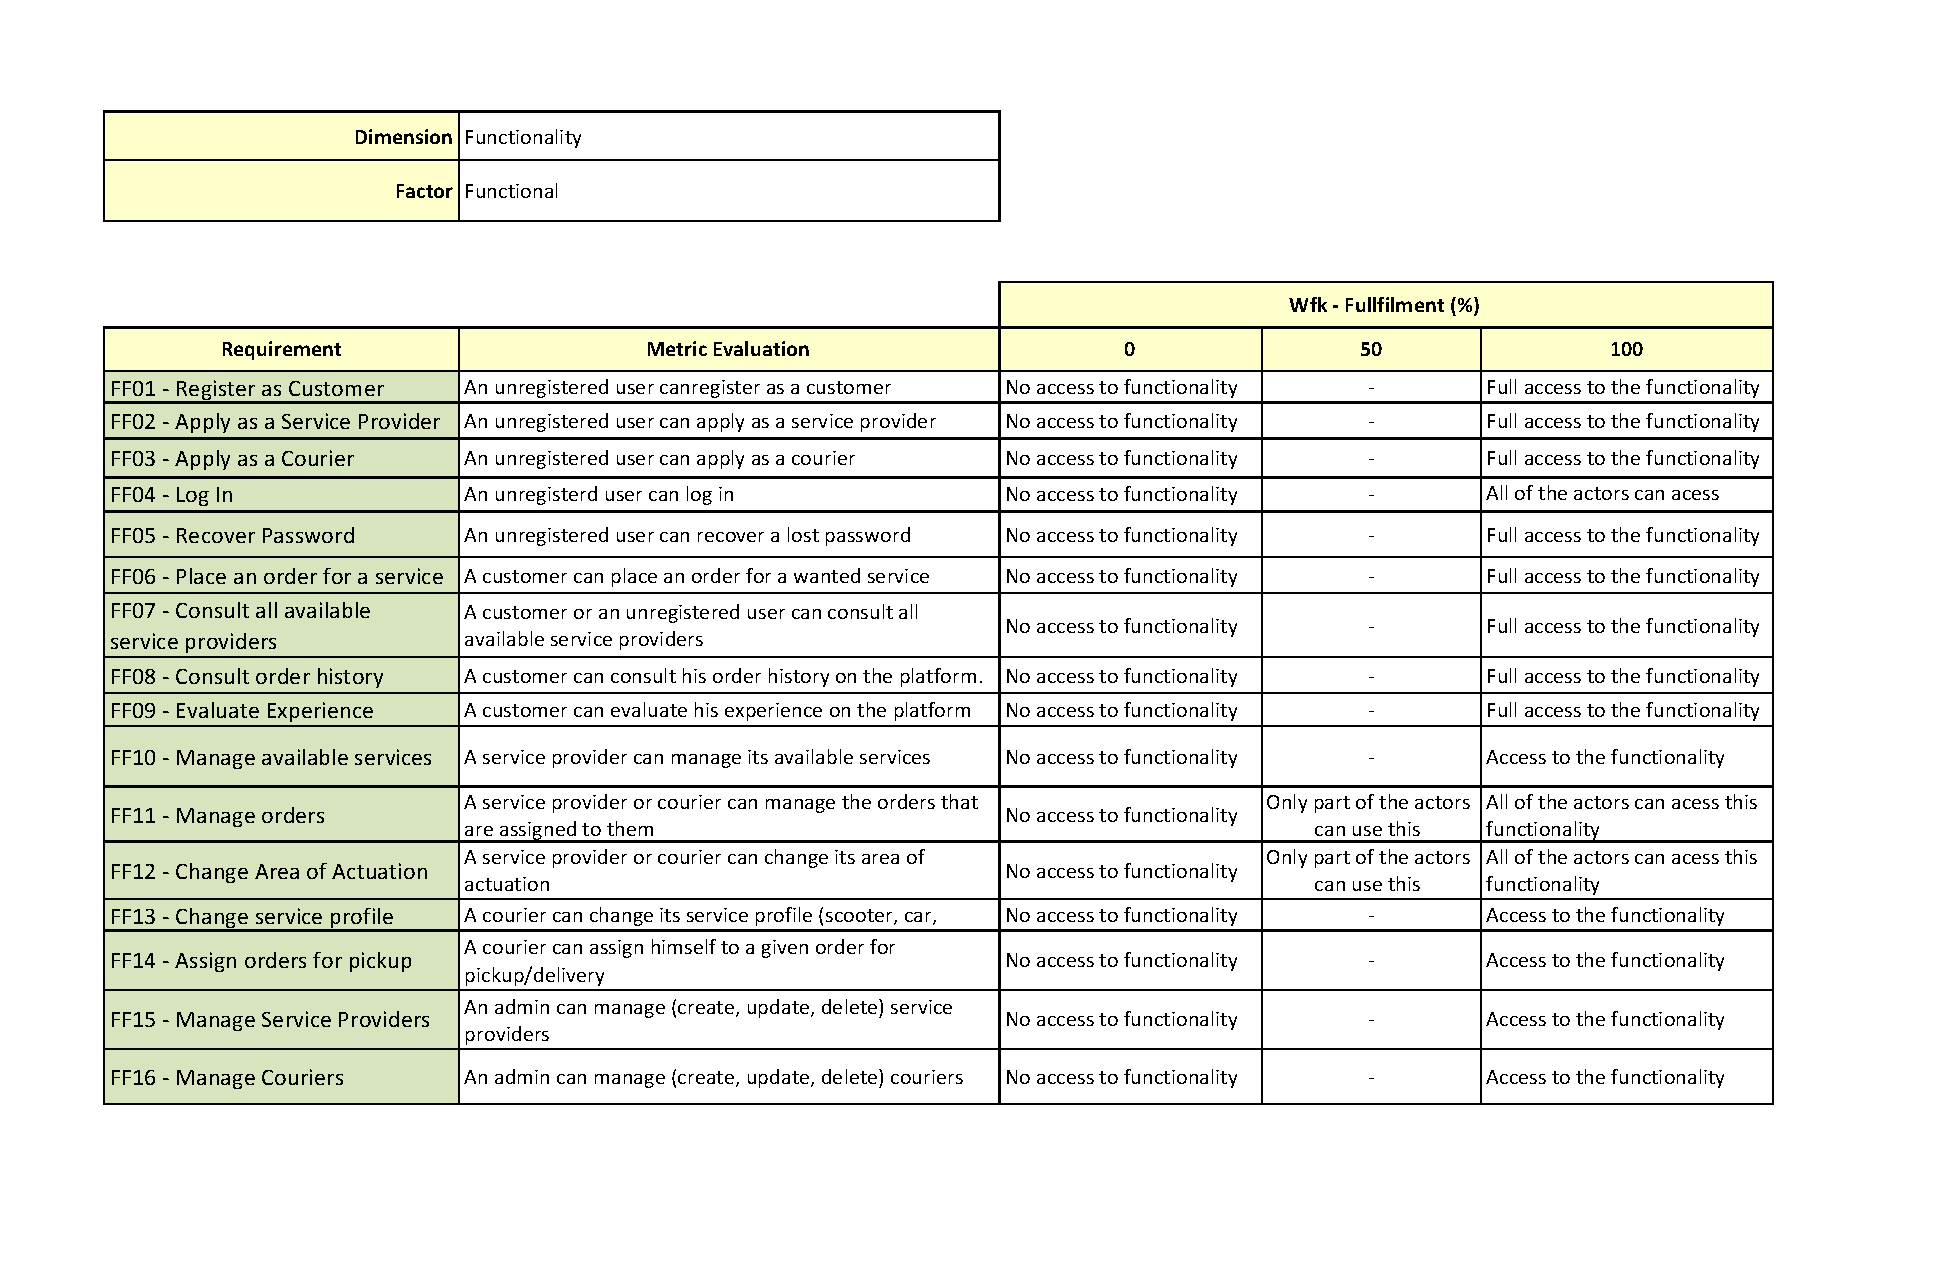
\includegraphics[page=1, angle=90,origin=c, width=0.9\textwidth ]{appendices/QEF/Functionality.pdf}

\pagebreak

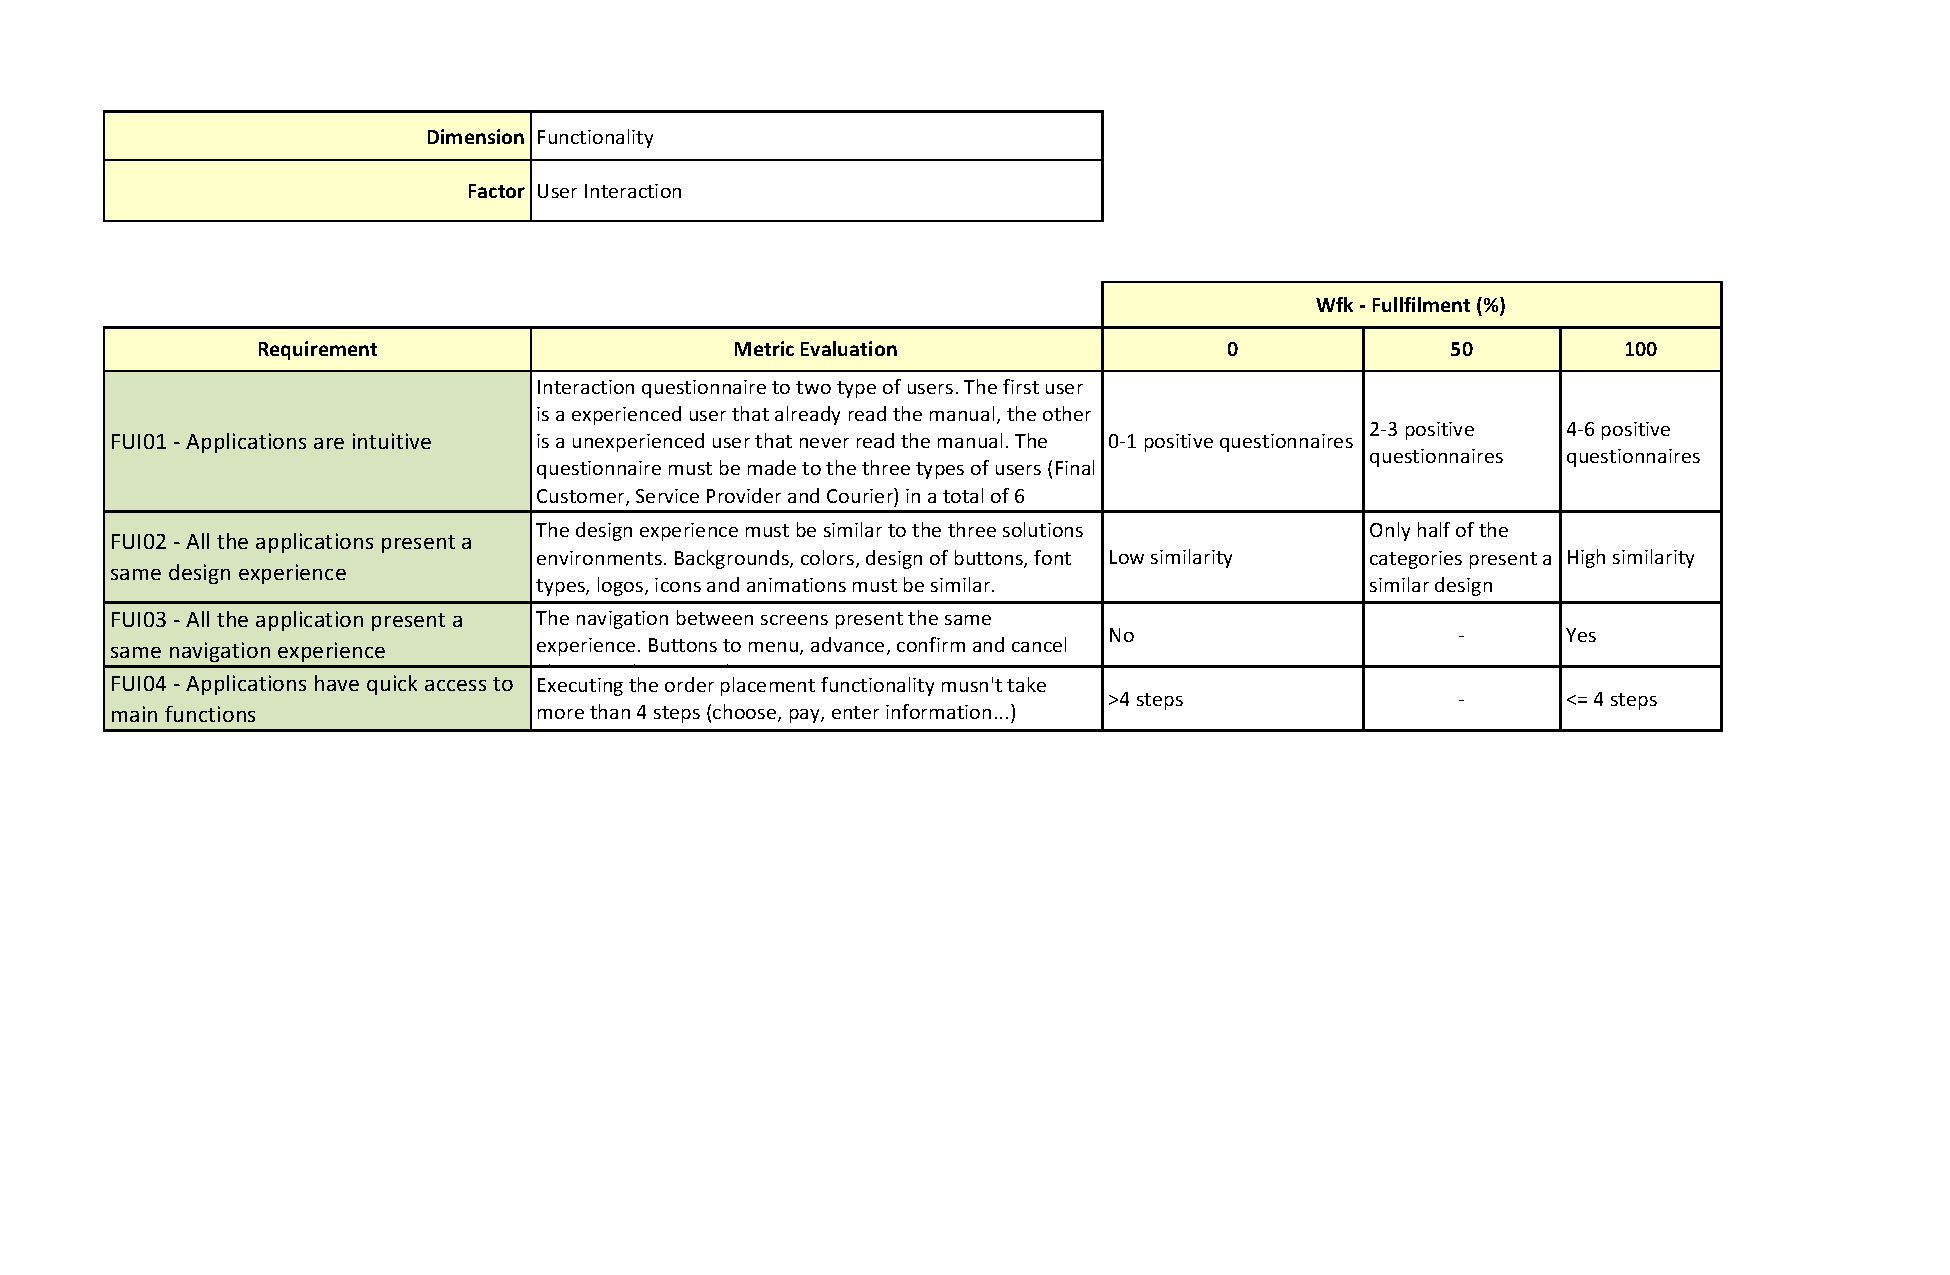
\includegraphics[page=1, angle=90,origin=c, width=\textwidth ]{appendices/QEF/UserInteraction.pdf}

\pagebreak

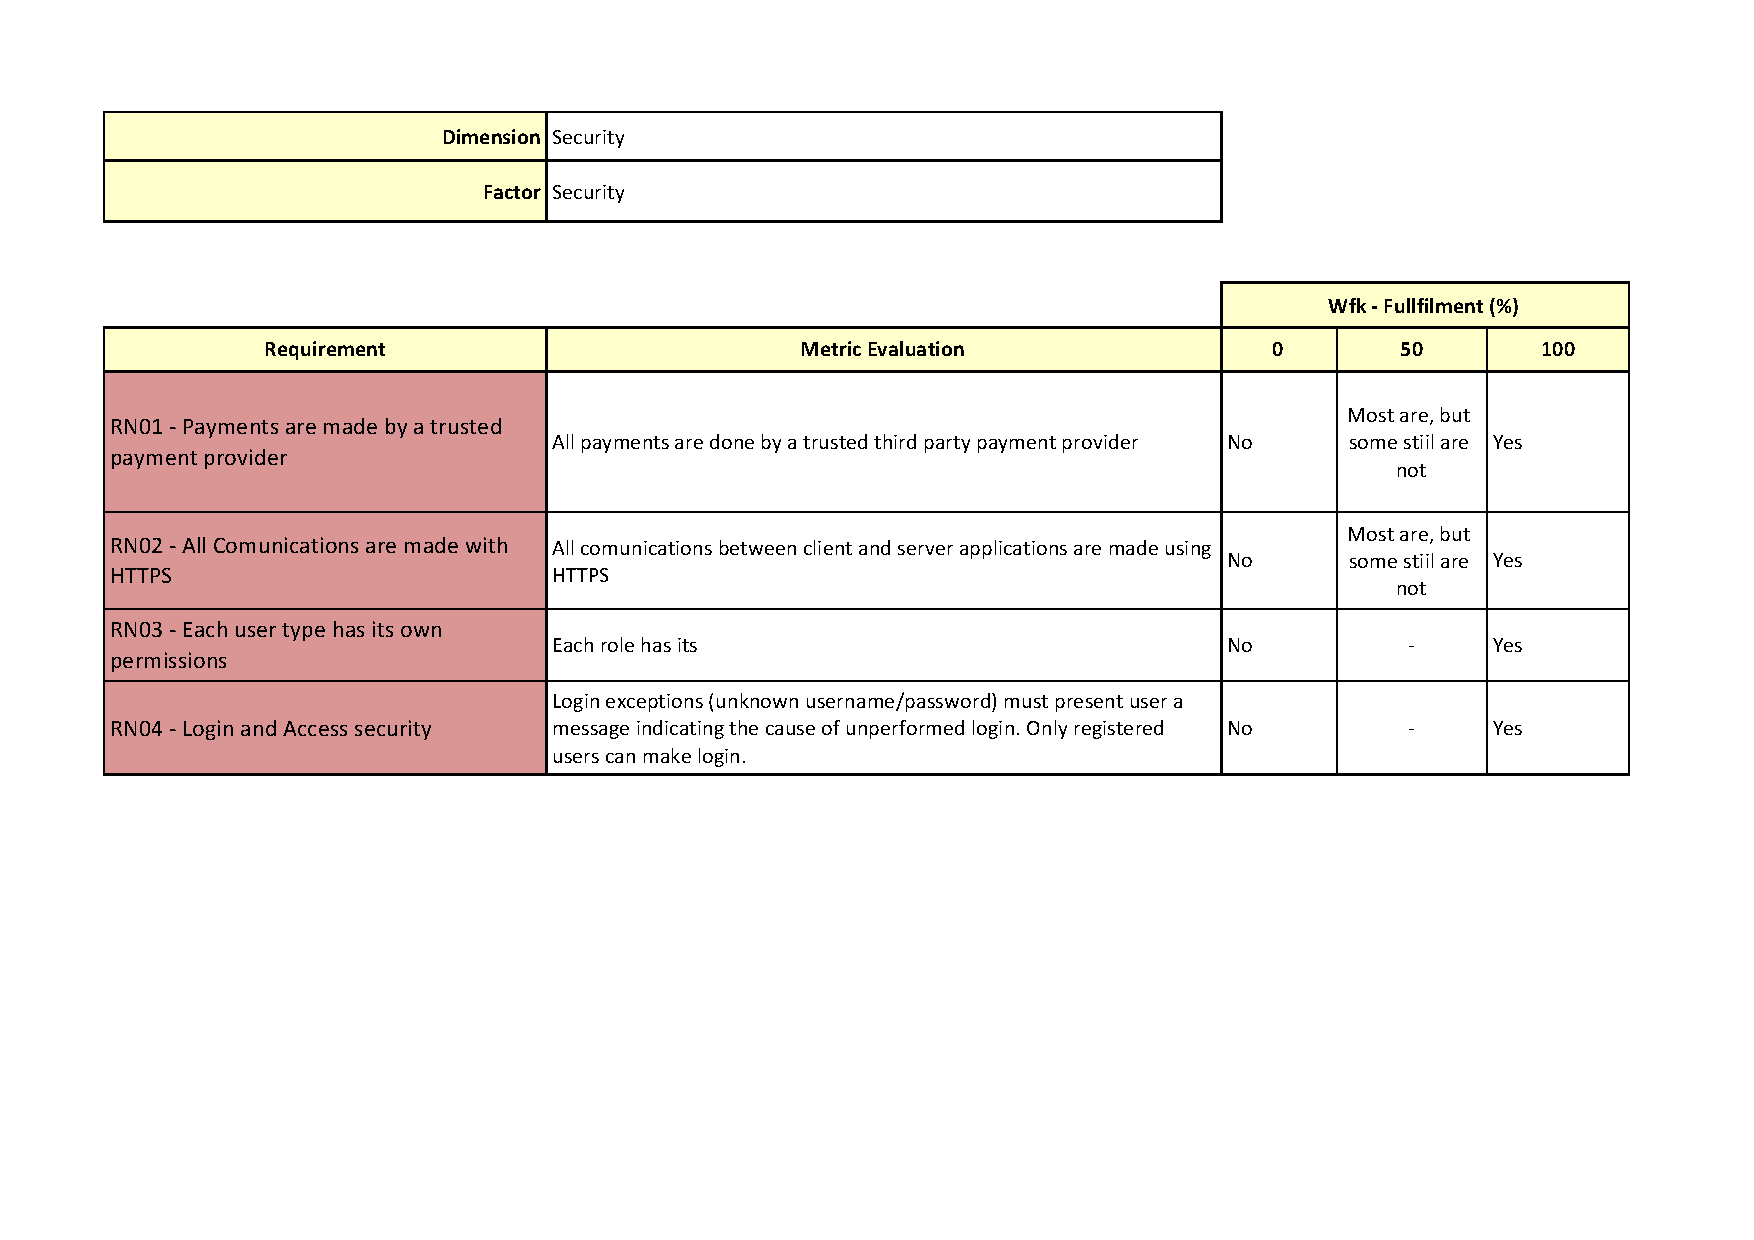
\includegraphics[page=1, angle=90,origin=c, width=\textwidth ]{appendices/QEF/Security.pdf}

\pagebreak

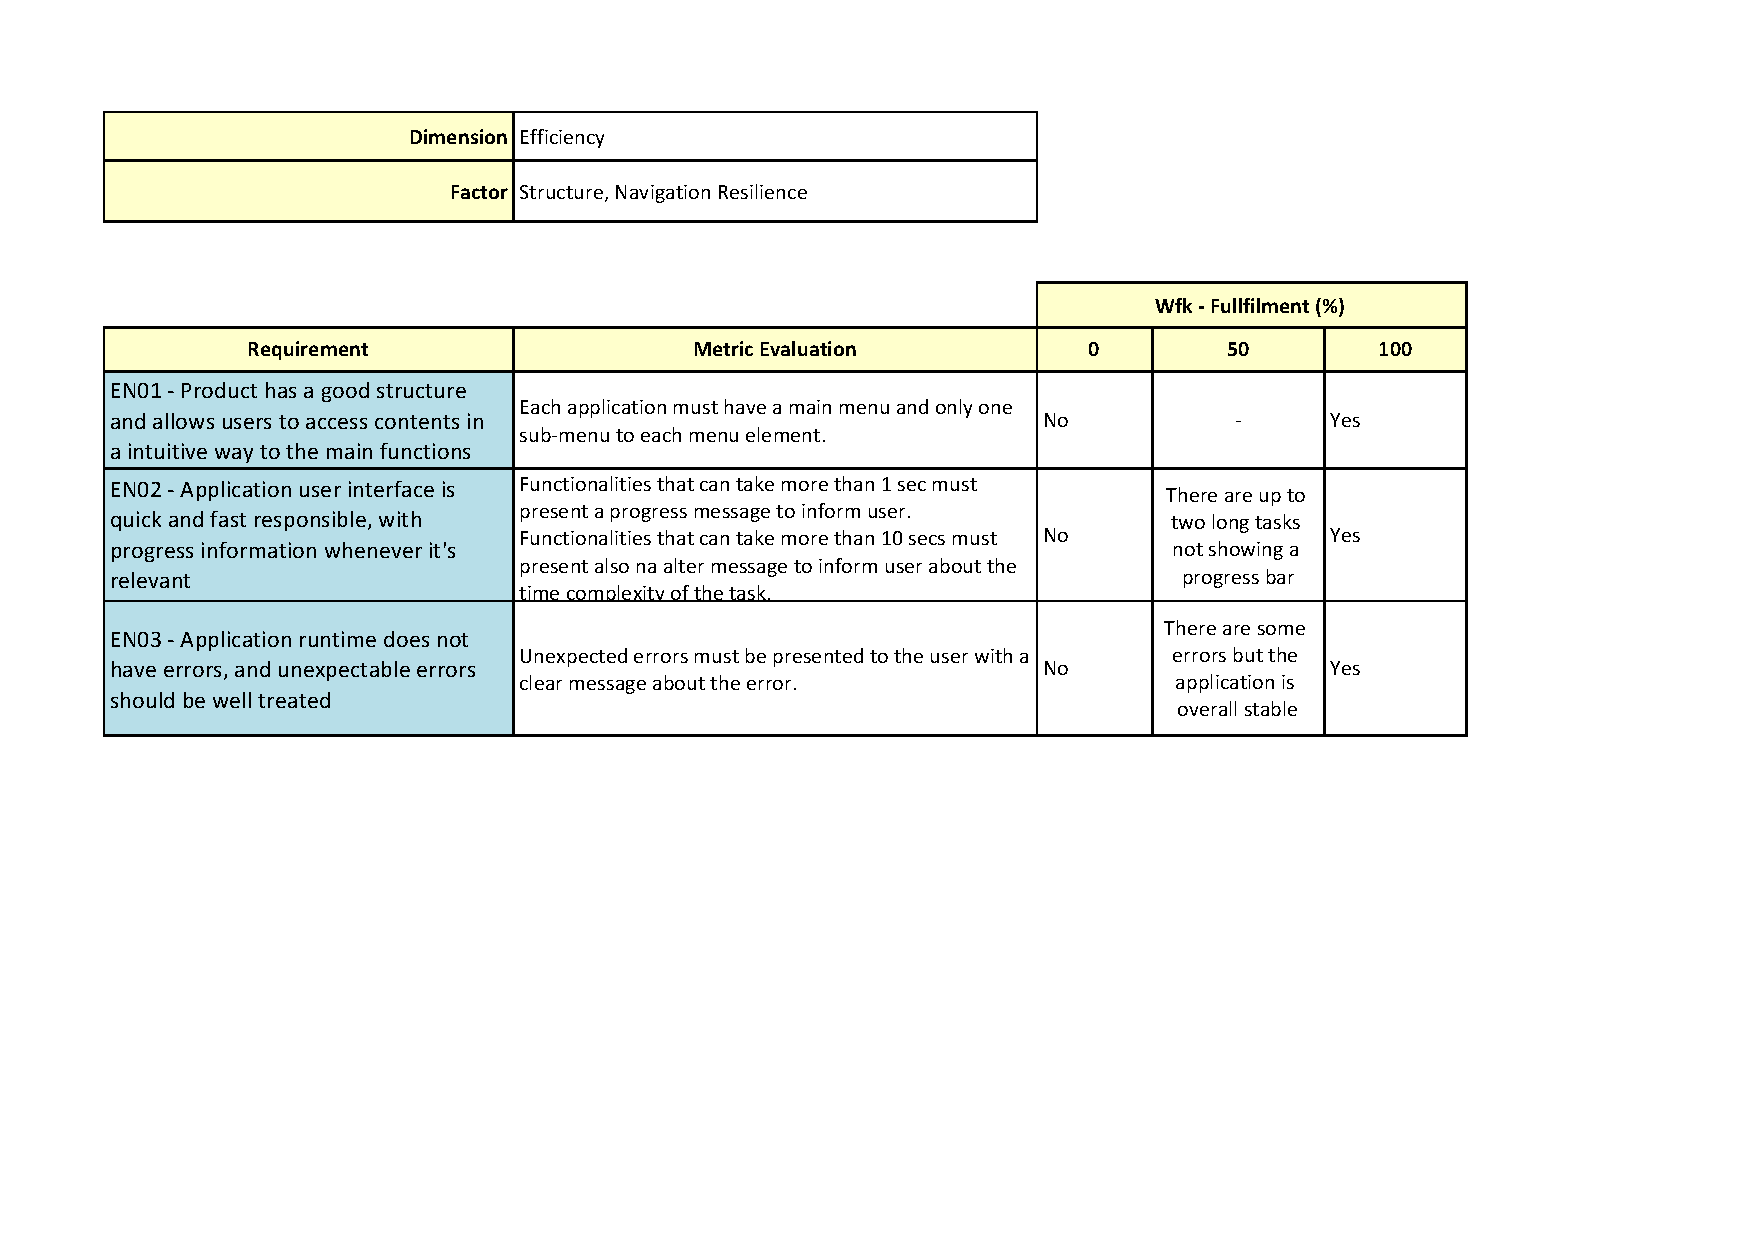
\includegraphics[page=1, angle=90,origin=c, width=\textwidth ]{appendices/QEF/Efficiency.pdf}

\pagebreak

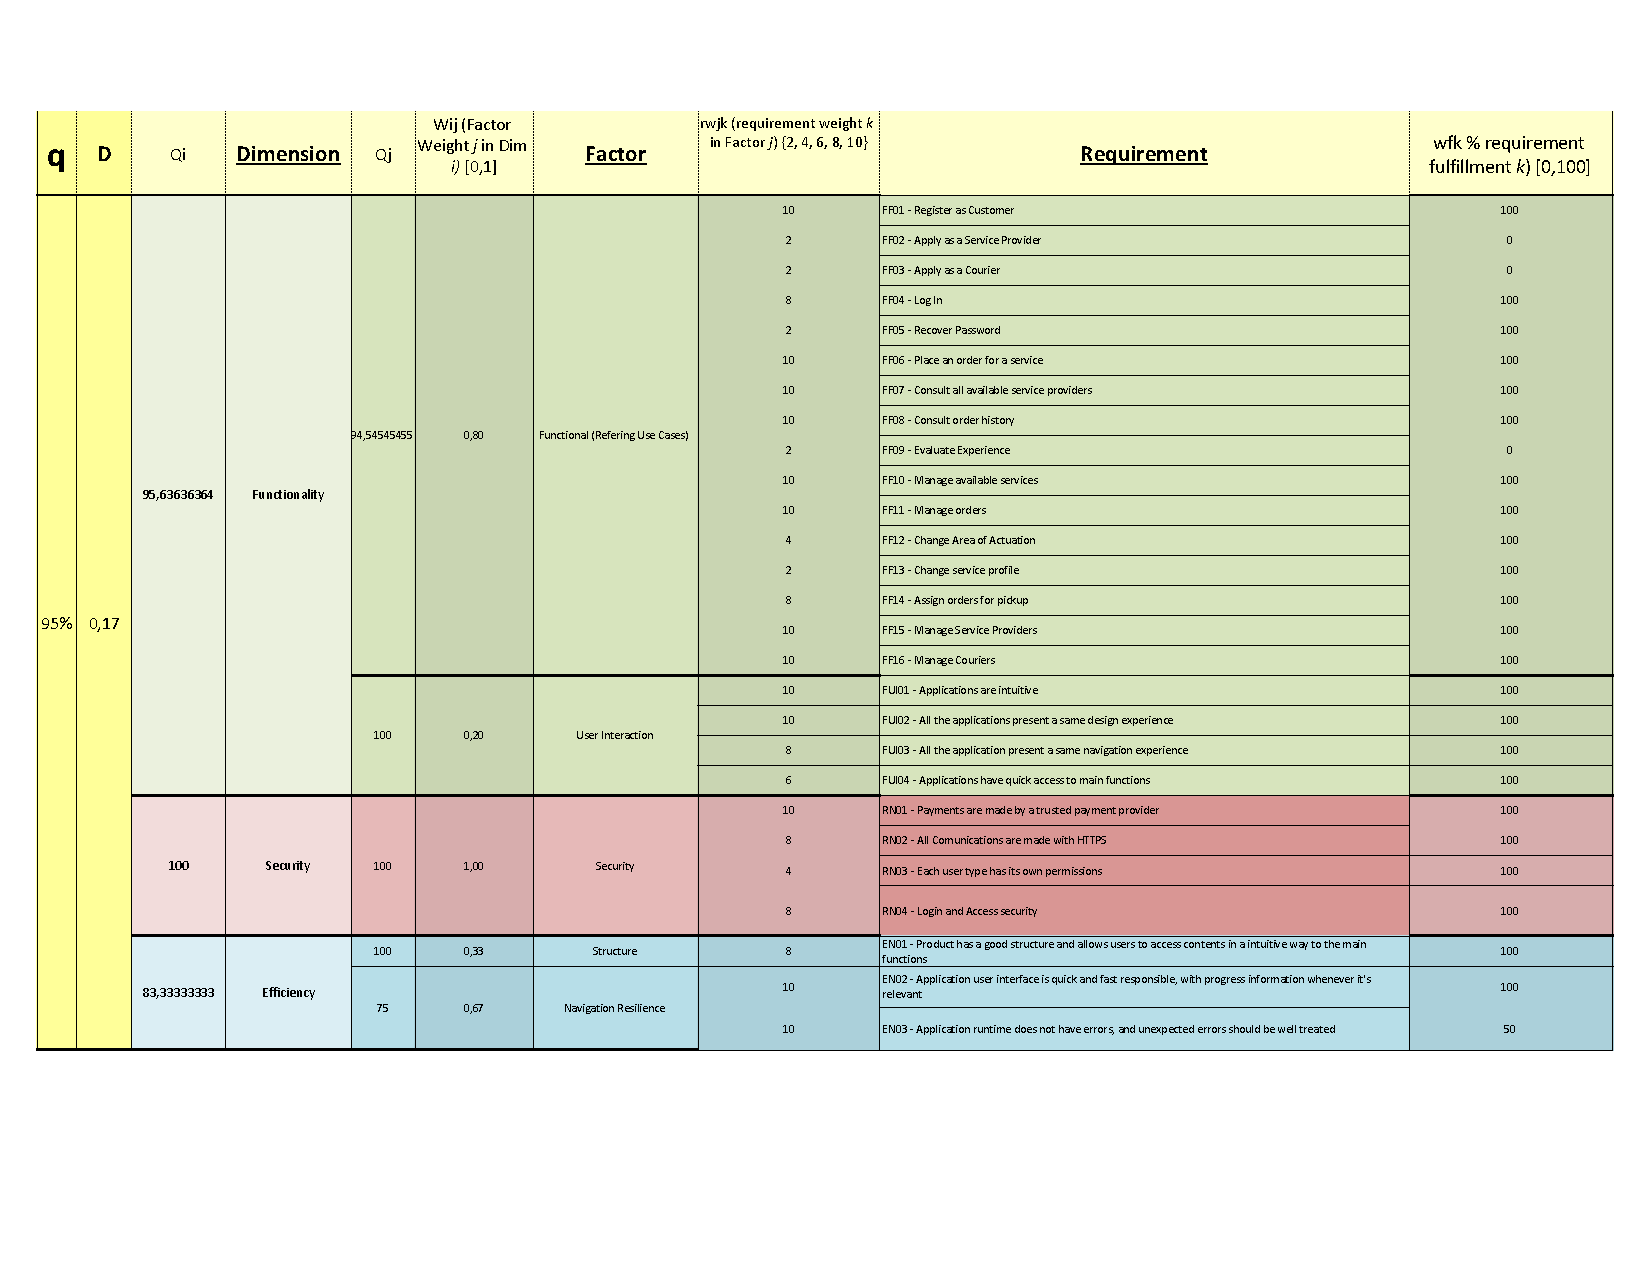
\includegraphics[page=1, angle=90,origin=c, width=1.3\textwidth ]{appendices/QEF/QEF.pdf}

\chapter{Business Model Canvas} % Main appendix title

\label{AppendixC} 

 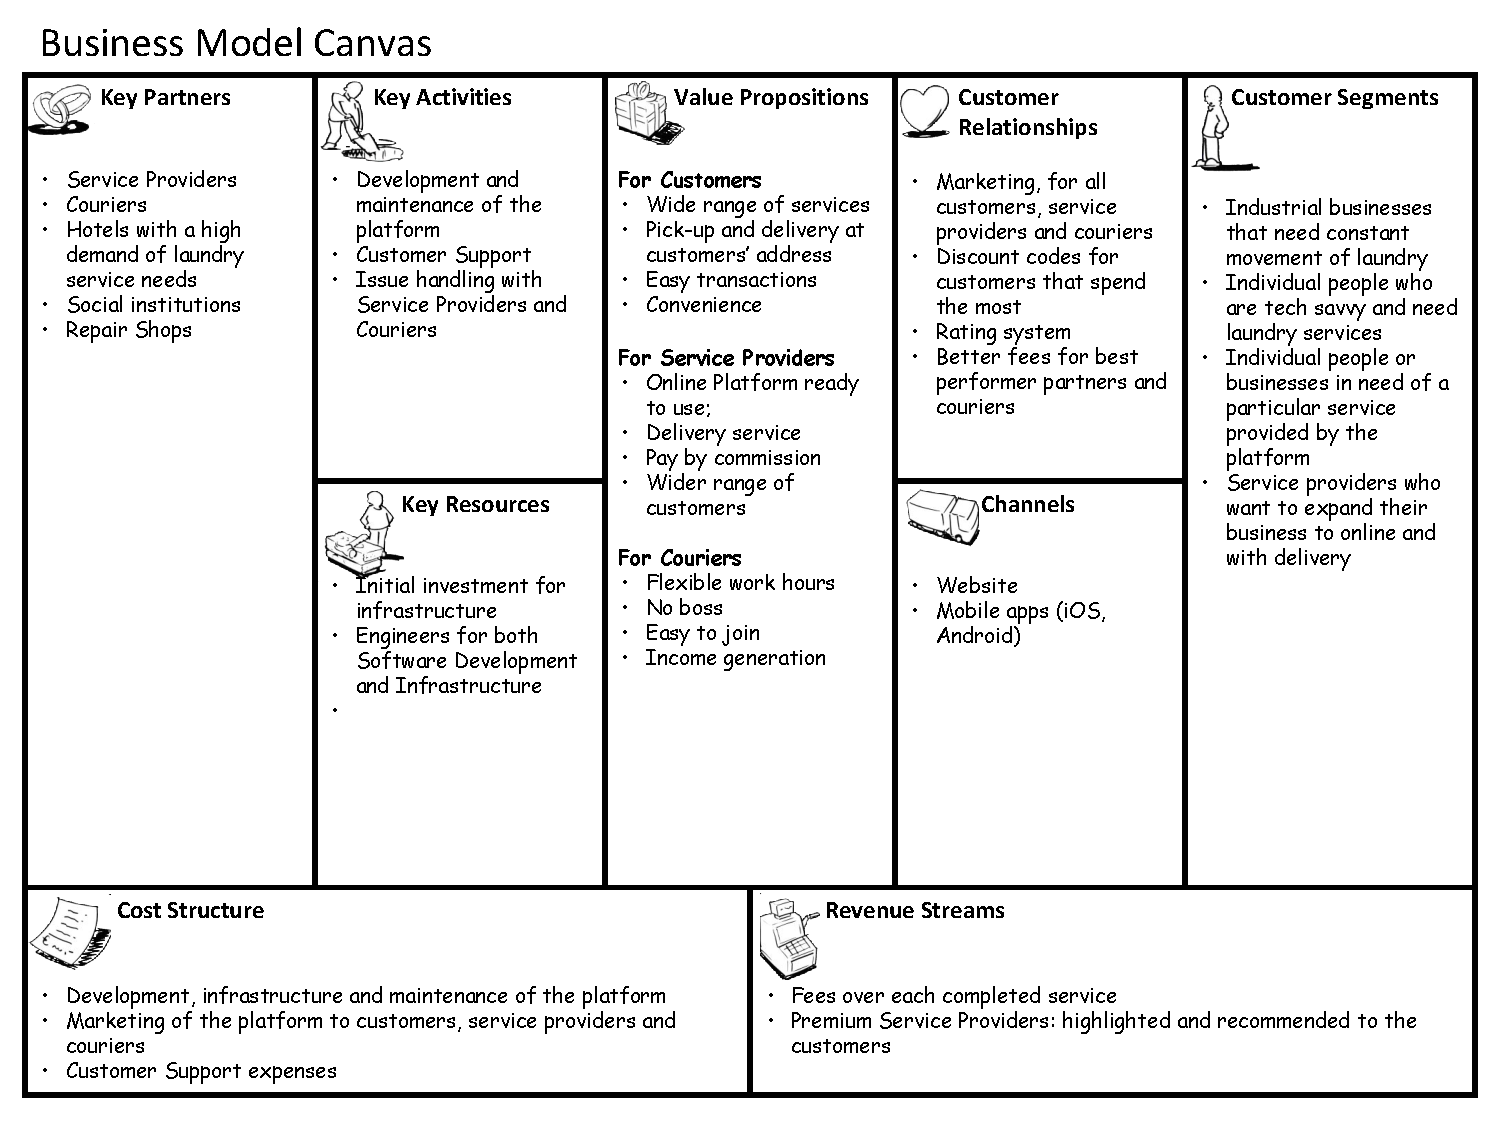
\includegraphics[page=1, angle=90,origin=c, width=0.9\textwidth ]{appendices/files/Canvas.pdf}


\chapter{Customer Perspective Inquiry} % Main appendix title

\label{AppendixD} 

 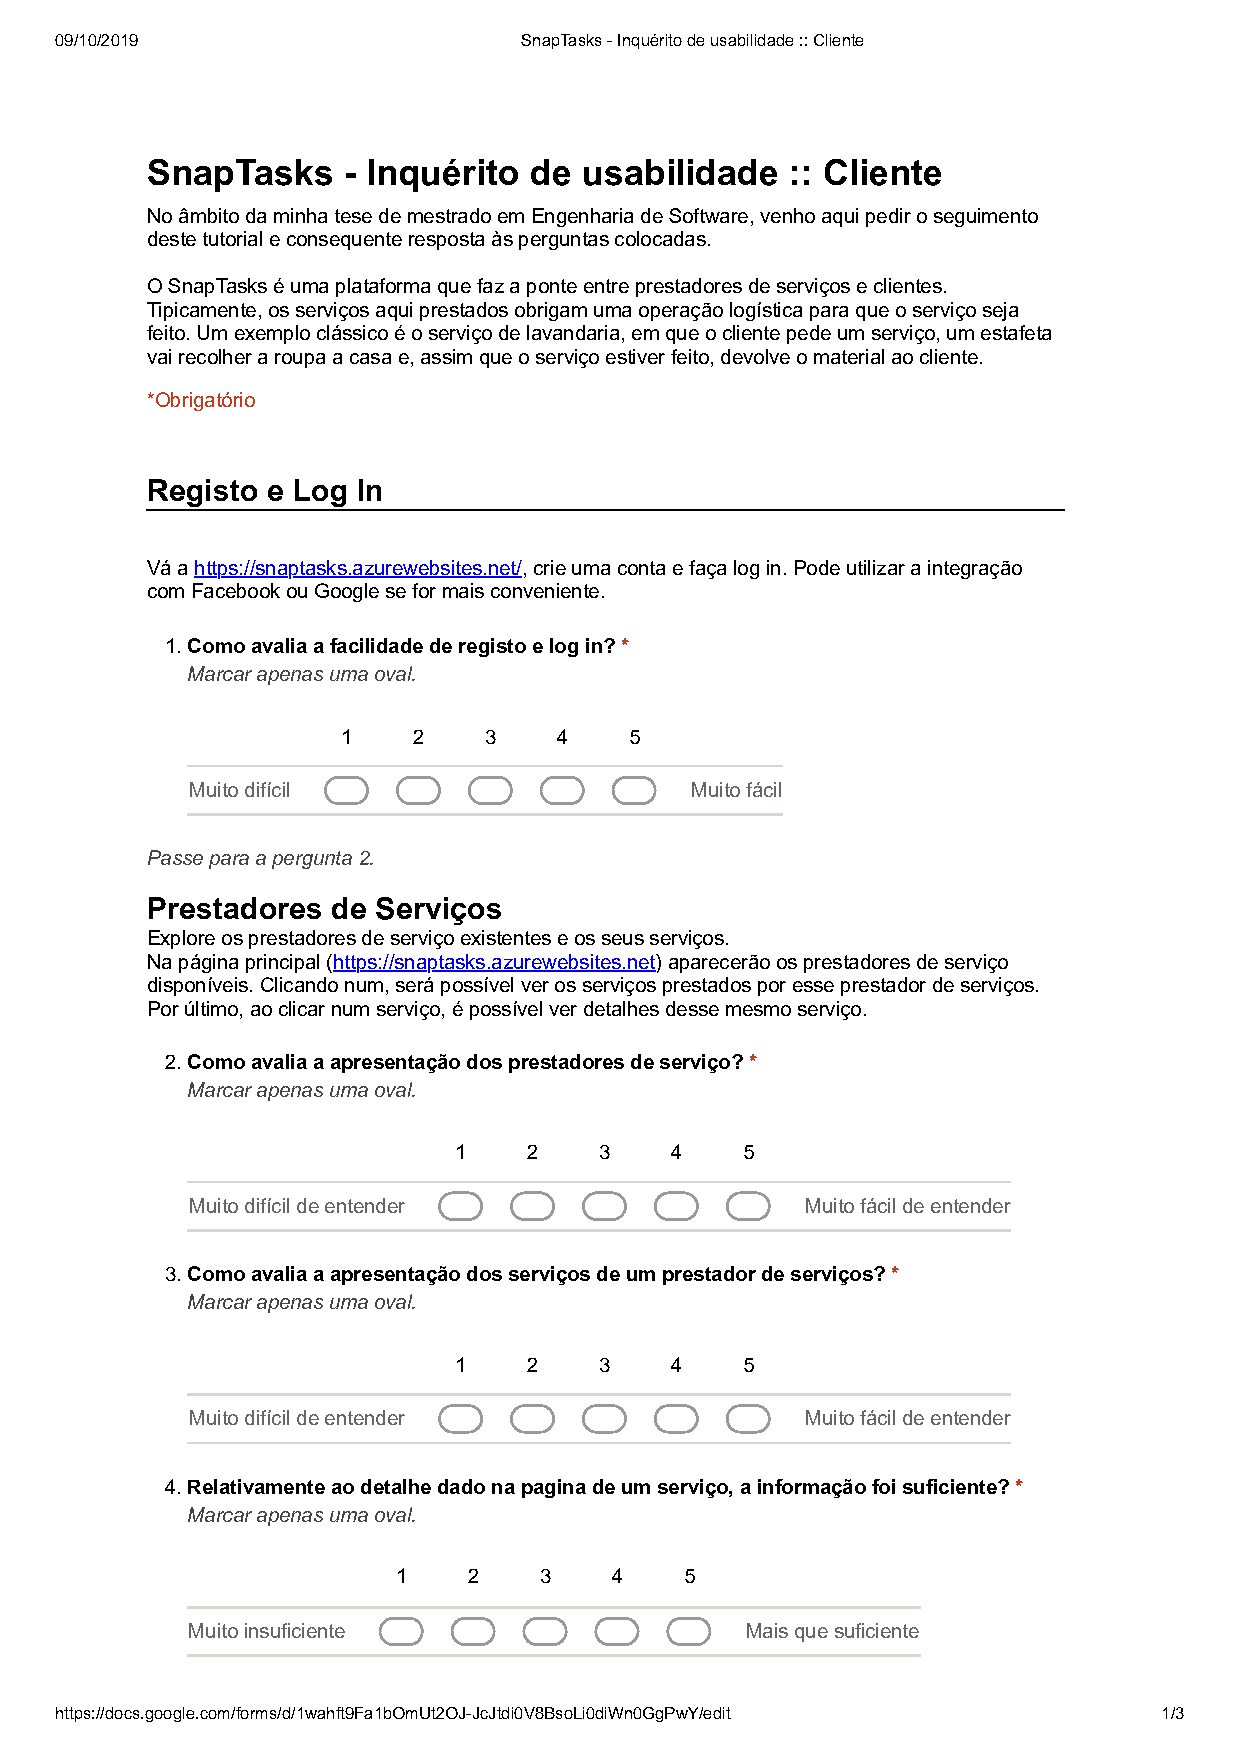
\includegraphics[page=1,origin=c, width=0.9\textwidth ]{appendices/files/inquiry-customer.pdf}

\pagebreak

\includegraphics[page=2,origin=c, width=\textwidth ]{appendices/files/inquiry-customer.pdf}
\pagebreak

\includegraphics[page=3,origin=c, width=\textwidth ]{appendices/files/inquiry-customer.pdf}


\chapter{Service Provider Perspective Inquiry} % Main appendix title

\label{AppendixE} 

 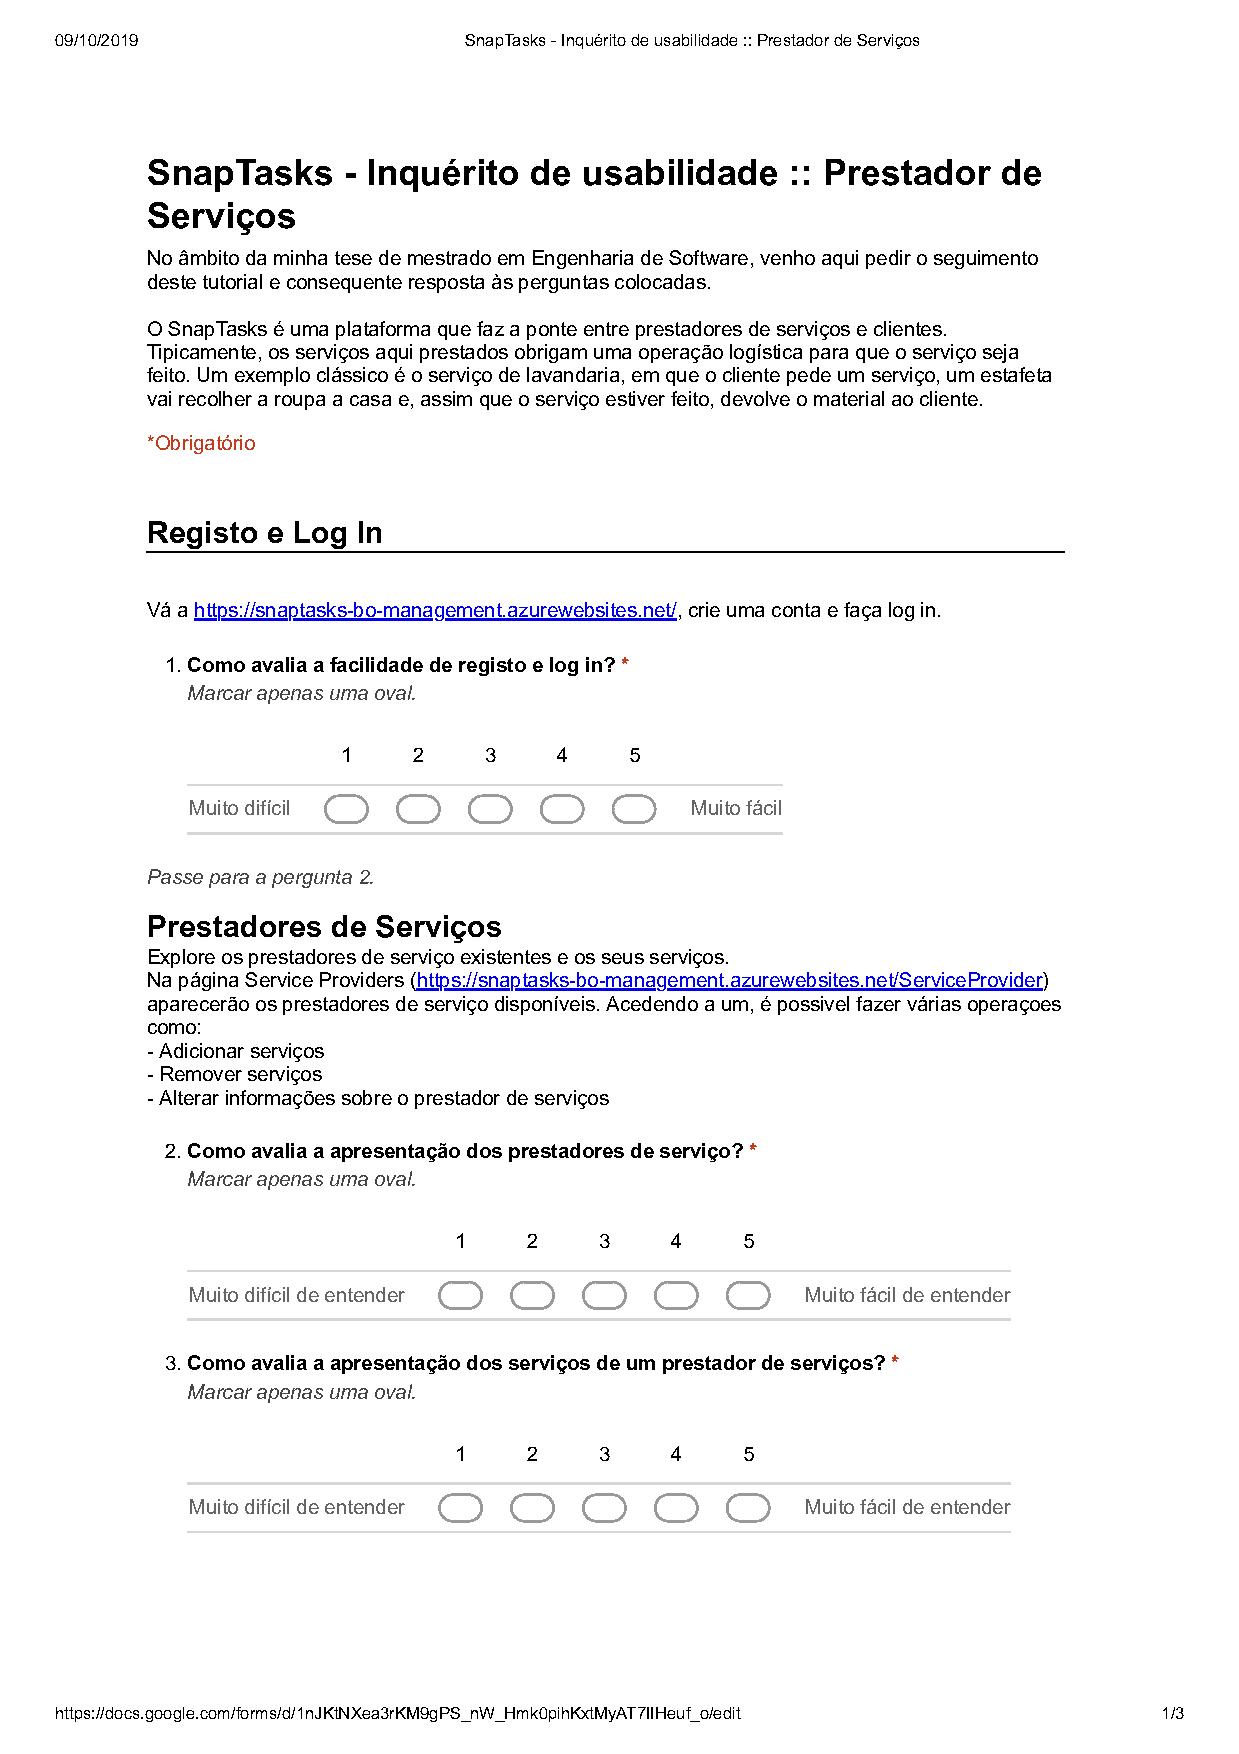
\includegraphics[page=1,origin=c, width=0.9\textwidth ]{appendices/files/inquiry-serviceprovider.pdf}

\pagebreak

\includegraphics[page=2,origin=c, width=\textwidth ]{appendices/files/inquiry-serviceprovider.pdf}

\pagebreak

\includegraphics[page=3,origin=c, width=\textwidth ]{appendices/files/inquiry-serviceprovider.pdf}
\chapter{Customer Perspective Inquiry - Answers} % Main appendix title

\label{AppendixF} 

 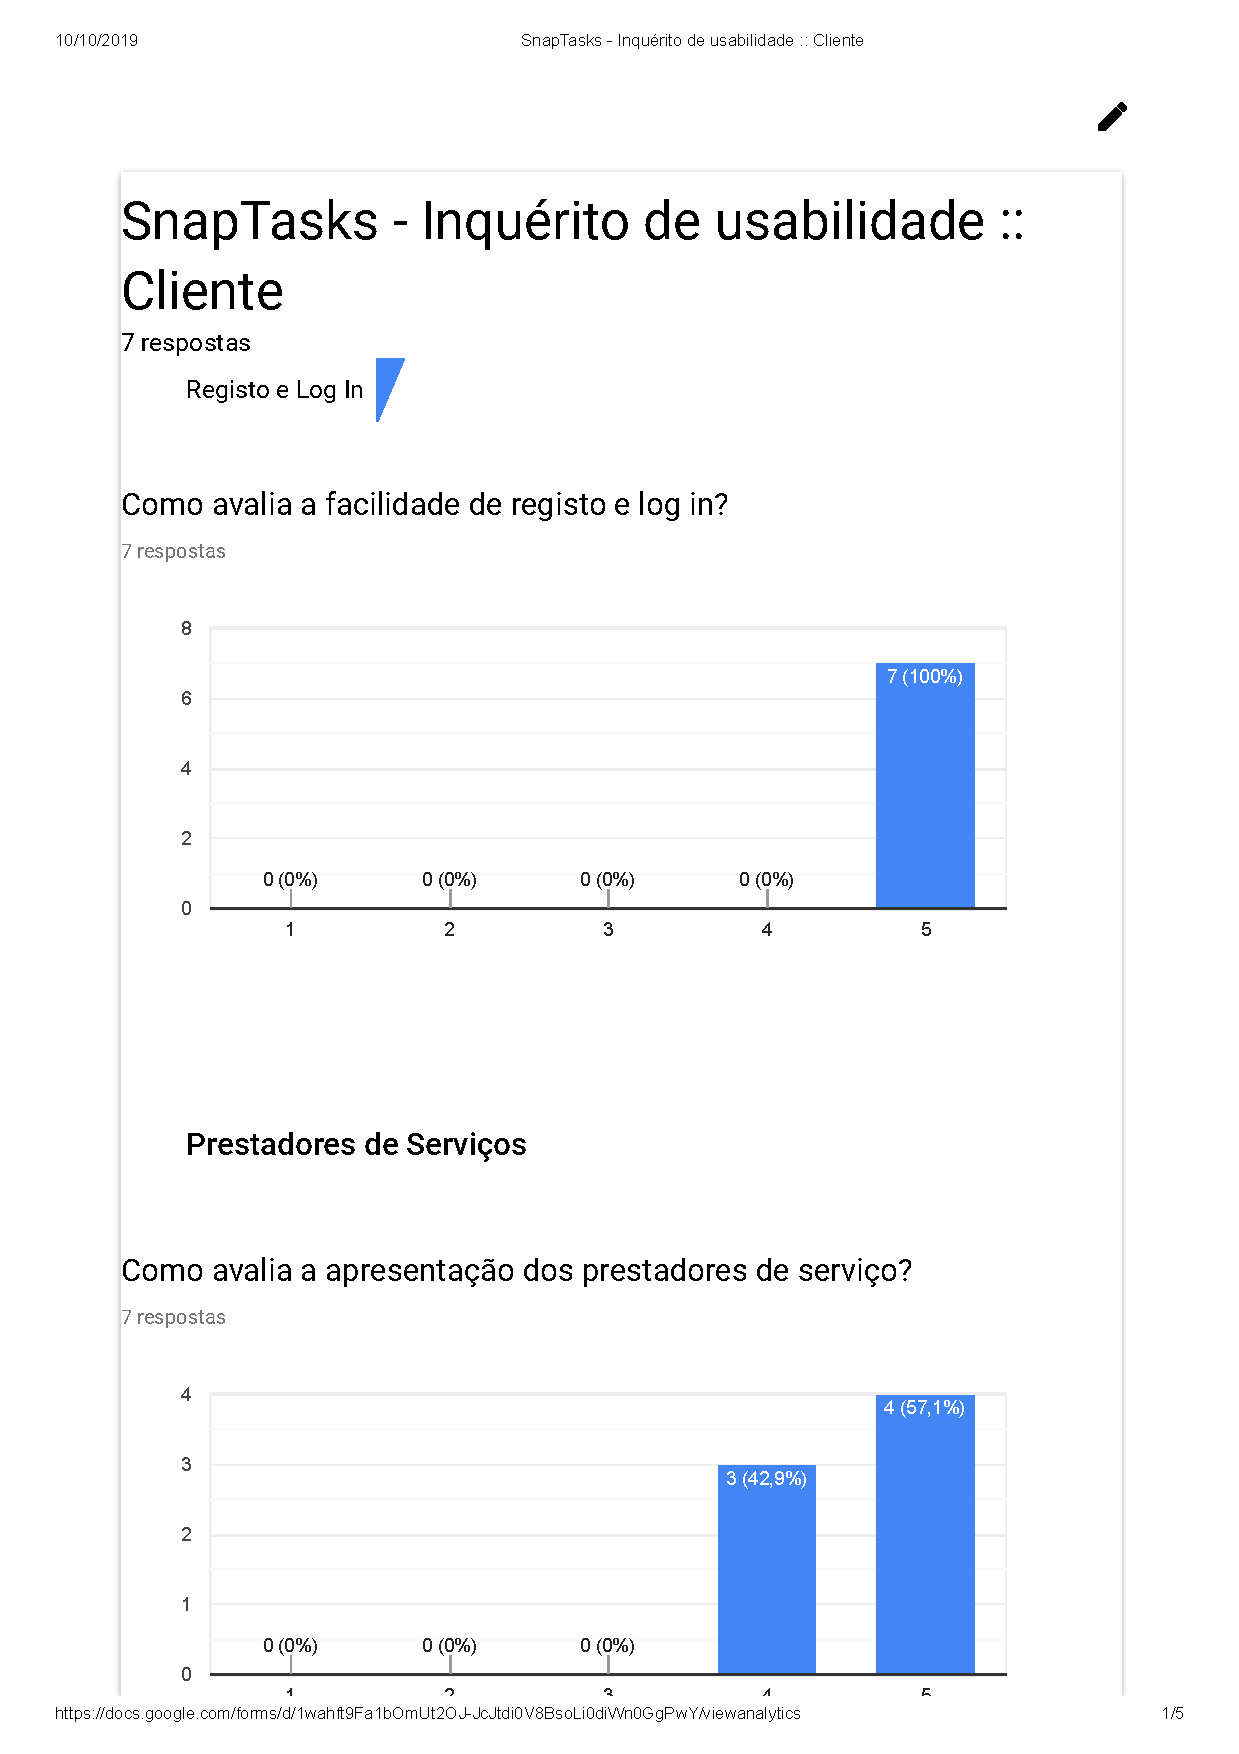
\includegraphics[page=1,origin=c, width=0.9\textwidth ]{appendices/files/InquiryCustomerAnswers.pdf}

\pagebreak

\includegraphics[page=2,origin=c, width=\textwidth ]{appendices/files/InquiryCustomerAnswers.pdf}

\pagebreak

\includegraphics[page=3,origin=c, width=\textwidth ]{appendices/files/InquiryCustomerAnswers.pdf}

\pagebreak

\includegraphics[page=4,origin=c, width=\textwidth ]{appendices/files/InquiryCustomerAnswers.pdf}

\pagebreak

\includegraphics[page=5,origin=c, width=\textwidth ]{appendices/files/InquiryCustomerAnswers.pdf}
\chapter{Service Provider Perspective Inquiry - Answers} % Main appendix title

\label{AppendixG} 

 \includegraphics[page=1,origin=c, width=0.9\textwidth ]{appendices/files/InquiryServiceProvidersAnswers.pdf}

\pagebreak

\includegraphics[page=2,origin=c, width=\textwidth ]{appendices/files/InquiryServiceProvidersAnswers.pdf}

\pagebreak

\includegraphics[page=3,origin=c, width=\textwidth ]{appendices/files/InquiryServiceProvidersAnswers.pdf}

\pagebreak

\includegraphics[page=4,origin=c, width=\textwidth ]{appendices/files/InquiryServiceProvidersAnswers.pdf}

\pagebreak

\includegraphics[page=5,origin=c, width=\textwidth ]{appendices/files/InquiryServiceProvidersAnswers.pdf}

\pagebreak

\includegraphics[page=6,origin=c, width=\textwidth ]{appendices/files/InquiryServiceProvidersAnswers.pdf}

%----------------------------------------------------------------------------------------

\end{document}
